%\documentclass[printer]{gOMS2e}
%\documentclass[runningheads,a4paper,singlecolumn]{llncs}
\documentclass[printer]{article}

%\documentclass[11pt]{article}

%\doi{10.1080/1055.6788.2012.xxxxxx}
%\issn{1029-4937}
%\issnp{1055-6788}
%\jvol{00} \jnum{00} \jyear{2012} \jmonth{November}

%\markboth{Taylor \& Francis and I.T. Consultant}{Optimization Methods and Software}

%\usepackage{hyperref}
%\usepackage{ulem}
\usepackage{amssymb}
\setcounter{tocdepth}{3}
\usepackage{graphicx}
\usepackage{sidecap}

\usepackage{url}
%\pagestyle{myheadings}       % it must be
%\usepackage[dvips]{graphicx}
\usepackage{graphicx}
\usepackage{times}
%\usepackage{subfigure}
%\usepackage{epsfig}
\usepackage{setspace}
\usepackage{latexsym}
\usepackage{algorithm}
\usepackage[noend]{algpseudocode}
\usepackage{wrapfig}
\usepackage{sidecap}
\usepackage{booktabs}

\usepackage{caption}
\usepackage{subcaption}

\renewcommand{\baselinestretch}{1.05}             % Improves readability

%\def\qed{\vrule height .9ex width .8ex depth -.1ex}

%\setlength{\subfigcapskip}{0pt}

\def\floatpagefraction{0.99} 
\def\clq{\mbox{\sc Clique}}
\def\mclq{\mbox{\sc MaxClique}}
\def\clqh{\mbox{\sc CliqueHeu}}
\def\mclqh{\mbox{\sc MaxCliqueHeu}}
\def\beforesubfigures{-0.55cm}
\def\beforesectiontitle{-0.4cm}
\def\aftersectiontitle{-0.2cm}
\def\afterfigure{-0.2cm}
%\def\scale{7.25cm}
\def\scaleN{3.9cm}
\def\scale{5cm}
\def\rowspace{-1pt}
\def\figlabelsize{\scriptsize}
%\def\algospacing{0.85}
\def\algospacing{1.0}

\newcommand{\algorithmroutine}[1]{-- \textit{#1}}

\begin{document}

\title{Fast Algorithms for the Maximum Clique Problem on Massive Sparse Graphs}

\author{Bharath Pattabiraman$^{\rm \ast \ddag}$, Md. Mostofa Ali Patwary$^{\rm \ast \ddag}$, \\ Assefaw H. Gebremedhin$^{\rm \dag}$, Wei-keng Liao$^{\rm \ast}$, and Alok Choudhary
%\thanks{Email: $^{\rm \ast}$\{bpa342,mpatwary,wkliao,choudhar\}@eecs.northwestern.edu, $^{\rm \dag}$agebreme@purdue.edu\vspace{6pt}}
\thanks{$^{\rm \ddag}$ Corresponding authors: \{bpa342,mpatwary\}@eecs.northwestern.edu \vspace{6pt}}
\\
$^{\rm \ast}${\em{Northwestern University, Evanston, IL 60208}} \\
$^{\rm \dag}${\em Purdue University, West Lafayette, IN 47907}
\\
%\vspace{10pt}
$^{\rm \ddag}$ Authors contributed equally \\ 
%$^{\rm \ddag}$ Corresponding authors: \{bpa342,mpatwary\}@eecs.northwestern.edu\\ 
}
%\received{November 2012} }


%\author{Bharath Pattabiraman%\inst{1}
%\andMd. Mostofa Ali Patwary%\inst{1}
%\and \\Assefaw H. Gebremedhin%\inst{2}
%\and Wei-keng Liao%\inst{1}
%\and Alok Choudhary%\inst{1}
%$\\$^{\rm \ddag}$ Authors contributed equally \\ 
%}

%\institute{
%Northwestern University, Evanston, IL.\\ \email{\{bpa342,mpatwary,wkliao,choudhar\}@eecs.northwestern.edu}
%\and
%Purdue University, West Lafayette, IN.\\ \email{agebreme@purdue.edu}
%}

%\authorrunning{Bharath Pattabiraman et al.} % abbreviated author list (for running head)
%\tocauthor{Authors' Instructions}

%\toctitle{Lecture Notes in Computer Science}

\maketitle

\date{}
%\vspace{-4pt}

\begin{abstract}
%\vspace{\afterfigure}
%\vspace{\afterfigure}

%%% AHG: testing git pull
The maximum clique problem is a well known NP-Hard problem with
applications in data mining, network analysis, information retrieval and many other
areas related to the World Wide Web.
There exist several algorithms for the problem with acceptable runtimes for
certain classes of graphs, but many of them are infeasible for massive graphs. 
We present a new exact algorithm that employs novel pruning techniques and 
is able to quickly find maximum cliques in large sparse graphs. 
Extensive experiments on different kinds of synthetic and 
real-world graphs show that our new algorithm can be orders of magnitude 
faster than existing algorithms.
We also present a heuristic that runs orders of magnitude faster than 
the exact algorithm while providing optimal or near-optimal solutions.


%\keywords{maximum clique problem, branch-and-bound algorithms,  pruning, sparse graphs.}
\end{abstract}

%\vspace{-24pt}

\section{Introduction}
\label{sec:intro}
%\vspace{-6pt}

A clique in an undirected graph is a subset of vertices in which every two vertices
are adjacent to each other. The {\em maximum} clique problem seeks to find 
a clique of the largest possible size in a given graph.

The maximum clique problem, and the related {\em maximal} clique and 
clique {\em enumeration} problems, find applications in a wide variety of domains,
many intimately related to the World Wide Web. 
A few examples include:  
information retrieval \cite{Augustson:1970:AGT:321607.321608}, 
community detection in networks \cite{Fortunato_2010,cite-key,5586496}, 
spatial data mining \cite{wang2009order},
data mining in bioinformatics \cite{19566964},
disease classification based on symptom correlation \cite{Bonner:1964:CT:1662386.1662389}, 
pattern recognition \cite{1211348},
analysis of financial networks \cite{RePEc:eee:csdana:v:48:y:2005:i:2:p:431-443},
computer vision \cite{Horaud:1989:SCT:68871.68875}, and
coding theory \cite{brouwer}.
More examples of application areas can be found in 
\cite{Gutin2004,citeulike:4058448}.

To get a sense for how clique computation arises in the aforementioned contexts, 
consider a generic data mining or information retrieval problem. A typical objective
here is to retrieve data that are considered similar based on some metric. 
Constructing a graph in which vertices correspond to data items and 
edges connect similar items, a clique in the graph would then give a cluster of similar data. 

The maximum clique problem is NP-Hard \cite{Garey:1979:CIG:578533}.
Most exact algorithms for solving it employ some form of {\it branch-and-bound} approach. 
While branching systematically searches for all candidate solutions, bounding (also known as {\em pruning}) discards fruitless candidates based on a previously computed bound. 
The algorithm of Carraghan and Pardalos \cite{pardalos} is an early example of 
a simple and  effective branch-and-bound algorithm for the maximum clique problem.
%are \cite{Bomze99themaximum,pardalos}. 
More recently,  \"{O}sterg\.{a}rd \cite{ostergard} introduced 
an improved algorithm and demonstrated its relative advantages via computational experiments. 
Tomita and Seki \cite{citeulike:7905505}, and later, Konc and Jane\v{z}i\v{c} \cite{konc2007improved}
use upper bounds computed using vertex coloring to enhance the branch-and-bound approach. 
%Sewell (1998) presented a maximum clique algorithm designed for dense graphs.
Other examples of branch-and-bound algorithms for the clique problem include 
the works of Bomze et al~\cite{Bomze99themaximum}, Segundo et al~\cite{SanSegundo}
and Babel and Tinhofer~\cite{babel1990branch}.
Prosser~\cite{prosser2012} in a recent work compares various exact algorithms 
for the maximum clique problem. %An attractive feature of the algorithms of \cite{pardalos} and \cite{ostergard} is their simplicity in terms of ease of implementation. However, their runtimes could  be infeasible for very large graphs.

%only for graphs with up to a few thousand vertices and a corresponding number of edges. 
%Furthermore, both algorithms as well as 
%the algorithms from  \cite{citeulike:7905505} and \cite{konc2007improved}
%are inherently sequential and not naturally parallelizable. 
%The ease with which an algorithm can be parallelized is important 
%for handling large-scale graphs in emerging applications, where graphs with 
%millions (or more) vertices are quite common \cite{kumar:extracting}.

In this paper, we present a new exact branch-and-bound
algorithm for the maximum clique problem that employs 
several new pruning strategies in addition to those used in \cite{pardalos},
\cite{ostergard},  \cite{citeulike:7905505} and \cite{konc2007improved},
making it suitable for massive graphs.
%We also present a heuristic that is based on similar pruning techniques as the exact algorithm but runs much faster---the heuristic follows just one of the ``paths" in the search space, and as a result its complexity is nearly linear-time in the size of the graph, in contrast to the exact algorithm whose worst-case complexity is exponential. 
We run our algorithms on a large variety of test graphs and compare its performance with the
algorithm of Carraghan and Pardalos \cite{pardalos}, the algorithm of \"{O}sterg\.{a}rd \cite{ostergard} and the algorithm of Konc and Jane\v{z}i\v{c} \cite{konc2007improved}. 
We find our new exact algorithm to be up to orders of magnitude faster on large,
sparse graphs and of comparable runtime on denser graphs.
We also present a hew heuristic, which runs several orders of magnitude faster than the exact algorithm while providing solutions that are optimal or near-optimal for most cases.
The algorithms are presented in Section~\ref{sec:algorithms} and the experimental evaluations and comparisons are presented in Section~\ref{sec:experiments}. 

Both the exact algorithm and the heuristic are well-suited for parallelization.
We discuss a simple shared-memory parallelization and present performance 
results showing its promise in Section~\ref{sec:parallelization}. 
We also include (in Section~\ref{sec:applications})
a small illustration on how the algorithms can be used as parts of a method
for detecting overlapping communities in social networks.
We have made our implementations publicly available\footnote{\url{http://cucis.ece.northwestern.edu/projects/MAXCLIQUE/}}.
%The algorithms are discussed in detail in Section~\ref{sec:algorithms}.

%In Section~\ref{sec:experiments} we present an extensive experimental analysis comparing the performance of our algorithms with the algorithm of Carraghan and Pardalos \cite{pardalos}, the algorithm of \"{O}sterg\.{a}rd \cite{ostergard} and the algorithm of Konc and Jane\v{z}i\v{c} \cite{konc2007improved}.
%The workings of the latter three algorithms is reviewed in Section~\ref{sec:relatedwork}.

%Our testbed includes large-scale real-world graphs drawn from various application domains, large-scale synthetic graphs representing various structures, and DIMACS benchmark graphs.

% \cite{dimacs}, 
%the University of Florida collection, 
%\cite{Davis97theuniversity}, 
% \cite{Chakrabarti:2006:GML:1132952.1132954},
%\vspace{-10pt}



%\section{The Carraghan-Pardalos and  \"{O}sterg\.{a}rd Algorithms}
\section{Related Previous Algorithms}
\label{sec:relatedwork}
%\vspace{-6pt}

Given a simple undirected graph $G$, the maximum clique can clearly be obtained by enumerating 
{\em all} of the cliques present in it and picking the largest of them.
Carraghan and Pardalos \cite{pardalos} introduced a simple-to-implement
algorithm that avoids enumerating all cliques and instead
works with a significantly reduced partial enumeration.
The reduction in enumeration is achieved via 
a {\em pruning} strategy which reduces the search space tremendously.
The algorithm works by
performing at each step $i$, a {\em depth first search} from vertex $v_i$, 
where the goal is to find the largest clique containing the vertex $v_i$.
At each {\em depth} of the search, the algorithm compares the number of remaining
vertices that could potentially constitute a clique containing vertex $v_i$
against the size of the largest clique encountered thus far.
If that number is found to be smaller, the algorithm backtracks (search is pruned).

\"{O}sterg\.{a}rd \cite{ostergard} devised an algorithm that incorporated an additional 
pruning strategy to the one by Carraghan and Pardalos.
The opportunity for the new pruning strategy is created by {\em reversing} the order in which the search is done by
the Carraghan-Pardalos algorithm. This allows for an additional pruning with the help of
some auxiliary bookkeeping. 
Experimental results in \cite{ostergard} showed that the \"{O}sterg\.{a}rd
algorithm is faster than the Carraghan-Pardalos algorithm on random and 
DIMACS benchmark graphs \cite{dimacs}.
However, the new pruning strategy used in this algorithm is intimately tied to the order in which vertices are processed, introducing an inherent sequentiality into the algorithm.
% which renders it unsuitable for easy parallelization.

A number of existing branch-and-bound algorithms for maximum clique
also use a vertex-coloring of the graph to obtain an upper bound on the maximum clique. 
%A {\em vertex-coloring} of a graph is an assignment of colors to vertices such that  a pair of adjacent vertices receive different colors. Clearly, the number of colors used gives  an upper bound on the maximum clique of the graph, which can be used to reduce the search space. 
A popular and recent method based on this idea is 
the MCQ algorithm of Tomita and Seiku \cite{citeulike:7905505}. 
More recently, Konc and Jane\v{z}i\v{c} \cite{konc2007improved} presented 
an improved version of MCQ, known as MaxCliqueDyn (with the variants MCQD and MCQD+CS), 
that involves the use of tighter, computationally more expensive upper bounds 
applied on a fraction of the search space.

%They present two variations - 1) MCQ with improved 
%approximate coloring algorithm ColorSort (MCQ+CS) and 2) MCQ with improved coloring and dynamic sorting 
%of vertices (MCQD+CS)). The authors observe the latter to outperform MCQ on random and DIMACS benchmark graphs.

%\vspace{-12pt}


\section{The New Algorithms}
\label{sec:algorithms}
%\vspace{-6pt}
We describe in this section new algorithms that overcome the shortcomings mentioned earlier; 
the new algorithms use additional pruning strategies, maintain simplicity, and 
avoid a sequential computational order.
We begin by first introducing the following notations.
%Let $G = (V,E)$ denote a simple undirected graph, and let $n = \left|V\right|$ and $m = \left|E\right|$. 
We identify the $n$ vertices of the input graph $G=(V,E)$ as $\{v_1, v_2, \ldots, v_n\}$.  
The set of vertices adjacent to a vertex $v_i$, the set of its neighbors, is denoted by $N(v_i)$.
And the degree of the vertex $v_i$, the cardinality of $N(v_i)$, is 
denoted by $d(v_i)$.  

%\vspace{-10pt}
\subsection{The Exact Algorithm}
\label{subsec:exact}
%\vspace{-4pt}

Recall that the maximum clique in a graph can be found by computing the largest clique containing each vertex and picking the largest among these. 
A key element of our exact algorithm is that during the search for the largest clique containing a given vertex, vertices that cannot form cliques larger than the current maximum 
clique are {\em pruned}, in a hierarchical fashion. 
The method is outlined in detail in Algorithm \ref{alg:mClq}. 
Throughout, the variable $max$ stores the size of the maximum clique found 
thus far. Initially it is set to be equal to the lower bound $lb$ provided as an input parameter.
It gives the maximum clique size when the algorithm terminates.

\begin{figure}
%\vspace{14pt}
\hrule
\vspace{6pt}
\begin{spacing}{\algospacing}
{
{\small
\captionof{algorithm}{{\protect\small Algorithm for finding the maximum clique of a given graph.
{\it Input}: Graph $G = \left (V, E\right )$, lower bound on clique $lb$ (default, 0). {\it Output}: Size of maximum clique.}}\label{alg:mClq}
\vspace{-5pt}
\hrule
\vspace{6pt}

\noindent\begin{minipage}{.5\textwidth}
\vspace{-12pt}
\begin{algorithmic}[1]
\Procedure {MaxClique}{$G=\left (V,E\right )$, $lb$}
\State $max \leftarrow lb$
\For{$i:1$ to $n$}
%\If{$degree(v_i) < maxClq$} 
%\State continue \Comment{{\small Pruning 1}}
%\EndIf
\If{$d(v_i) \ge max$} \Comment{{\footnotesize Pruning 1}} \label{pr1}
\State $U \leftarrow \emptyset$
\For{each $v_j \in N(v_i)$}
\If{$j > i$} \Comment{{\footnotesize Pruning 2}} \label{prOld}
\If{$d(v_j) \ge max$} \Comment{{\footnotesize Pruning 3}} \label{pr2}
\State $U \leftarrow U \cup \{v_j\}$ 
\EndIf
\EndIf
\EndFor

\State \textsc{Clique}$(G, U, 1)$ \label{subCall}
\EndIf

\EndFor
\EndProcedure
\end{algorithmic}
\end{minipage}%
\begin{minipage}{.5\textwidth}
\captionof*{algorithm}{{\em Subroutine}}
\vspace{-6pt}
\begin{algorithmic}[1]
\Procedure {Clique}{$G=\left (V,E\right )$, $U$, $size$}

\If{$U = \emptyset$}
\If{$size > max$} 
\State $max \leftarrow size$ \label{critical}
\EndIf
\State {\bf return}
\EndIf

\While{$\left|U\right| > 0$}
\If{$size + \left|{U}\right| \le max$} \Comment{{\footnotesize Pruning 4}} \label{pr3}
\State {\bf return} 
\EndIf

\State Select any vertex $u$ from $U$ 
%of maximum degree in $G$

\State $U \leftarrow U \setminus \{u\} $
\State $N'(u):= \{w | w \in N(u) \wedge d(w) \ge max\}$  \Comment{{\footnotesize Pruning 5}} \label{pr4}
\State \textsc{Clique}$( G, U \cap N'(u), size + 1)$
\EndWhile

\EndProcedure
\end{algorithmic}
\end{minipage}
}
}
\end{spacing}
\vspace{8pt}
\hrule
%\vspace{10pt}
\end{figure}

To obtain the largest clique containing a vertex $v_i$, 
it is sufficient to consider only the neighbors of $v_i$. 
The main routine {\sc MaxClique} thus generates  for each 
vertex $v_i \in V$ a set $U \subseteq N(v_i)$ 
(neighbors of $v_i$ that survive pruning) and calls the subroutine \clq\ on $U$.  
The subroutine \clq\ goes through every relevant clique containing $v_i$ 
in a recursive fashion and returns the largest.
%, and a more elaborate explanation can be found there. 
We use $size$ to maintain the size of the clique found at any point through the recursion.
Since we start with a clique of just one vertex, the value of $size$ is set to one initially, 
when \clq\ is called (Line \ref{subCall}, {\sc MaxClique}).




%\begin{figure}[!ht]
%\centering
%\hrule
%\vspace{5pt}
%\caption{{\protect\small Algorithm for finding the maximum clique of a given graph.
%{\it Input}: Graph $G = \left (V, E\right )$, lower bound on clique $lb$ (default, 0). 
%{\it Output}: Size of maximum clique.}}
%\vspace{-4pt}
%\hrule
%\vspace{8pt}
%\begin{subfigure}{.48\textwidth}
%\centering
%\begin{algorithmic}
%\Procedure {MaxClique}{$G=\left (V,E\right )$, $lb$}
%\State $max \leftarrow lb$
%\For{$i:1$ to $n$}
%%\If{$degree(v_i) < maxClq$} 
%%\State continue \Comment{{\small Pruning 1}}
%%\EndIf
%\If{$d(v_i) \ge max$} \Comment{{\footnotesize Pruning 1}} \label{pr1}
%\State $U \leftarrow \emptyset$
%\For{each $v_j \in N(v_i)$}
%\If{$j > i$} \Comment{{\footnotesize Pruning 2}} \label{prOld}
%\If{$d(v_j) \ge max$} \Comment{{\footnotesize Pruning 3}} \label{pr2}
%\State $U \leftarrow U \cup \{v_j\}$ 
%\EndIf
%\EndIf
%\EndFor
%
%\State \textsc{Clique}$(G, U, 1)$ \label{subCall}
%\EndIf
%
%\EndFor
%\EndProcedure
%\end{algorithmic}
%%\caption{Test Algorithm No.1}\label{alg:alg-1}
%\end{subfigure}
%\hfill
%\begin{subfigure}{.48\textwidth}
%\centering
%\begin{algorithmic}
%\If{$d(v_j) \ge max$} \Comment{{\footnotesize Pruning 3}}
%\State $U \leftarrow U \cup \{v_j\}$ 
%\EndIf
%\end{algorithmic}
%%\caption{Test Algorithm No.2}\label{alg:alg-2}
%\end{subfigure}
%\vspace{5pt}
%\hrule
%%\caption{Two algorithms side by side}\label{fig:twoalg}
%\end{figure}


%\begin{minipage}{0.6\textwidth}
%\begin{algorithm}[t]
%\begin{spacing}{\algospacing}
%{
%\small
%\caption{{\protect\small Algorithm for finding the maximum clique of a given graph.
%{\it Input}: Graph $G = \left (V, E\right )$, lower bound on clique $lb$ (default, 0). 
%{\it Output}: Size of maximum clique.}}
%%The vertex set $V$ is assumed to be {\em ordered}.
%%\vspace{4pt}
%%\algorithmroutine{Main routine}
%%%\rule{0.65\textwidth}{.1mm}
%%\vspace{4pt}
%
%\label{alg:mClq}
%\begin{algorithmic}[1]
%\Procedure {MaxClique}{$G=\left (V,E\right )$, $lb$}
%\State $max \leftarrow lb$
%\For{$i:1$ to $n$}
%%\If{$degree(v_i) < maxClq$} 
%%\State continue \Comment{{\small Pruning 1}}
%%\EndIf
%\If{$d(v_i) \ge max$} \Comment{{\footnotesize Pruning 1}} \label{pr1}
%\State $U \leftarrow \emptyset$
%\For{each $v_j \in N(v_i)$}
%\If{$j > i$} \Comment{{\footnotesize Pruning 2}} \label{prOld}
%\If{$d(v_j) \ge max$} \Comment{{\footnotesize Pruning 3}} \label{pr2}
%\State $U \leftarrow U \cup \{v_j\}$ 
%\EndIf
%\EndIf
%\EndFor
%
%\State \textsc{Clique}$(G, U, 1)$ \label{subCall}
%\EndIf
%
%\EndFor
%\EndProcedure
%\end{algorithmic}
%}
%\vspace{-4pt}
%\rule{1\textwidth}{.1mm}\\
%
%\algorithmroutine{Subroutine}
%{
%\begin{algorithmic}[1]
%\Procedure {Clique}{$G=\left (V,E\right )$, $U$, $size$}
%
%\If{$U = \emptyset$}
%\If{$size > max$} 
%\State $max \leftarrow size$ \label{critical}
%\EndIf
%\State {\bf return}
%\EndIf
%
%\While{$\left|U\right| > 0$}
%\If{$size + \left|{U}\right| \le max$} \Comment{{\footnotesize Pruning 4}} \label{pr3}
%\State {\bf return} 
%\EndIf
%
%\State Select any vertex $u$ from $U$ 
%%of maximum degree in $G$
%
%\State $U \leftarrow U \setminus \{u\} $
%\State $N'(u):= \{w | w \in N(u) \wedge d(w) \ge max\}$  \Comment{{\footnotesize Pruning 5}} \label{pr4}
%\State \textsc{Clique}$( G, U \cap N'(u), size + 1)$
%\EndWhile
%
%\EndProcedure
%\end{algorithmic}
%}
%\end{spacing}
%\end{algorithm}
%


Our algorithm consists of several pruning steps.
Pruning 1 (Line \ref{pr1}, {\sc MaxClique}) 
filters vertices having strictly fewer neighbors than the size of the maximum clique already computed. These vertices can be ignored, since even if a clique were to be found, its size would not be larger than $max$.
%at most one greater than its degree, which would still be less than $max$. 
While forming the neighbor list $U$ for a vertex $v_i$, we include only those of $v_i$'s 
neighbors for which the largest clique containing them has not been found 
(Pruning 2; Line \ref{prOld}, {\sc MaxClique}), 
to avoid recomputing previously found cliques.  
Pruning 3 (Line \ref{pr2}, {\sc MaxClique})
excludes vertices $v_j \in N(v_i)$  that have degree less than the current value of $max$, since any such vertex could not form a clique of size larger than $max$.
%This pruning step is valid because it is not possible to form a clique containing both $v_j$ and $v_i$ and still have size greater than $max$ as that would require each vertex of the clique to have degree greater than $max$, which is not the case for $v_j$. 
Pruning 4 (Line \ref{pr3}, {\sc Clique})
checks for the case where even if all vertices of $U$ were added to get a clique, its size would not exceed that of the largest clique encountered so far in the search, $max$. 
Pruning 5 (Line 11, {\sc Clique})
reduces the number of comparisons needed to generate the intersection set in Line 12.
Note that the routine \clq\ is similar to the 
Carraghan-Pardalos algorithm \cite{pardalos}; Pruning 5 accounts for the main difference.
Also, Pruning 4 is used in most existing algorithms, whereas Prunings 1, 2, 3 and 5 are not.

\subsection{The Heuristic}
\label{subsec:heuristic}

\begin{figure}
\vspace{10pt}
\hrule
\vspace{6pt}
\begin{spacing}{\algospacing}
{
{\small
\captionof{algorithm}{{\protect\small Heuristic for finding the maximum clique in a graph.
{\it Input}: Graph $G = \left (V, E\right )$. {\it Output}: Approximate size of maximum clique.}}\label{alg:mClqHeu}
\vspace{-5pt}
\hrule
\vspace{6pt}

\noindent\begin{minipage}{.5\textwidth}
\vspace{12pt}
\begin{algorithmic}[1]
\Procedure {MaxCliqueHeu}{$G=\left (V,E\right )$}
\For{$i:1$ to $n$}
%\If{$degree(v_i) < maxClq$} 
%\State continue \Comment{{\small Pruning 1}}
%\EndIf
\If{$d(v_i) \ge max$}
\State $U \leftarrow \emptyset$
\For{each $v_j \in N(v_i)$}
\If{$d(v_j) \ge max$} 
\State $U \leftarrow U \cup \{v_j\}$ 
\EndIf
\EndFor

\State \textsc{CliqueHeu}$(G, U, 1)$
\EndIf
%\EndIf

\EndFor
\EndProcedure
\end{algorithmic}
\end{minipage}%
\begin{minipage}{.5\textwidth}
\captionof*{algorithm}{{\em Subroutine}}
\vspace{-7pt}
\label{alg:clqHeu}
\begin{algorithmic}[1]
\Procedure {CliqueHeu}{$G=\left (V,E\right )$, $U$, $size$}

\If{$U = \emptyset$}
\If{$size > max$}
\State $max \leftarrow size$
\EndIf
\State {\bf return}
\EndIf

%\While{$U > \emptyset$}
%\If{$size + \left|{U}\right| <= max$} 
%\State \bf{return} \Comment{{\small Pruning 3}}
%\EndIf

%\State $i:=max\{j \mid v_j \in U\}$
\State Select a vertex $u \in U$ of maximum degree in $G$ \label{maxDsel}
%\State $U \leftarrow U \setminus u$
\State $U \leftarrow U \setminus \{u\} $
\State $N'(u):= \{w | w \in N(u) \wedge d(w) \ge max\}$  \label{pr4}
\State \textsc{CliqueHeu}$( G, U \cap N'(u), size + 1)$

%\State \textsc{CliqueHeu}$(G, U \cap N(u), size + 1)$
%\State return
%\EndWhile

\EndProcedure

\end{algorithmic}
\end{minipage}
}
}
\end{spacing}
\vspace{8pt}
\hrule
%\vspace{14pt}
\end{figure}








%\begin{algorithm}[t]
%\begin{spacing}{\algospacing}
%{
%\small
%\caption{{\protect\small Heuristic for finding the maximum clique in a graph.
%{\it Input}: Graph $G = \left (V, E\right )$. {\it Output}: Approximate size of maximum clique.}}
%%The vertex set $V$ is assumed to be {\em ordered}.
%\label{alg:mClqHeu}
%%\vspace{4pt}
%%\algorithmroutine{Main routine}
%%\rule{0.65\textwidth}{.1mm}
%%\vspace{4pt}
%
%
%\begin{algorithmic}[1]
%\Procedure {MaxCliqueHeu}{$G=\left (V,E\right )$}
%\For{$i:1$ to $n$}
%%\If{$degree(v_i) < maxClq$} 
%%\State continue \Comment{{\small Pruning 1}}
%%\EndIf
%\If{$d(v_i) \ge max$}
%\State $U \leftarrow \emptyset$
%\For{each $v_j \in N(v_i)$}
%\If{$d(v_j) \ge max$} 
%\State $U \leftarrow U \cup \{v_j\}$ 
%\EndIf
%\EndFor
%
%\State \textsc{CliqueHeu}$(G, U, 1)$
%\EndIf
%%\EndIf
%
%\EndFor
%\EndProcedure
%\end{algorithmic}
%}
%\vspace{-4pt}
%\rule{1\textwidth}{.1mm}\\
%\algorithmroutine{Subroutine}
%
%{
%%\footnotesize
%\label{alg:clqHeu}
%\begin{algorithmic}[1]
%\Procedure {CliqueHeu}{$G=\left (V,E\right )$, $U$, $size$}
%
%\If{$U = \emptyset$}
%\If{$size > max$}
%\State $max \leftarrow size$
%\EndIf
%\State {\bf return}
%\EndIf
%
%%\While{$U > \emptyset$}
%%\If{$size + \left|{U}\right| <= max$} 
%%\State \bf{return} \Comment{{\small Pruning 3}}
%%\EndIf
%
%%\State $i:=max\{j \mid v_j \in U\}$
%\State Select a vertex $u \in U$ of maximum degree in $G$ \label{maxDsel}
%%\State $U \leftarrow U \setminus u$
%\State $U \leftarrow U \setminus \{u\} $
%\State $N'(u):= \{w | w \in N(u) \wedge d(w) \ge max\}$  \label{pr4}
%\State \textsc{CliqueHeu}$( G, U \cap N'(u), size + 1)$
%
%%\State \textsc{CliqueHeu}$(G, U \cap N(u), size + 1)$
%%\State return
%%\EndWhile
%
%\EndProcedure
%\end{algorithmic}
%}
%\end{spacing}
%\end{algorithm}
%%    \end{minipage}
%%\vspace{\afterfigure}
%%\vspace{\afterfigure}
%%\vspace{\afterfigure}
%%\vspace{\afterfigure}
%%\vspace{\afterfigure}
%%\vspace{\afterfigure}
%%\end{center}
%%\end{wrapfigure}
%%\end{figure}
%%\vspace{-6pt}


The exact algorithm examines all relevant cliques containing every vertex.
Our heuristic, shown in Algorithm \ref{alg:mClqHeu}, considers only {\em one} neighbor
with {\em maximum degree} at each step instead of recursively considering {\em all} neighbors 
from the set $U$, and thus is much faster. The vertex with maximum degree is chosen
because it is more likely to be a member of the largest clique containing that vertex
compared to the other vertices.
%The subset considered is the one with high likelihood to contain the largest clique.  
 %The main routine is very similar to the main routine in Algorithm \ref{alg:mClq}. The subroutine \clqh\ considers only the {\em maximum degree} neighbor at each step instead of recursively considering all neighbors from the set $U$. Since we are looking for the largest clique containing each vertex, the maximum degree vertex is more likely to be a member of the largest clique compared to the other vertices. The effect of choosing the maximum degree vertex as opposed to any random vertex will be analyzed in Section~\ref{sec:exp-heuristic}.
%The pruning steps in Algorithm \ref{alg:mClqHeu}, are otherwise the same as in Algorithm \ref{alg:mClq}, unless not applicable (Pruning 2 and 4).
%We note that Turner \cite{Turner88} uses an algorithm similar in spirit to the subroutine of Algorithm \ref{alg:mClqHeu} in his coloring algorithm. 


%\vspace{-10pt}
\subsection{Complexity}
\label{subsec:complexity}
%\vspace{-4pt}

The exact algorithm, Algorithm \ref{alg:mClq}, examines for every vertex $v_i$ all candidate cliques containing the vertex $v_i$ in its search for the largest clique. Its time complexity is exponential in the worst case. The heuristic, Algorithm \ref{alg:mClqHeu}, loops over the $n$ vertices, each time possibly
calling the subroutine \clqh, which effectively is a loop that runs until the set $U$ is empty. 
Clearly, $|U|$ is bounded by the max degree $\Delta$ in the graph.  
%In the worst case, every vertex we consider might be connected to all other vertices in $G$, in which case $\left|U\right| = n-1$. 
The subroutine also includes the computation of a neighbor list, whose runtime is bounded by 
$O(\Delta)$.
% which in the worst case is $O(n)$. 
Thus, the time complexity of the heuristic is bounded by $O(n\cdot \Delta^{2})$.
%$O(n^3)$.
%\vspace{-8pt}



\section{Experimental Evaluation}
\label{sec:experiments}

We present in this section results comparing the performance of our algorithm
with other existing algorithms. Our experiments were performed on a Linux workstation running 64-bit Red Hat Enterprise Linux Server release 6.2 with a 2 GHz Intel Xeon E7540 processor. Our implementation is in C++, compiled using gcc version 4.4.6 with -O3 optimization.


\subsection{Test Graphs}

\begin{table}[!h]
%\small
\centering
\caption{Overview of real-world graphs in the testbed and their origins.}
\label{tab:real-graphs}
\begin{tabular}{ll}
{\bf Graph} & {\bf Description} \\ \hline \hline
{\it cond-mat-2003} \cite{Newman06042004} & A collaboration network of scientists posting preprints 
on \\ & the condensed matter archive at www.arxiv.org in the period \\ 
& between January 1, 1995 and June 30, 2003. \\ \hline
%The largest component of this network, which contains 27519 scientists, has been used by several authors as a test-bed for community-finding algorithms for large networks; see for example \cite{PhysRevE.72.027104}
{\it email-Enron} \cite{Leskovec:2005:GOT:1081870.1081893} & A communication network representing
email exchanges. \\
%This data was originally made public, and posted to the web, by the Federal Energy Regulatory Commission during its investigation. 
\hline %Nodes are email addresses and there is a directed edge from \\ & node $i$ to node $j$ if at least one email is sent from $i$ to $j$. \\ \hline
%(In our experiments we ignore the directions and treat the graph as if it were undirected.)\\
%sent at least one email to address $j$, the graph contains a directed edge from $i$ to $j$. Note that non-Enron email addresses act as sinks and sources in the network as we only observe their communication with the Enron email addresses. 
{\it dictionary28} \cite{pajek2006} & Pajek network of words. \\ \hline
{\it Fault\_639} \cite{Ferronato20083922} & A structural problem discretizing a faulted gas reservoir with \\
& tetrahedral Finite Elements and triangular Interface Elements. \\ \hline
%& The Interface Elements are used with a Penalty formulation to simulate fault behavior. \\ \hline
%The problem arises from a 3D discretization with three displacement unknowns associated to each node of the grid. \\
{\it audikw\_1} \cite{Davis97theuniversity} & An automotive crankshaft model of TETRA elements. \\ \hline
{\it bone010} \cite{vanRietbergen199569} &
%Three-dimensional serial reconstruction techniques allow us to develop 
A detailed micro-finite element model of bones representing \\
& the porous bone micro-architecture. \\ \hline
%& Micro computed tomography (CT) is employed to make 3D high-resolution images. \\ \hline
% ($\sim$50 microns) of a bone. \\ \hline
%\\
%Then the 3D reconstruction is directly transformed into an equally shaped micro finite element model by simply converting all bone voxels to equally sized 8-node brick elements. This results in finite element (FE) models with a very large number of elements. \\
{\it af\_shell} \cite{Davis97theuniversity}  & A sheet metal forming simulation network. \\ \hline
{\it as-Skitter} \cite{Leskovec:2005:GOT:1081870.1081893} & An Internet topology graph from trace routes run daily in 2005. \\ \hline %From several scattered sources to million destinations. %1.7 million nodes, 11 million edges. 
{\it roadNet-CA} \cite{Leskovec:2005:GOT:1081870.1081893} & A road network of California.
Nodes represent intersections \\ & and endpoints and edges represent the roads connecting them. \\ \hline % \\ & intersections or endpoints. \\    \hline
{\it kkt\_power} \cite{Davis97theuniversity} & An Optimal Power Flow (nonlinear optimization) network. \\\hline
{\it foldoc} \cite{foldoc} & A searchable dictionary of terms related to computing. \\\hline
{\it eatRS} \cite{eatRS} & The Edinburgh Associative Thesaurus, a set of word association norms \\
& showing the counts of word association as collected from subjects. \\\hline
{\it hep-th} \cite{hep-th-kdd}	& Citation data from KDD Cup 2003, a knowledge discovery and data mining\\
& competition held in conjunction with the Ninth ACM SIGKDD Conference. \\\hline
{\it patents} \cite{hall2001}	& Data set containing information on almost 3 million U.S. patents granted\\
& between January 1963 and December 1999, and all citations made to\\
& these patents between 1975 and 1999. 	\\\hline
{\it days-all} \cite{corman2002}	& Reuters terror news network obtained from the CRA networks produced \\
& by Steve Corman and Kevin Dooley at Arizona State University.	\\\hline
{\it roadNet-PA} \cite{Leskovec:2005:GOT:1081870.1081893}	& Road network of Pennsylvania	\\\hline
{\it roadNet-TX} \cite{Leskovec:2005:GOT:1081870.1081893}	& Road network of Texas	\\\hline
{\it amazon0601} \cite{leskovec2007}	& Amazon product co-purchasing network from June 1 2003 \\\hline
{\it email-EuAll} \cite{leskovec2007-2}	& Email network from a EU research institution	\\\hline
{\it web-Google} \cite{web-google}	& Web graph released by Google in 2002 as a part of \\
& Google Programming Contest.	\\\hline
{\it soc-wiki-Vote} \cite{leskovec2010}	& Wikipedia who-votes-on-whom network	\\\hline
{\it soc-slashdot0902} \cite{Leskovec:2005:GOT:1081870.1081893}	& Slashdot social network from November 2008	\\\hline
{\it cit-Patents} \cite{hall2001}	& Citation network among US Patents	\\\hline
{\it soc-Epinions1} \cite{richardson2003}	&	Who-trusts-whom network of Epinions.com \\\hline
{\it soc-wiki-Talk} \cite{leskovec2010}	&	Wikipedia talk (communication) network \\\hline
{\it web-berkstan} \cite{Leskovec:2005:GOT:1081870.1081893}	& Web graph of Berkeley and Stanford	\\\hline

\end{tabular}
\end{table}

Our testbed is grouped in three categories:\\
\begin{enumerate*}[label=\textbf{\arabic*})]
\item {\bf Real-world graphs. } 
Under this category, we consider 10 graphs downloaded from the 
University of Florida Sparse Matrix Collection  \cite{Davis97theuniversity}, {\bf 5 medium to large graphs from Pajek data sets \cite{pajek2006}, and a 11 graphs from the Stanford Large Network Dataset Collection \cite{stanford_dataset}.}
The graphs originate
from various real-world applications. 
Table~\ref{tab:real-graphs} gives a quick overview of the graphs and their origins.\\


\item {\bf Synthetic Graphs. } 
In this category we consider 15 graphs generated using 
the R-MAT algorithm \cite{Chakrabarti:2006:GML:1132952.1132954}. The graphs
are subdivided in three categories depending on the structures they represent:\\

\begin{enumerate*}[label=\textbf{\alph*})]
\item {\bf Random graphs} (5 graphs) -- Erd\H{o}s-R\'{e}nyi random  graphs generated using R-MAT with the parameters (0.25, 0.25, 0.25, 0.25).  We denoted these with prefix {\it rmat\_er}.\\
\item {\bf Skewed Degree, Type 1 graphs} (5 graphs) -- graphs generated using R-MAT with the parameters (0.45, 0.15, 0.15, 0.25). These are denoted with prefix {\it rmat\_sd1}.\\
\item {\bf Skewed Degree, Type 2 graphs} (5 graphs) --  graphs generated using R-MAT with the parameters (0.55, 0.15, 0.15, 0.15). These are denoted with prefix {\it rmat\_sd2}.\\
\end{enumerate*}

\item {\bf DIMACS graphs. } 
This last category consists of 5 graphs selected from the Second DIMACS Implementation Challenge \cite{dimacs}.
\end{enumerate*}

The DIMACS graphs  are an established benchmark for the maximum
clique problem, but they are of rather limited size and variation. 
In contrast, the real-work networks included  in category 1 of the testset
and the synthetic (RMAT) graphs in category 2
represent a wide spectrum of large graphs posing varying degrees of difficulty for the algorithms. 
The {\it rmat\_er} graphs have {\it normal} degree distribution, whereas the {\it rmat\_sd1} and {\it rmat\_sd2} graphs have skewed degree distributions and contain many dense local subgraphs.
 The {\it rmat\_sd1} and {\it rmat\_sd2} graphs differ primarily in the magnitude of maximum vertex degree they contain; the {\it rmat\_sd2} graphs have much higher maximum degree. 
Table \ref{tab:struc-graphs} lists basic structural information (the number of vertices, 
number of edges and the maximum degree) about all 30 of the test graphs.

\begin{table}[t]
\small
%\scriptsize
\centering
\caption{Structural properties---the number of vertices $|V|$; the umber of edges $|E|$; and the maximum degree $\Delta$---of the graphs $G$ in the testbed.
The first ten graphs are the graphs from the UF collection; the next fifteen are the   
RMAT graphs; and the last five are the DIMACS Challenge graphs.}  
\label{tab:struc-graphs}
%\begin{tabular}{l@{\hspace{2pt}}r@{\hspace{5pt}}r@{\hspace{5pt}}r@{\hspace{8pt}}r@{\hspace{5pt}}|@{\hspace{5pt}}l@{\hspace{2pt}}r@{\hspace{5pt}}r@{\hspace{5pt}}r@{\hspace{8pt}}r}
\begin{tabular}{l@{\hspace{5pt}}r@{\hspace{5pt}}r@{\hspace{5pt}}r@{\hspace{5pt}}|@{\hspace{5pt}}l@{\hspace{5pt}}r@{\hspace{5pt}}r@{\hspace{5pt}}r}

\toprule\toprule

$G$ & $|V|$ & $|E|$ & $\Delta$ & $G$ & $|V|$ & $|E|$ & $\Delta$ \\ \hline \hline
{\it cond-mat-2003} & 31,163	& 120,029	 & 202 &	{\it rmat\_sd1\_1} &    131,072 &    1,046,384 & 407           \\ \vspace*{\rowspace}
{\it email-Enron} & 36,692	 & 183,831 &	1,383  &	{\it rmat\_sd1\_2} &    262,144 &    2,093,552 &   558    \\ \vspace*{\rowspace}
{\it dictionary28} & 	52,652 &	89,038 &	38  &		{\it rmat\_sd1\_3} &    524,288 &    4,190,376 &    618  \\ \vspace*{\rowspace}
{\it Fault\_639} &    638,802 &    13,987,881 &    317 &  {\it rmat\_sd1\_4} &    1,048,576 &    8,382,821 &  802    \\ \vspace*{\rowspace}
{\it audikw\_1} &    943,695 &    38,354,076 &    344  &	 {\it rmat\_sd1\_5} &    2,097,152 &    16,767,728 &    1,069   \\

%\midrule
\vspace*{\rowspace}

 {\it bone010} &    986,703 &    35,339,811 &    80 & 
{\it rmat\_sd2\_1} &    131,072 &    1,032,634 &    2,980        \\ \vspace*{\rowspace}
{\it af\_shell10} &    1,508,065 &    25,582,130 &    34 &  
{\it rmat\_sd2\_2} &    262,144 &    2,067,860 &    4,493      \\ \vspace*{\rowspace}
{\it as-Skitter} &    1,696,415 &    11,095,298 &  35,455 &
{\it rmat\_sd2\_3} &    524,288 &    4,153,043 &    6,342     \\ \vspace*{\rowspace}
{\it roadNet-CA} &    1,971,281 &    2,766,607 &    12 & 
{\it rmat\_sd2\_4} &    1,048,576 &    8,318,004 &    9,453      \\ \vspace*{\rowspace}	
{\it kkt\_power} &    2,063,494 &    6,482,320 &    95  &   
{\it rmat\_sd2\_5} &    2,097,152 &    16,645,183 &    14,066    \\

%\midrule
\vspace*{\rowspace}


{\it rmat\_er\_1} &    131,072 &    1,048,515 &    82  &   
{\it hamming6-4} & 64 &    704 &    22 	 \\ \vspace*{\rowspace}
{\it rmat\_er\_2} &    262,144 &    2,097,104 &    98 &  
{\it johnson8-4-4} & 70 &    1,855 &    53   \\ \vspace*{\rowspace} 
{\it rmat\_er\_3} &    524,288 &    4,194,254 &    94  &  
{\it keller4} &    171 &    9,435 &    124  \\ \vspace*{\rowspace}   
{\it rmat\_er\_4} &    1,048,576 &    8,388,540 &    97  & 
{\it c-fat200-5} &    200 &    8,473 &    86  \\ \vspace*{\rowspace} 
{\it rmat\_er\_5} &    2,097,152 &    16,777,139 &    102 & 
{\it brock200\_2} &    200 &    9,876 &    114 \\


\bottomrule\bottomrule
\end{tabular}
%\vspace{-6pt}
\end{table}


\subsection{Algorithms for Comparison}
{\bf The algorithms we consider for comparison are the ones by: 
\begin{itemize}
\item Carraghan-Pardalos \cite{pardalos}. We used our own implementation of this algorithm.
\item \"{O}sterg{\aa}rd algorithm \cite{ostergard}. We used the publicly available {\it cliquer} source code \cite{cliquer}.
\item Konc and Jane\v{z}i\v{c} \cite{konc2007improved}. We used the code {\it MaxCliqueDyn} or MCQD, available at \\{\small \url{http://www.sicmm.org/~konc/maxclique/}}. Among the variants available in MCQD, we report results on MCQD+CS (which uses improved coloring and dynamic sorting), since it is the best-performing variant. The {\it MaxCliqueDyn} code was not capable of handling large input graphs and had to be aborted for many instances. For those that it successfully ran, we had to first modify the graph reader to make it able to handle graphs with multiple connected components.
\item Tomita and Seki (MCQ) \cite{citeulike:7905505}.
\item Tomita et al. (MCS) \cite{walcom}.
\item San Segundo et al. \cite{SanSegundo}.
\end{itemize}
For MCQ, MCS, and BBMC, we used the publicly available Java implementation, MCQ1, MCSa1, and BBMC1 respectively, by Prosser \cite{prosser2012}  available at {\small \url{http://www.dcs.gla.ac.uk/~pat/maxClique/}}. These implementations failed to run due to memory limitations in spite of making available 20 GB of memory for almost all (except two) of the larger data sets. Hence, timings are reported only for DIMACS graphs. 

In addition to comparing with the above mentioned algorithms, for the Pajek and Stanford data sets, we also provide comparison of the timing results of our algorithm with the maximal clique enumeration algorithm by Epstein \& Strash \cite{sea}. For this, we directly quote numbers published in \cite{sea}, and the results are listed in Table~\ref{tab:pajek_stanford-es} in the Appendix.
It should to be kept in mind that maximal clique enumeration in general is a harder problem than maximum clique finding, and that these experiments have been performed on different test environment. Therefore the runtime results should be understood in a sense qualitatively.
}

\subsection{Results}
\label{sec:exp-results}

\begin{table}[!hbt]

\footnotesize
\scriptsize
%\small
\centering
\caption{Comparison of runtimes (in seconds) of algorithms \cite{pardalos} ({\it CP}),
\cite{ostergard} ({\it cliquer}), \cite{konc2007improved} ({\it MCQD+CS})
and our new exact algorithm ($\tau_{A1}$) for the graphs in the testbed. 
 Columns $P1$, $P2$, $P3$ and $P5$ list the number of vertices/branches pruned in steps Pruning 1, 2, 3 and 5 of our exact algorithm (K stands for $10^3$, M for $10^6$ and B for $10^9$). 
The column $\omega$ (second column) lists the maximum clique size in each graph, 
the column $\omega_{A2}$ lists the clique size returned by our heuristic and the column
$\tau_{A2}$ lists the heuristic's runtime.}
\label{tab:timings}
\begin{tabular}{l@{\hspace{6pt}}r@{\hspace{6pt}}|@{\hspace{6pt}}r@{\hspace{6pt}}r@{\hspace{6pt}}r@{\hspace{6pt}}r@{\hspace{6pt}}|@{\hspace{4pt}}r@{\hspace{4pt}}r@{\hspace{4pt}}r@{\hspace{4pt}}r@{\hspace{4pt}}|@{\hspace{6pt}}r@{\hspace{6pt}}r}

\toprule\toprule
           &  & & &  $\tau_{MCQD}$ & &	&	&	&	&& \\
Graph           	& $\omega$ & $\tau_{CP}$    & $\tau_{cliquer}$  & $_{+CS}$  &  $\tau_{A1}$		& 	$P1$ 		&	$P2$		& 	$P3$ 		&	$P5$		 & $\omega_{A2}$ &  $\tau_{A2}$ \\
\hline \hline
%Graph 			& $\omega$ & $\tau_{CP}$ 	& $\tau_{cliquer}$	& $\tau_{MCQD+CS}$	& $\tau_{new-exact}$ & $\omega_{new-heuristic}$& $\tau_{new-heuristic}$\\ \hline \hline
%\vspace{-4pt} \\
%				& 		& 		 		& 				& $_{-exact}$ 	 	& $_{-heuristic}$ 	& $_{-heuristic}$	\\ \hline \hline
{\it cond-mat-2003} 	& 	25 	& 	4.875 		&  	11.17		&	2.41		&	{\bf 0.011}		& 	29K 			&	48K			&	6,527 		& 	17K			&	25 		& 	$<$0.01 	\\
{\it email-Enron} 	& 	20 	& 	7.005		& 	15.08 		&	3.70		& 	{\bf 0.998}		& 	32K 			&	155K		&	4,060 		& 	8M			&	18 		& 	0.261	\\ %8,835,739	
{\it dictionary28} 	& 	26 	& 	7.700 		&	32.74 		&	7.69		&	{\bf $<$0.01}	& 	52K			& 	4,353		&	2,114		& 	107			&	26 		&	$<$0.01	\\	
{\it Fault\_639}		&	18	&	14571.20		&	4437.14		&	-		&	{\bf 20.03}		&	36			&	13M			&	126			&	1,116		&	18		&	5.80 		\\
{\it audikw\_1}		&	36	&	*			&	9282.49		&	-		&	{\bf 190.17}	&	4,101		&	38M			&	59K			&	721K		&	36		&	58.38 	\\
{\it bone010}		&	24	&	*			&	10002.67		&	-		&	{\bf 393.11}	&	37K			&	34M			&	361K		&	44M			&	24		&	24.39 	\\ %43,991,787
{\it af\_shell10}		&	15	&	*			&	21669.96		&	-		&	{\bf 50.99}		&	19			&	25M			&	75			&	2,105		&	15		&	10.67 	\\
{\it as-Skitter}		&	67	&	24385.73		&	*			&	-		&	{\bf 3838.36}	&	1M			&	6M			&	981K		&	737M		&	66		&	27.08 	\\ %1,656,570	737,899,486
{\it roadNet-CA}	&	4	&	*			&	*			&	-		&	{\bf 0.44}		&	1M			&	1M			&	370K		&	4,302		&	4		&	0.08 		\\ %1,487,640
{\it kkt\_power}		&	11	&	*			&	*			&	-		&	{\bf 2.26}		&	1M			&	4M			&	401K		&	2M			&	11		&	1.83 		\\ %1,166,311	 1,978,595
\midrule
{\it rmat\_er\_1}		&	3	&	256.37		&	215.18		&	49.79	&	{\bf 0.38}		&	780			&	1M			&	915			&	8,722		&	3		&	0.12 		\\
{\it rmat\_er\_2}		&	3	&	1016.70		&	865.18		&	-		&	{\bf 0.78}		&	2,019		&	2M			&	2,351		&	23K			&	3		&	0.24 		\\
{\it rmat\_er\_3}		&	3	&	4117.35		&	3456.39		&	-		&	{\bf 1.87}		&	4,349		&	4M			&	4,960		&	50K			&	3		&	0.49 		\\
{\it rmat\_er\_4}		&	3	&	16419.80		&	13894.52		&	-		&	{\bf 4.16}		&	9,032		&	8M			&	10K			&	106K		&	3		&	1.44 		\\
{\it rmat\_er\_5}		&	3	&	*			&	*			&	-		&	{\bf 9.87}		&	18K			&	16M			&	20K			&	212K		&	3		&	2.57 		\\
%\midrule
{\it rmat\_sd1\_1}	&	6	&	225.93		&	214.99		&	50.08	&	{\bf 1.39}		&	39K			&	1M			&	23K			&	542K		&	6		&	0.45 		\\
{\it rmat\_sd1\_2}	&	6	&	912.44		&	858.80		&	-		&	{\bf 3.79}		&	90K			&	2M			&	56K			&	1M			&	6		&	0.98 		\\ %1,399,314	
{\it rmat\_sd1\_3}	&	6	&	3676.14		&	3446.02		&	-		&	{\bf 8.17}		&	176K		&	4M			&	106K		&	2M			&	6		&	1.78 		\\ %2,677,437
{\it rmat\_sd1\_4}	&	6	&	14650.40		&	13923.93		&	-		&	{\bf 25.61}		&	369K		&	8M			&	214K		&	5M			&	6		&	4.05 		\\ %5,566,602
{\it rmat\_sd1\_5}	&	6	&	*			&	*			&	-		&	{\bf 46.89}		&	777K		&	16M			&	455K		&	12M			&	6		&	9.39 		\\ %12,168,698
%\midrule
{\it rmat\_sd2\_1}	&	26	&	427.41		&	213.23		&	{\bf 48.17}	&	242.20		&	110K		&	853K		&	88K			&	614M		&	26		&	32.83 	\\ %614,813,037
{\it rmat\_sd2\_2}	&	35	&	4663.62		&	{\bf 851.84}	&	-		&	3936.55		&	232K		&	1M			&	195K		&	1B			&	35		&	95.89 	\\ %1,044,068,886
{\it rmat\_sd2\_3}	&	39	&	13626.23		&	{\bf 3411.14}	&	-		&	10647.84		&	470K		&	3M			&	405K		&	1B			&	37		&	245.51 	\\ %1,343,563,239
{\it rmat\_sd2\_4}	&	43	&	*			&	{\bf 13709.52}	&	-		&	*			&	*			&	*			&	*			&	*			&	42		&	700.05 	\\
{\it rmat\_sd2\_5}	&	N	&	*			&	*			&	-		&	*			&	*			&	*			&	*			&	*			&	51		&    1983.21 	\\
%\vspace*{\rowspace}
\midrule
{\it hamming6-4}	&	4	&	{\bf $<$0.01}	&	{\bf $<$0.01}	&{\bf $<$0.01}	&	$<$0.01		&	0			&	704			&	0			&	0			&	4		&	$<$0.01 	\\
{\it johnson8-4-4}	&	14	&	0.19			&	{\bf $<$0.01}	&{\bf $<$0.01}	&	0.23			&	0			&	1,855			&	0			&	0			&	14		&	$<$0.01 	\\
{\it keller4}		&	11	&	22.19		&	0.15			&	{\bf 0.02}	&	23.35		&	0			&	9,435			&	0			&	0			&	11		&	$<$0.01 	\\
{\it c-fat200-5}		&	58	&	0.60			&	0.33			&	{\bf 0.01}	&	0.93			&	0			&	8,473			&	0			&	0			&	58		&	0.04 		\\
{\it brock200\_2}	&	12	&	0.98			&	0.02			&{\bf $<$0.01}	&	1.10			&	0			&	9,876			&	0			&	0			&	10		&	$<$0.01 	\\
\bottomrule\bottomrule
\end{tabular}
%\vspace{-6pt}

\end{table}

\begin{table}[tbh]
%\footnotesize
%\scriptsize
%\small
\centering
\caption{{\bf Comparison of runtimes of algorithms: \cite{ostergard} ({\it $\tau_{cliquer}$}), \cite{konc2007improved} ({\it $\tau_{MCQD+CS}$}), 
with that of our new exact algorithm ($\tau_{A1}$) for selected medium and large Pajek and Stanford data sets. 
An asterisk (*) indicates that the algorithm did not terminate within 
15,000 seconds for that instance. The column $\omega$ lists the maximum clique size in each graph, 
the column $\omega_{A_2}$ lists the clique size returned by our heuristic and the column
$\tau_{A_2}$ lists the heuristic's runtime.}}
%Comparison between algorithms in \cite{pardalos} (CP), \cite{ostergard} (cliquer) and our new exact and
%heuristic algorithms.
%An asterisk (*) indicates that the algorithm did not terminate within 25,000 seconds for that problem instance.
%For the graph {\it rmat\_sd2\_5}, none of the algorithms computed the maximum clique size in a reasonable time;
%the entry is marked $N$, denoting ``Not Known''.
%The last two columns of the table show the numbers of vertices pruned in steps Pruning 1
%and Pruning 3 of Algorithm 1.} 
\label{tab:pajek_stanford}
%@{\hspace{5pt}}
%\begin{tabular}{l@{\hspace{10pt}}r@{\hspace{10pt}}r@{\hspace{10pt}}r@{\hspace{10pt}}r@{\hspace{10pt}}|@{\hspace{10pt}}r@{\hspace{10pt}}r}
%\begin{tabular}{lrrrrrr|rr}
%\begin{tabular}{l@{\hspace{6pt}}r@{\hspace{6pt}}|@{\hspace{6pt}}r@{\hspace{6pt}}r@{\hspace{6pt}}r@{\hspace{6pt}}r@{\hspace{6pt}}r@{\hspace{6pt}}r}
\begin{tabular}{lr|rrr|rr}
\toprule\toprule
	&		&			&	$\tau_{MCQD}$	&		&		&		\\
$G$	&	$\omega$	&	$\tau{cliquer}$	&	$_{+CS}$	&	$\tau_{A1}$	&	$\omega_{A2}$	&	$\tau_{A2}$	\\ \hline \hline
{\it foldoc}	&	9	&	2.23	&	0.58	&	0.05	&	9	&	$<$0.01	\\
{\it eatRS}	&	9	&	7.53	&	1.86	&	1.81	&	9	&	1.80	\\
{\it hep-th}	&	23	&	9.43	&	2.43	&	4.48	&	23	&	0.06	\\
{\it patents}	&	6	&	2829.48	&	239.66	&	0.13	&	6	&	0.03	\\
{\it days-all}	&	28	&	2.47	&	0.59	&	75.37	&	21	&	0.05	\\
{\it roadNet-PA}	&	4	&	16052.91	&	*	&	0.24	&	4	&	0.44	\\
{\it roadNet-TX}	&	4	&	*	&	*	&	0.26	&	4	&	0.04	\\
{\it amazon0601}	&	11	&	3190.11	&	717.99	&	0.20	&	11	&	0.30	\\
{\it email-EuAll}	&	16	&	943.74	&	270.67	&	0.92	&	14	&	0.06	\\
{\it web-Google}	&	44	&	10958.68	&	*	&	0.35	&	44	&	0.6	\\
{\it soc-wiki-Vote}	&	17	&	0.89	&	0.24	&	4.31	&	14	&	0.02	\\
{\it soc-slashdot0902}	&	27	&	88.38	&	23.63	&	25.54	&	22	&	0.06	\\
{\it cit-Patents}	&	11	&	2.47	&	*	&	19.99	&	10	&	4.15	\\
{\it soc-Epinions1}	&	23	&	73.85	&	19.95	&	15.01	&	19	&	0.06	\\
{\it soc-wiki-Talk}	&	26	&	*	&	*	&	6885.13	&	18	&	0.45	\\
{\it web-berkstan}	&	201	&	6416.61	&	*	&	44.70	&	201	&	32.03	\\
	\bottomrule\bottomrule
\end{tabular}
\end{table}


Table~\ref{tab:timings} shows the size of the maximum clique ($\omega$) and the runtimes  of our exact algorithm (Algorithm 1) and the algorithms of Caraghan and Pardalos (CP), 
\"{O}sterg{\aa}rd ({\it cliquer}) 
and Konc and Jane\v{z}i\v{c}  (MCQD+CS) for all the graphs in the testbed except  for 
the Pajek and Stanford test graphs;
results on the Pajek and Stanford graphs are presented in Table~\ref{tab:pajek_stanford}. 
The last two columns in Table~\ref{tab:timings} show the results of our 
heuristic (Algorithm 2)---the size of the maximum clique 
returned ($\omega_{A_2}$)  and its runtime ($\tau_{A_2}$). 
The columns labeled $P1$, $P2$, $P3$ and $P5$ list the number of 
vertices/branches pruned in the respective pruning steps of Algorithm 1.
Data on Pruning 4 is omitted since that pruning is used by all of the algorithms compared in the table. The displayed pruning numbers have been rounded  (K stands for $10^3$, M for $10^6$ and B for $10^9$);
the exact numbers can be found in Table \ref{tab:prunings} in the Appendix.

In Table \ref{tab:timings}, the fastest runtime for each instance is indicated with boldface. 
An asterisk (*) indicates that an algorithm did not terminate within 25,000 seconds for a particular
instance. A hyphen (-) indicates that the publicly available implementation 
(the {\it MaxCliqueDyn} code) had to be aborted because the input graph was too large 
for the implementation to handle.
For the graph {\it rmat\_sd2\_5}, none of the algorithms computed the maximum clique size in 
a reasonable time; the entry there is marked with N, standing for  ``Not Known''.

We discuss in what follows our observations from this table
for the exact algorithm and the heuristic.

%\vspace{-10pt}
\subsubsection{Exact algorithms}
\label{sec:exp-exact}

As expected, our exact algorithm gave the same size of maximum clique as the other
three algorithms for all test cases. 
In terms of runtime,  its relative performance compared to the other three varied
in accordance with the advantages afforded by the various pruning steps.  

%{\bf Analysis of pruning steps.  }
Vertices that are discarded by Pruning 1 are skipped in the main loop of the algorithm, and the largest cliques containing them are not computed. Pruning 2 avoids re-computing previously computed cliques in the neighborhood of a vertex. In the absence of Pruning 1, the number of vertices pruned by Pruning 2 would be bounded by the number of edges in the graph (note that this is more than the total number of vertices in the graph). While Pruning 3 reduces the size of the input set on which the maximum clique is to be computed, Pruning 5 brings down the time taken to generate the intersection set in Line 12 of the subroutine. 
Pruning 4 corresponds to back tracking. Unlike Pruning steps 1, 2, 3 and 5, Pruning 4
is used  by all three of the other algorithms in our comparison. The primary strength of our algorithm is its ability to take advantage of pruning in multiple steps in a hierarchical fashion, allowing for opportunities for one or more of the steps to {\bf be triggered and positively impact the performance}.

\begin{figure}
  \centering
    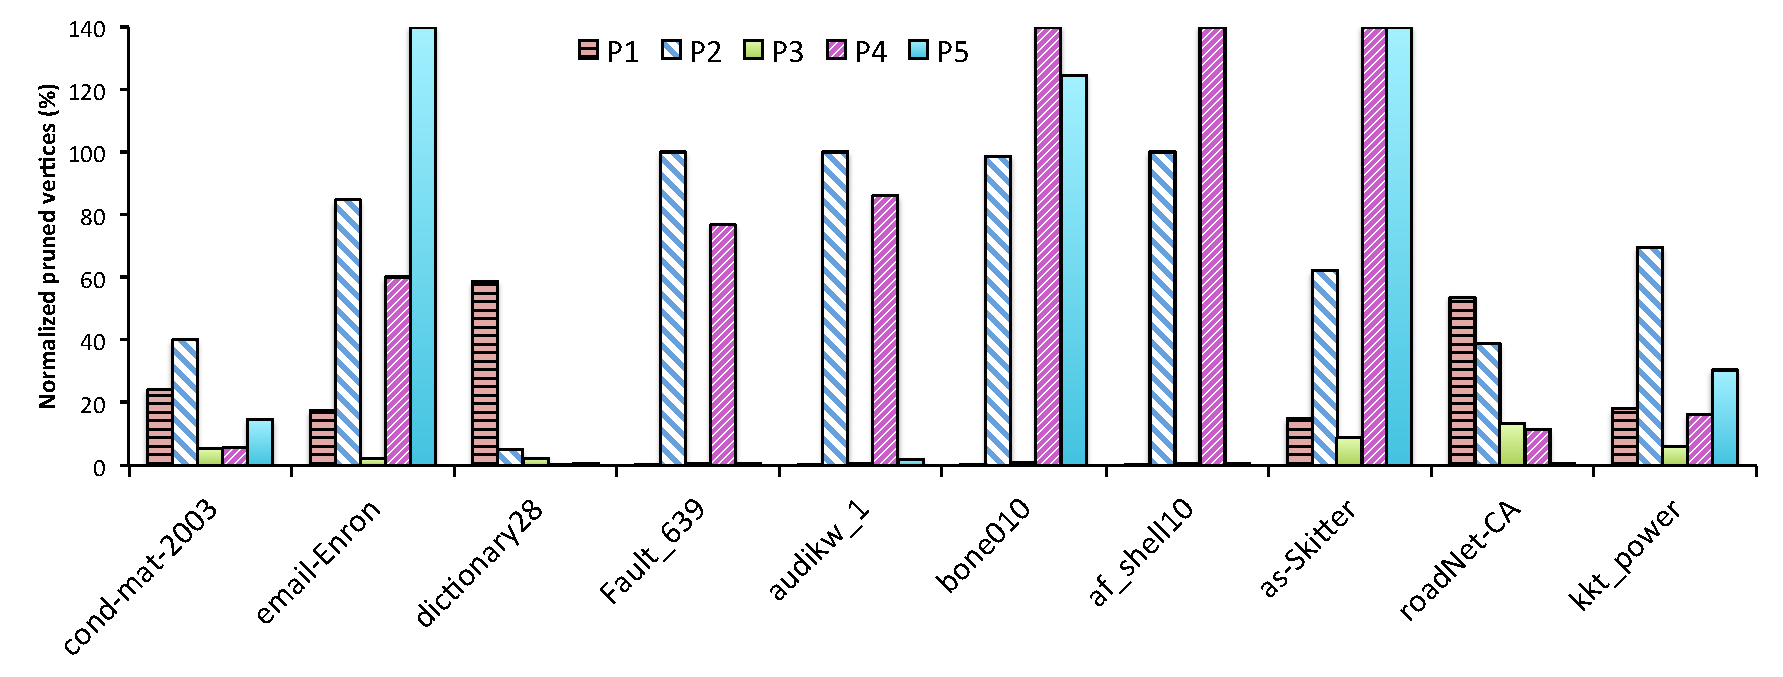
\includegraphics[scale=0.5]{pruned.pdf}
\caption{Number of ``pruned" vertices in the various pruning steps normalized
by the number of edges in the graph (in percents) for the test graphs in category 1 (we cut few bars reachining 140\% as their correspnding values are much higher).}
\label{fig-pruningplot}
\end{figure}


In Figure~\ref{fig-pruningplot} we show the number of vertices discarded by all
the  pruning steps of the exact algorithm normalized by the total number of edges
in a graph for the real-world graphs (category 1) in the testbed. We cut few bars reachining
140\% as their correspnding values are much higher.
In the Appendix, we provide a complete tabulation of the raw numbers for the pruned vertices in all the steps for all the graphs in the testbed. It can be seen for these graphs pruning steps 2 and 5 in particular discard a large percentage of vertices, potentially resulting in large runtime savings. The general behavior of the pruning steps Pruning 1, 2, 3 and 5 for the synthetic graphs {\em rmat\_er} and {\em rmat\_sd1} was observed to be somewhat similar to that depicted in Figure~\ref{fig-pruningplot} for the real-world graphs. In contrast, for the DIMACS graphs, the number of vertices pruned in steps Pruning 1, 3 and 5 were observed to be zero; the numbers in the step Pruning 2 were nonzero but relatively modest.
%Since our new pruning steps hierarchically reduce the search space, one can expect a decreasing order of effect in the performance of Prunings 1, 2, 3 and 5, with Pruning 1 having the highest impact, and 5 the lowest. 


As a result  of the differences seen in the effects of the pruning steps, as discussed below,
the runtime performance of our algorithm (seen in Table \ref{tab:timings}) compared
to the other three algorithms varied in accordance with the difference in the structures represented 
by the different categories of graphs in the testbed.

{\bf Real-world Graphs. }
For most of the graphs in this category, it can be seen that our algorithm runs several orders of magnitude faster than the other three, mainly due to the large amount of pruning the algorithm attained. These numbers also illustrate the great benefit of hierarchical pruning. 
For the graphs {\em Fault\_639}, {\em audikw\_1} and {\em af\_shell10}, 
Prunings 1, 3 and 5 have only minimal impact,
whereas Pruning 2 makes a big difference resulting in impressive runtimes. 
The number of vertices pruned in steps Pruning 1 and 3 varied among the 
graph {\em within} the
category, ranging from 0.001\% for {\it af\_shell} to a staggering 97\% for {\it as-Skitter} 
for the step Pruning 1. 
%We observe that the relative speedup factor of our algorithm is the highest for
%the graphs with high maximum clique size and high maximum degree.
%as well. For instance, for as-Skitter reduction the search space is reduced dramatically due to pruning, and results in a very impressive performance.



{\bf Synthetic Graphs. }
For the synthetic graph types {\it rmat\_er} and {\it rmat\_sd1}, our algorithm clearly outperforms 
the other three by a few orders of magnitude in all cases. 
This is also primary due to the high number of vertices discarded by the new pruning steps. 
In particular, for {\it rmat\_sd1} graphs, between 30 to 37\% of the vertices are pruned just in the step Pruning 1. 
%The {\it rmat\_er} and the corresponding {\it rmat\_sd1} graphs have nearly equal number of vertices and edges, however, the timings of the {\it rmat\_er} graphs are relatively better because of the smaller size of the maximum clique and the smaller maximum degree. 
For the {\it rmat\_sd2} graphs, which have relatively larger maximum clique and higher maximum degree than the {\it rmat\_sd1} graphs, our algorithm is observed to be faster than 
CP but slower than {\em cliquer}. 

{\bf DIMACS Graphs. }
The runtime of our exact algorithm for the DIMACS graphs is 
in most cases comparable to that of CP and higher than that of {\it cliquer}
and {\it MCQD+CS}.
%As can be seen from the Table  \ref{tab:timings}, 
For these graphs, only Pruning 2 was found to be effective, 
and thus the performance results agree with one's expectation. 
%We include in the Appendix timing results on a larger collection of DIMACS graphs. 



It is to be noted that the DIMACS graphs are intended to serve as challenging test cases for the maximum clique problem, and graphs with such high edge densities and low vertex count are rare in practice. 
Most of these have between 20 to 1024 vertices with an average edge density of roughly 0.6, 
whereas, most real world graphs are often very large and sparse
as exemplified by the real-world graphs in our test bed.
Other good examples of instances with similar nature include Internet topology graphs \cite{Faloutsos:1999:PRI:316188.316229}, the web graph \cite{kumar:extracting}, and social network graphs \cite{Domingos:2001:MNV:502512.502525}.


%\vspace{-15pt}
\subsubsection{The Heuristic}
\label{sec:exp-heuristic}

It can be seen that our heuristic runs several orders of magnitude faster than our exact algorithm,
while delivering either optimal or very close to optimal solution.
It gave the optimal solution on 25 out of the 30 test cases.
On the remaining 5 cases where it was suboptimal, its accuracy ranges from 83\% to 99\% (on average 93\%).

Additionally, we run the heuristic by choosing a vertex randomly in Line \ref{maxDsel} of Algorithm \ref{alg:mClqHeu} instead of the one with the maximum degree. We observe that on average, the solution is optimal only for less than $40\%$ of the test cases compared to 83\% when selecting the maximum degree vertex.
%after three repetitions with different random seeds


\begin{SCfigure}
  \centering
    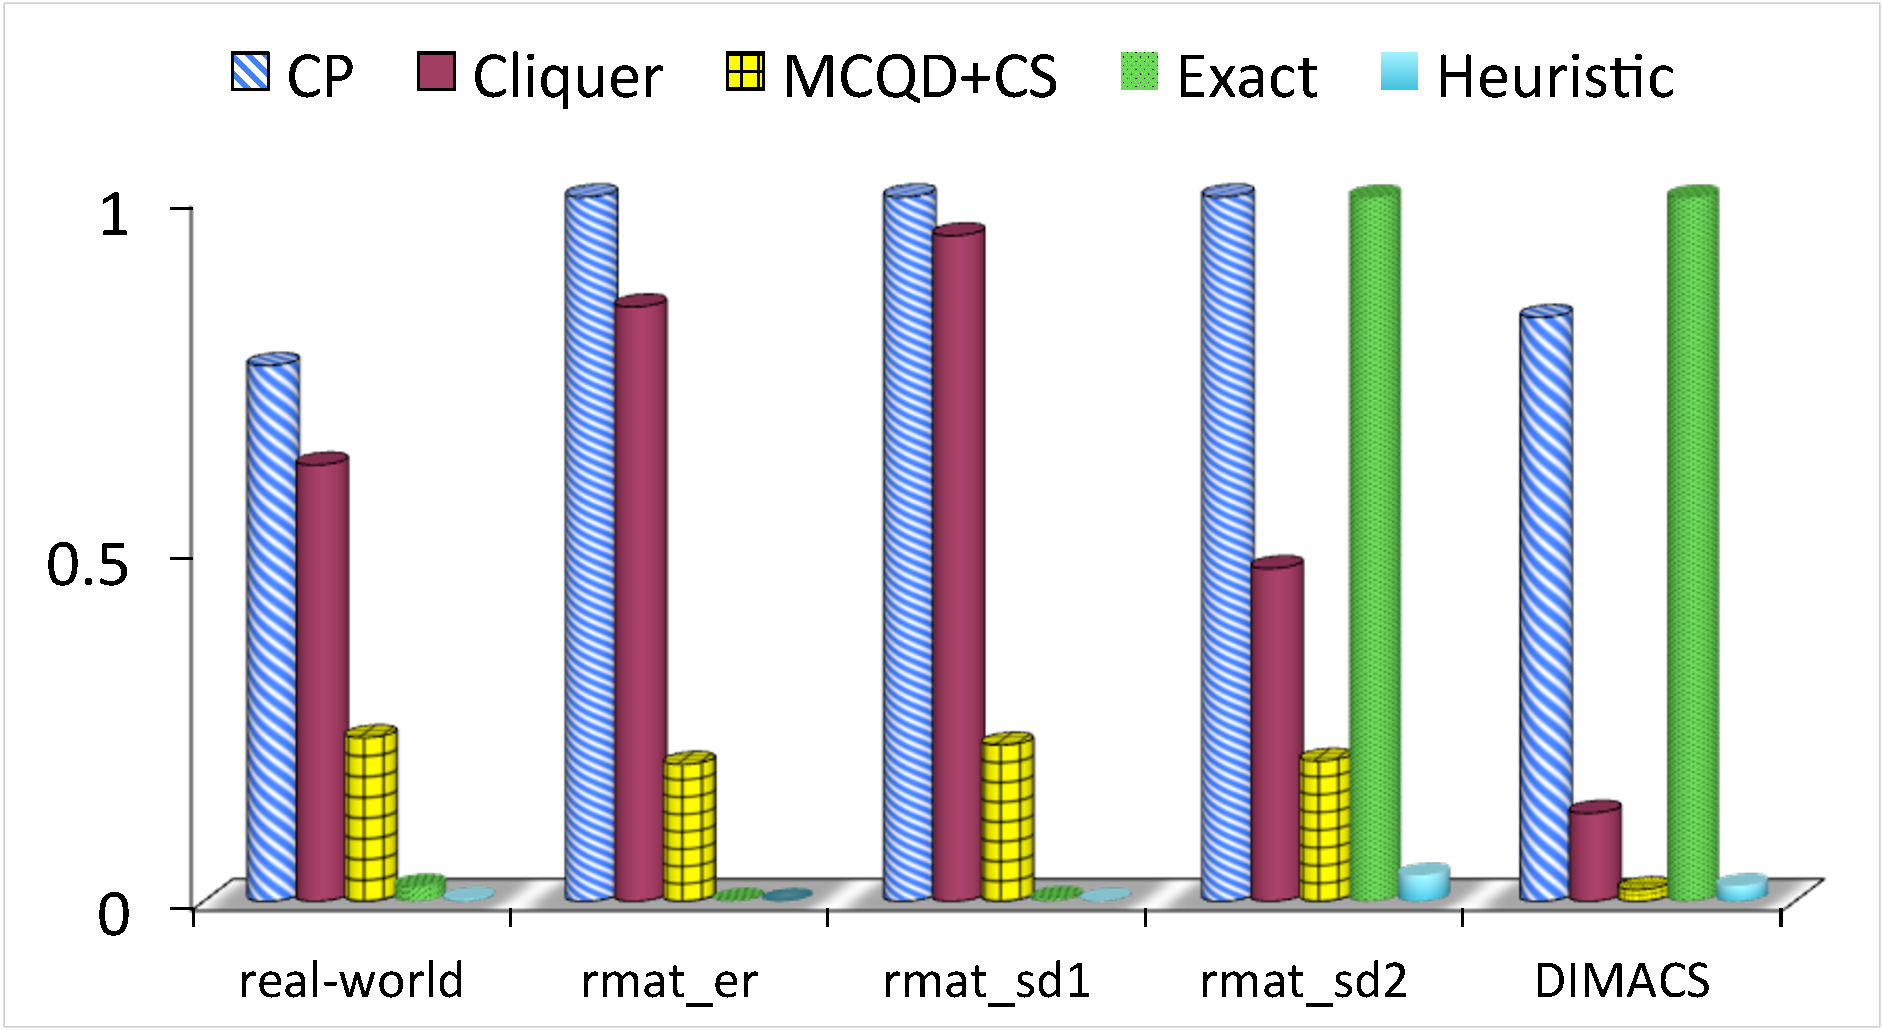
\includegraphics[width=7.8cm]{maxclqplot.pdf}
%%\vspace{-30pt}
  \caption{Runtime (normalized, mean) comparison between various algorithms. For each category of graph, first, all runtimes for each graph were normalized by the runtime of the slowest algorithm for that graph, and then the mean was calculated for each algorithm. Graphs were considered only if the runtimes for at least three algorithms was less than the 25,000 seconds limit set.}
\label{fig-timeplot}
\end{SCfigure}
%\vspace{-10pt}
%\vspace{-10pt}




\subsubsection{Further Analysis}
\label{sec:exp-further}

Figure~\ref{fig-timeplot} provides an aggregated visual summary of the runtime trends of
the various algorithms across the five categories of graphs in the testbed. 
%The bars in each category
%are created as follows. First the runtime for each algorithm for each graph in a category is divided by the runtime of the slowest algorithm for that graph. Then the mean of these is taken as a resut for the category. Values enter into the mean calculation when runtimes are available for
%at least three algorithms.


To give a sense of runtime growth rates, we provide in Figure~\ref{fig-runtimeplots} plots of the 
runtime of the new exact algorithm and the heuristic for the synthetic and real-world graphs 
in the testbed. In addition to the curves corresponding to the runtimes of the
{\em exact} algorithm and the {\em heuristic}, the figures also include a curve corresponding to
the number of {\em edges} in the graph divided by the clock frequency of the computing
platform used in the experiment. This curve is added to facilitate comparison between
the growth rate of the runtime of the algorithms with that of a linear-time (in the size of the graph) growth rate. 
It can be seen that the runtime of the heuristic by and large grows 
somewhat linearly with the size of a graph. The exact algorithm's runtime, which is orders of
magnitude larger than the heuristic, exhibited a similar growth behavior for these test-cases
even though its worst-case complexity suggests exponential growth in the general case. 


\begin{figure}
  \centering
    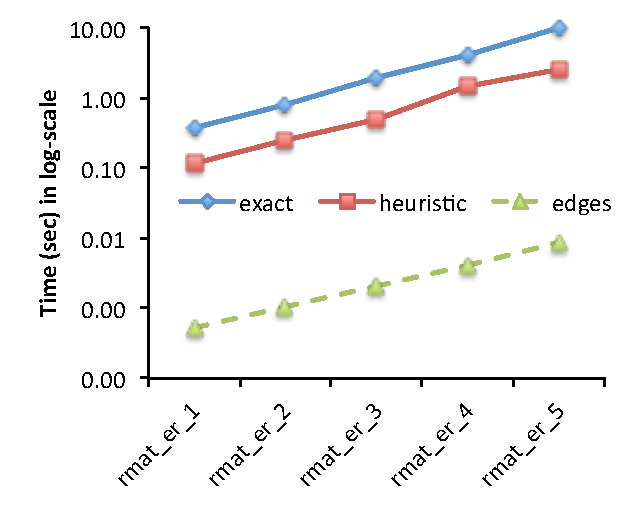
\includegraphics[scale=0.67]{compare_time_er.pdf}
    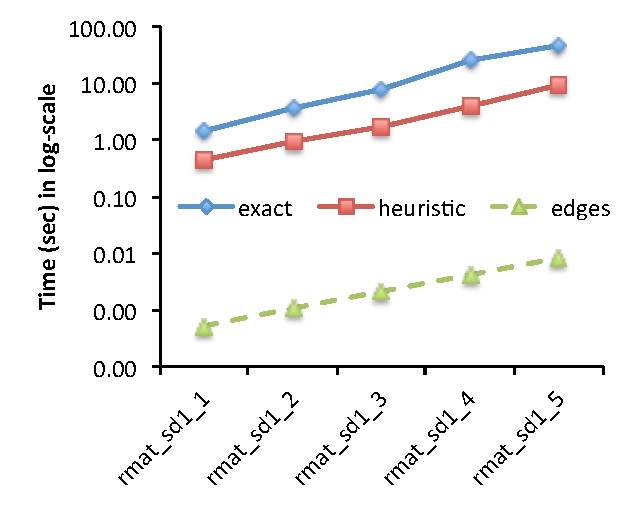
\includegraphics[scale=0.67]{compare_time_sd1.pdf}\\
    
    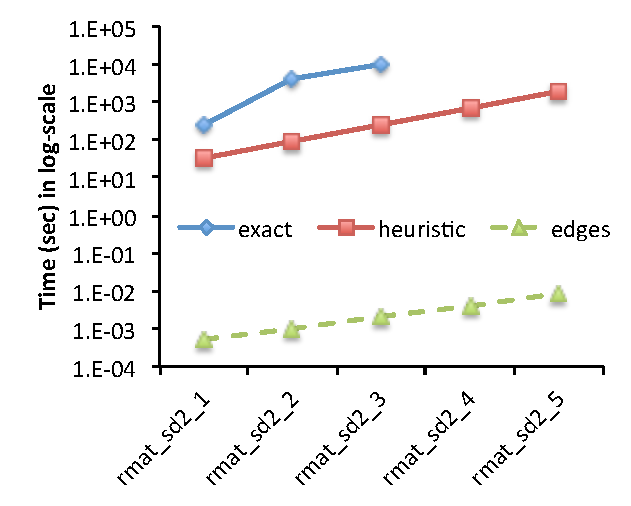
\includegraphics[scale=0.67]{compare_time_sd2.pdf}
    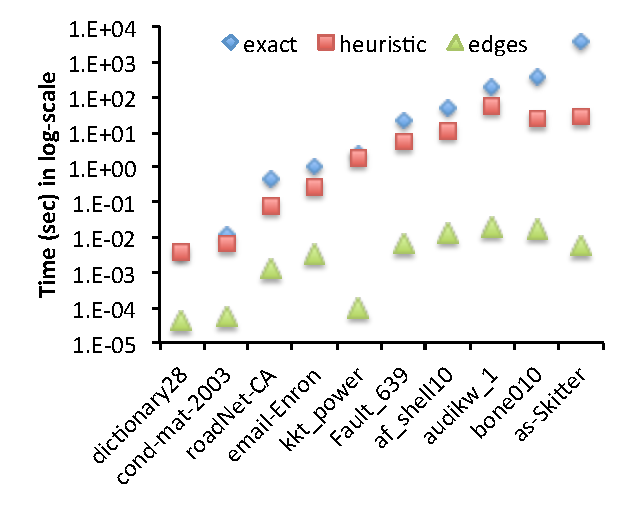
\includegraphics[scale=0.67]{compare_time_rw.pdf}
    
%%\vspace{-30pt}
 \caption{Run time plots of the new exact and heuristic algorithms. The third curve, labeled
 {\em edges}, shows the quantity number of edges in the graph divided by the clock 
 frequency of the computing platform used in the experiment. 
 }
\label{fig-runtimeplots}
\end{figure}



%Finally, we comment on our experience in using the 
%{\it MaxCliqueDyn} code.
%Unfortunately, the code failed to execute most of the  
%large instances in our testbed, including the majority of the RMAT and real-world instances,
%due to memory management issues in the code. 
%The entries in Table~\ref{tab:timings} marked with hyphen (-) show instances
%for which the code crashed.
%One of the few instance we were able to successfully run was {\it email-enron}.
%For it, the code took 4.91 seconds to compute the maximum clique 
%(using the same experimental setup), whereas our algorithm took only 0.998 seconds. 
%The memory issue also prevented us from do an extensive comparison with the other more recent algorithms 
%based on \cite{citeulike:7905505} and including \cite{Tomita:2007:EBA:1188122.1188130}, 
%since to our knowledge, there does not exist any other publicly available package 
%based on this algorithm. 
%On a related note, our attempts to run instances larger than the ones used in the experiments reported here on the
%the {\em cliquer}  package (\url{http://users.tkk.fi/pat/cliquer.html} \cite{cliquer}) failed because of similar memory leak issues. 
%This makes our code (available at \url{http://cucis.ece.northwestern.edu/projects/MAXCLIQUE/}) the only open source code,
%which has been tested to be capable of finding the maximum clique of large instances. Note that our code also
%includes a converter between two popular graph formats, DIMACS to/from matrix market.
%Even for the instances it eventually run successfully, we had to first make modifications to the graph reader
%to make it able to handle graphs with multiple connected components.
%{\it 
%The fixes and related discussion I had to do in the available source code of MaxCliqueDyn \cite{konc2007improved} is as follows:
%The graph reader fails to read large graphs specially when the graph contains disjoint vertices. 
%The reader tries to allocate memory based on the number of distinct vertices and it 
%assumes the number of vertices is equal to the number of distinct vertices (which could be much lower) as the package
%has mostly been developed keeping the densed small graphs in mind. 
%Because of this there code can't run for the massive sparse graphs as the vertex ID becomes higher
%than the number of vertices and therefore access invalid memory locations and gives segmentation fault.
%I guess the reason they do this is to reduce the required memory by the algorithm (as the reply from the author says,
%at every round it allocates memory equal to the number of vertices, and therefore eventually the expected space requirement
%could be O($n^2$)). We therefore fixed the problem 
%by disallowing the code to change the number of vertices to the number of dictinct vertices.
%After doing this we noticed that the reader is capable of loading larger sparse graphs, but the algorithm runs 
%for long time and incrementally asks huge memory and the job become killed at some point
%For example, we noticed when we run experiment on $Fault$ graph, its being killed when
%the allocated memory reaches 100 GB.
%}

%\subsection{Example of an application in social network analysis}
\label{sec:applications}

We conclude this section on experiments with a small example 
demonstrating the application of the clique algorithms for detecting overlapping communities in social networks. 
In many real networks vertices may belong to more than one group, and such groups form overlapping communities. Classical examples are social networks, where an individual usually belongs to different circles at the same time, from that of work colleagues to family, sport associations, etc. 
Finding overlapping communities is a challenging problem \cite{Fortunato_2010}.
Clique algorithms are one way in which a solution can be found.  
%A detailed overview of community detection methods, and the significance and complexity involved in overlapping community findingcan be found in \cite{Fortunato_2010}.

%\vspace{-20pt}
\begin{figure}%[h!]
  \centering
    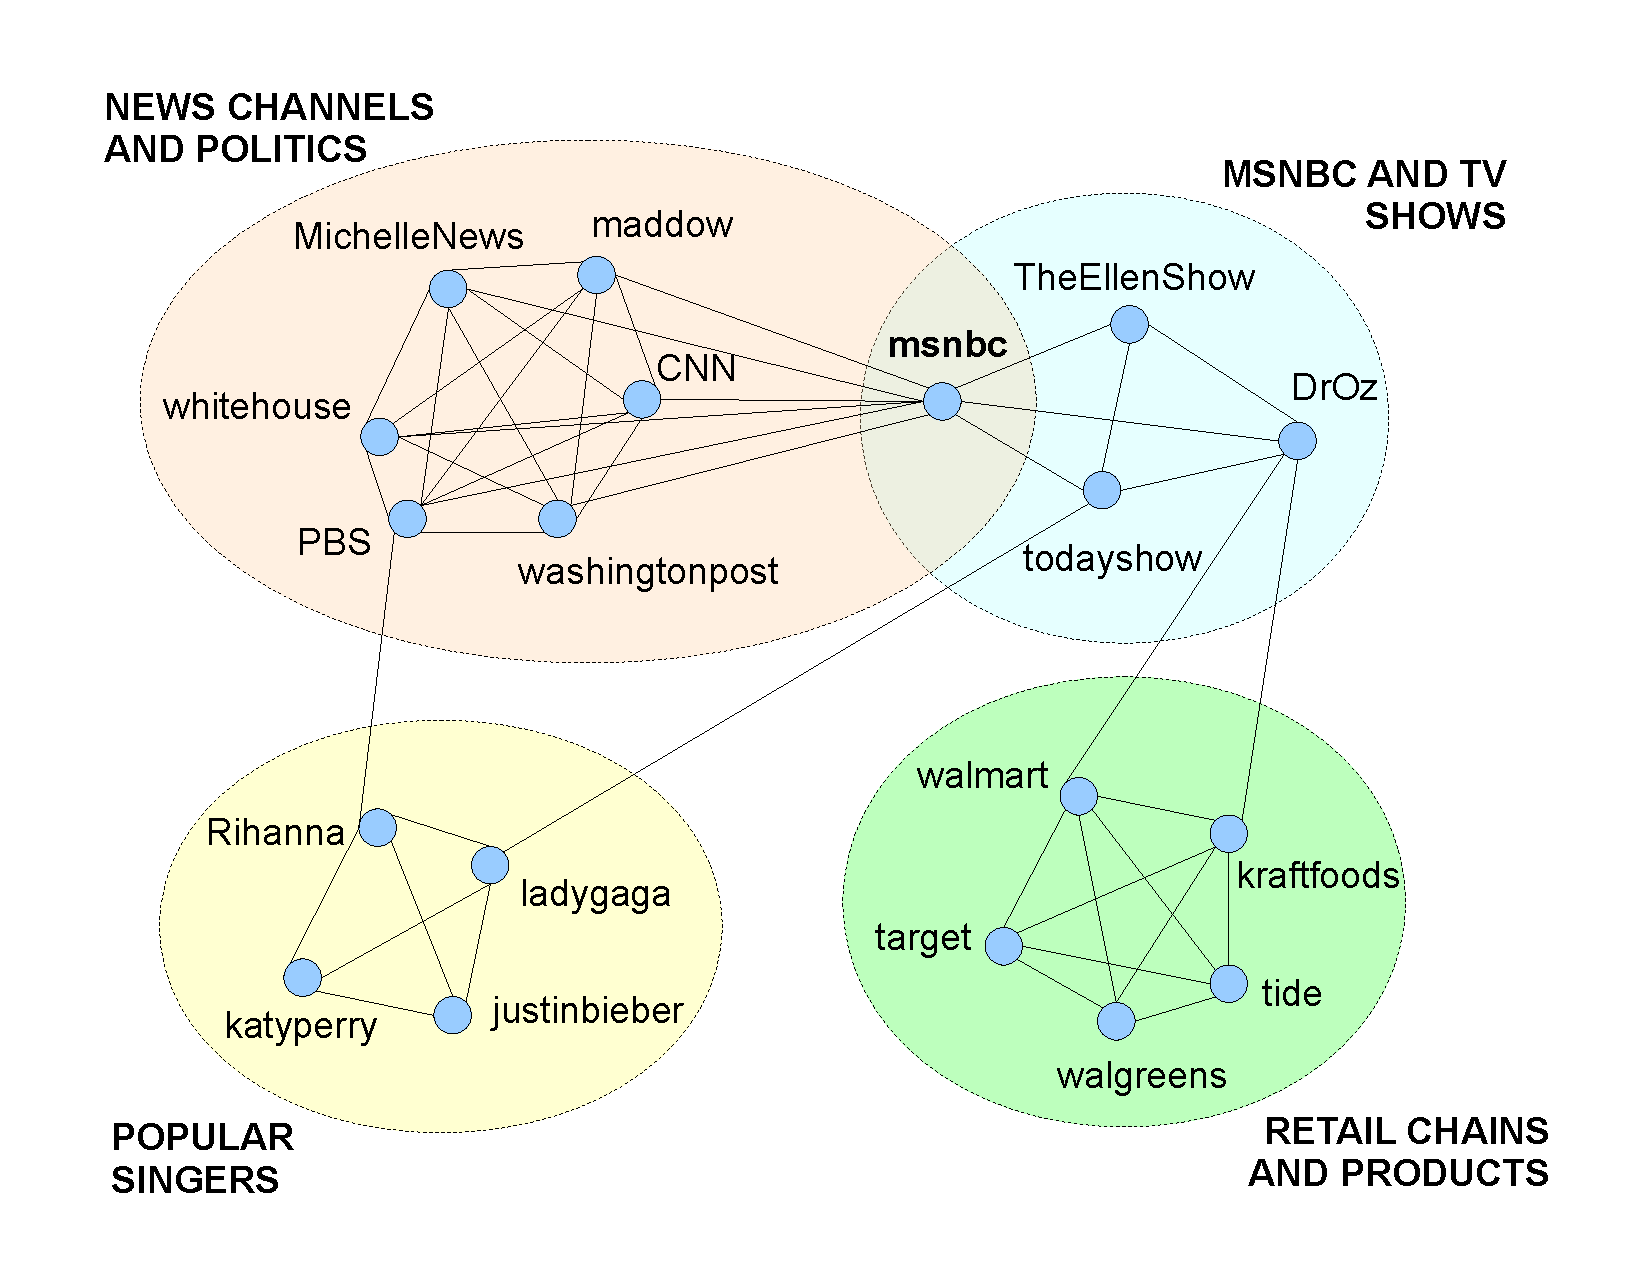
\includegraphics[width=1\textwidth]{communities.pdf}
%\vspace{-30pt}
  \caption{Some Facebook communities detected by our max clique heuristic.}
\label{fig-communities}
\end{figure}
%\vspace{-10pt}

%\footnotetext{http://www.facebook.com}
For our small experiment, we use data collected from Facebook\footnote[1]{http://www.facebook.com}.
Every user on Facebook has a {\it wall}, which is a the user's profile space that allows the posting of messages, often short or temporal notes by other users. The user comments and user information from specific {\it walls} are publicly available and we collected them using Facebook API. We constructed a graph with the {\it walls} as vertices. Any two users who have commented on the same {\it wall} indicate a connection between the {\it walls}, and we form an edge between them. There could be many common users for each wall, and so we assigned edge weights by Jacard index or similarity coefficient \cite{Leydesdorff}. Once this is done for all {\it walls}, we retained only those edges which have weights above a chosen threshold, indicating a strong correlation. The threshold is a user's choice and decides both the size and the number of communities found.
% If an edge already exists, we increase the edge weight by 1. Once this is done for all {\it walls}, the edge weights are normalized, and we retain only those edges which have edge weights above a chosen threshold (we use 0.01), indicating a strong correlation.

%duplicate removal
We modified our heuristic to retain the largest maximum clique containing each node. 
%This is done by simply substituting Lines 3 and 4 of Algorithm \ref{alg:clqHeu}, with a simple routine that stores each clique in a preferred data structure. 
The exact algorithm could have also been used instead of the heuristic for this purpose. We choose the heuristic since it is much faster and for this particular problem of community detection the accuracy of the size of cliques formed is not critical.

Figure \ref{fig-communities} shows some of the cliques/communities detected. We see two isolated communities, one for popular singers, and another for retail chains and products. We also see a community for news channels and politics, and a community of MSNBC and popular TV shows. The highlight of this experiment  is that the
clique algorithm allows a node to be a member of more than one community giving an overlapping community structure. Although the {\it news channels and politics} and {\it MSNBC and tv shows} communities are not directly related and have different members, they share a common member.
%add from nature paper why this is significant. coexistence of their structural subunits 



%\vspace{-10pt}

\section{Parallelization}
\label{sec:parallelization}

%The ease with which an algorithm can be parallelized and its performance is important for handling large-scale graphs in emerging applications, where graphs with millions (or more) vertices have become quite common. 

 We describe in this section how our exact algorithm can be parallelized and show performance results
on a shared-memory platform. The heuristic can be parallelized following a similar procedure.

%We here describe the parallelization procedure for both shared and distributed memory architecture. 
As explained in Section \ref{sec:algorithms}, the $i$th iteration of the {\em for} loop in the exact algorithm computes the size of the largest clique that contains the vertex $v_i$. Since our algorithm doesn't require a specific order in which vertices have to be processed, these iterations can in principle be performed concurrently. In such a concurrent computation, however, different processes might discover current maximum cliques of different sizes---and 
for the pruning steps to be most effective, the current globally largest maximum clique size needs to be communicated to all processes as soon as it is discovered. In a shared-memory programming model, the global maximum clique size can be stored as a shared variable accessible to all the processing units, and its value can be updated by the relevant processor at any given time. In a distributed-memory setting more care needs to be exercised to keep the communication cost low. 
%For the distributed case, the effects of pruning could, however, be tolerably compromised in order to enable the parallel computation. This can, for example, be done by using the most recent value of the maximum clique size for pruning, and updating this value by having synchronization steps at regular intervals.

We implemented a shared-memory parallelization based on the procedure described above using OpenMP. Since the global value of the maximum clique is shared by all processing units, we embed the updating of the maximum clique, i.e. Line \ref{critical} of Algorithm \ref{alg:mClq}, in a {\it critical} section (an OpenMP feature that enforces a lock allowing only one thread to make the update at a time). Further, we used  dynamic load scheduling, since different vertices might return different sizes of maximum clique resulting in different work loads.
%, so would work best for our case.

We performed experiments on the same graphs listed in the testbed described in Section \ref{sec:experiments}. For these, we used a Linux workstation 
%running 64-bit version Red Hat Enterprise Linux Server release 6.2 
with six 2.00 GHz Intel Xeon E7540 processors. Each processor has six cores, each with 32 KB of L1 and 256 KB of L2 cache, and each processor shares an 18 MB L3 cache.  
%Implementation was in C++ using OpenMP and compiled with gcc (version 4.4.7) using the -O3 optimization flag.


\begin{figure}
  \centering
    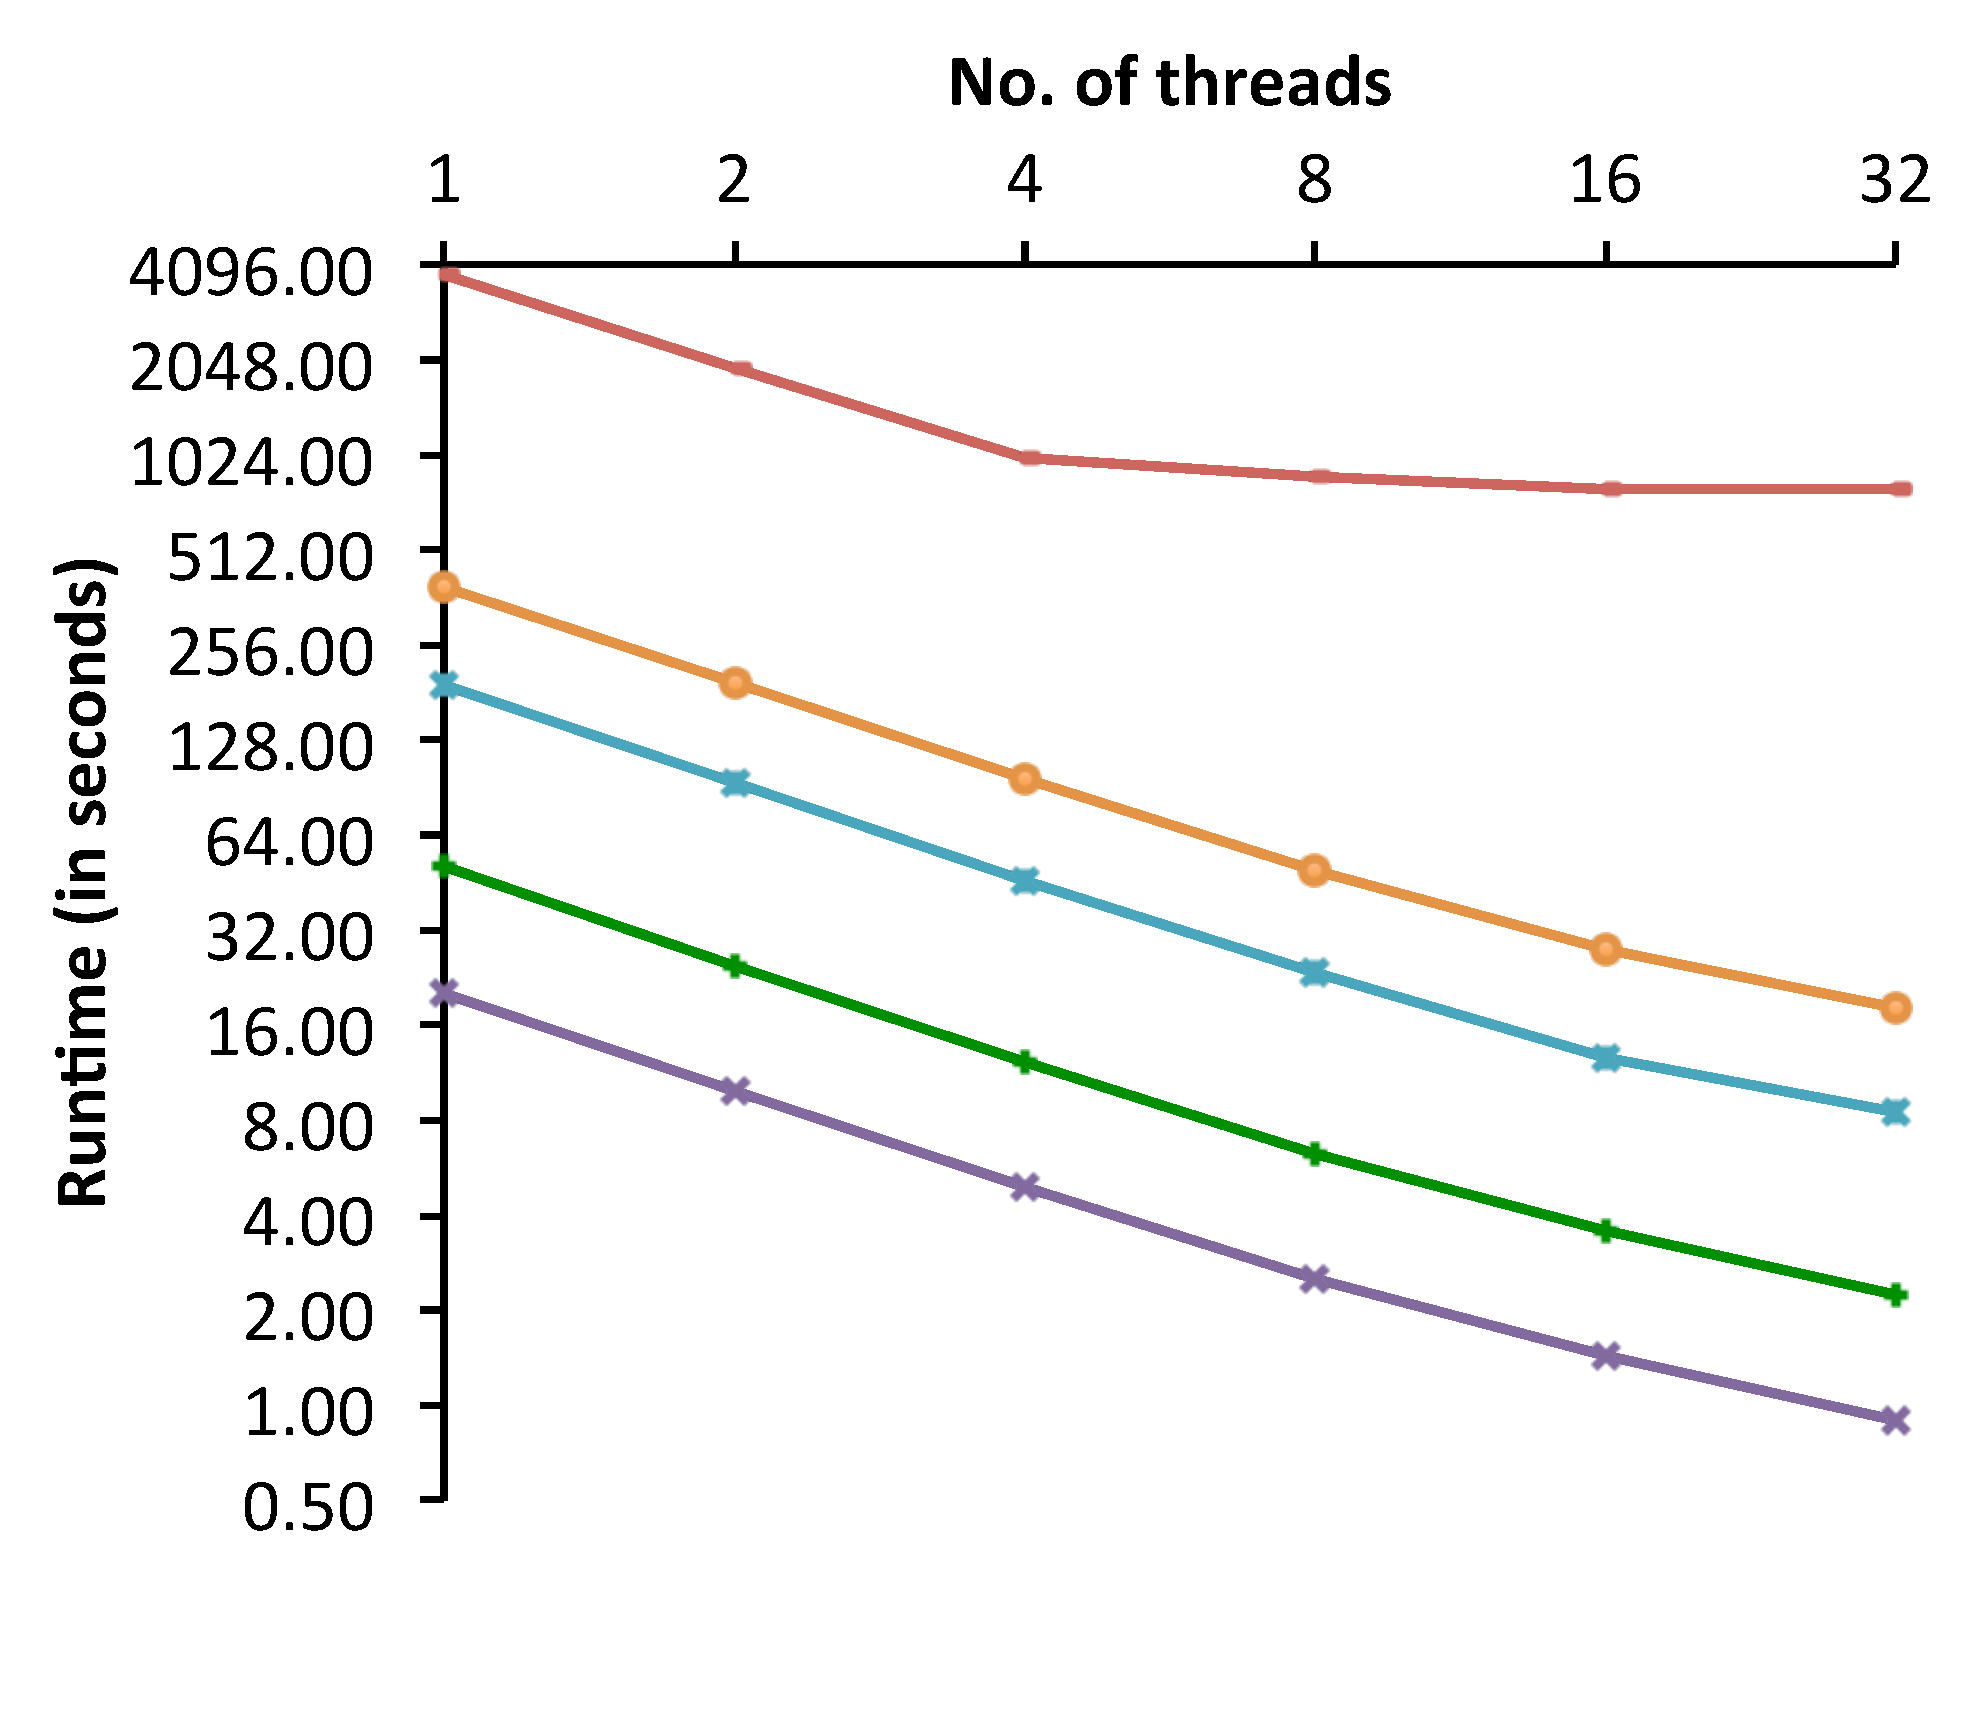
\includegraphics[scale=0.17]{parallel_realworld_timing.pdf}
    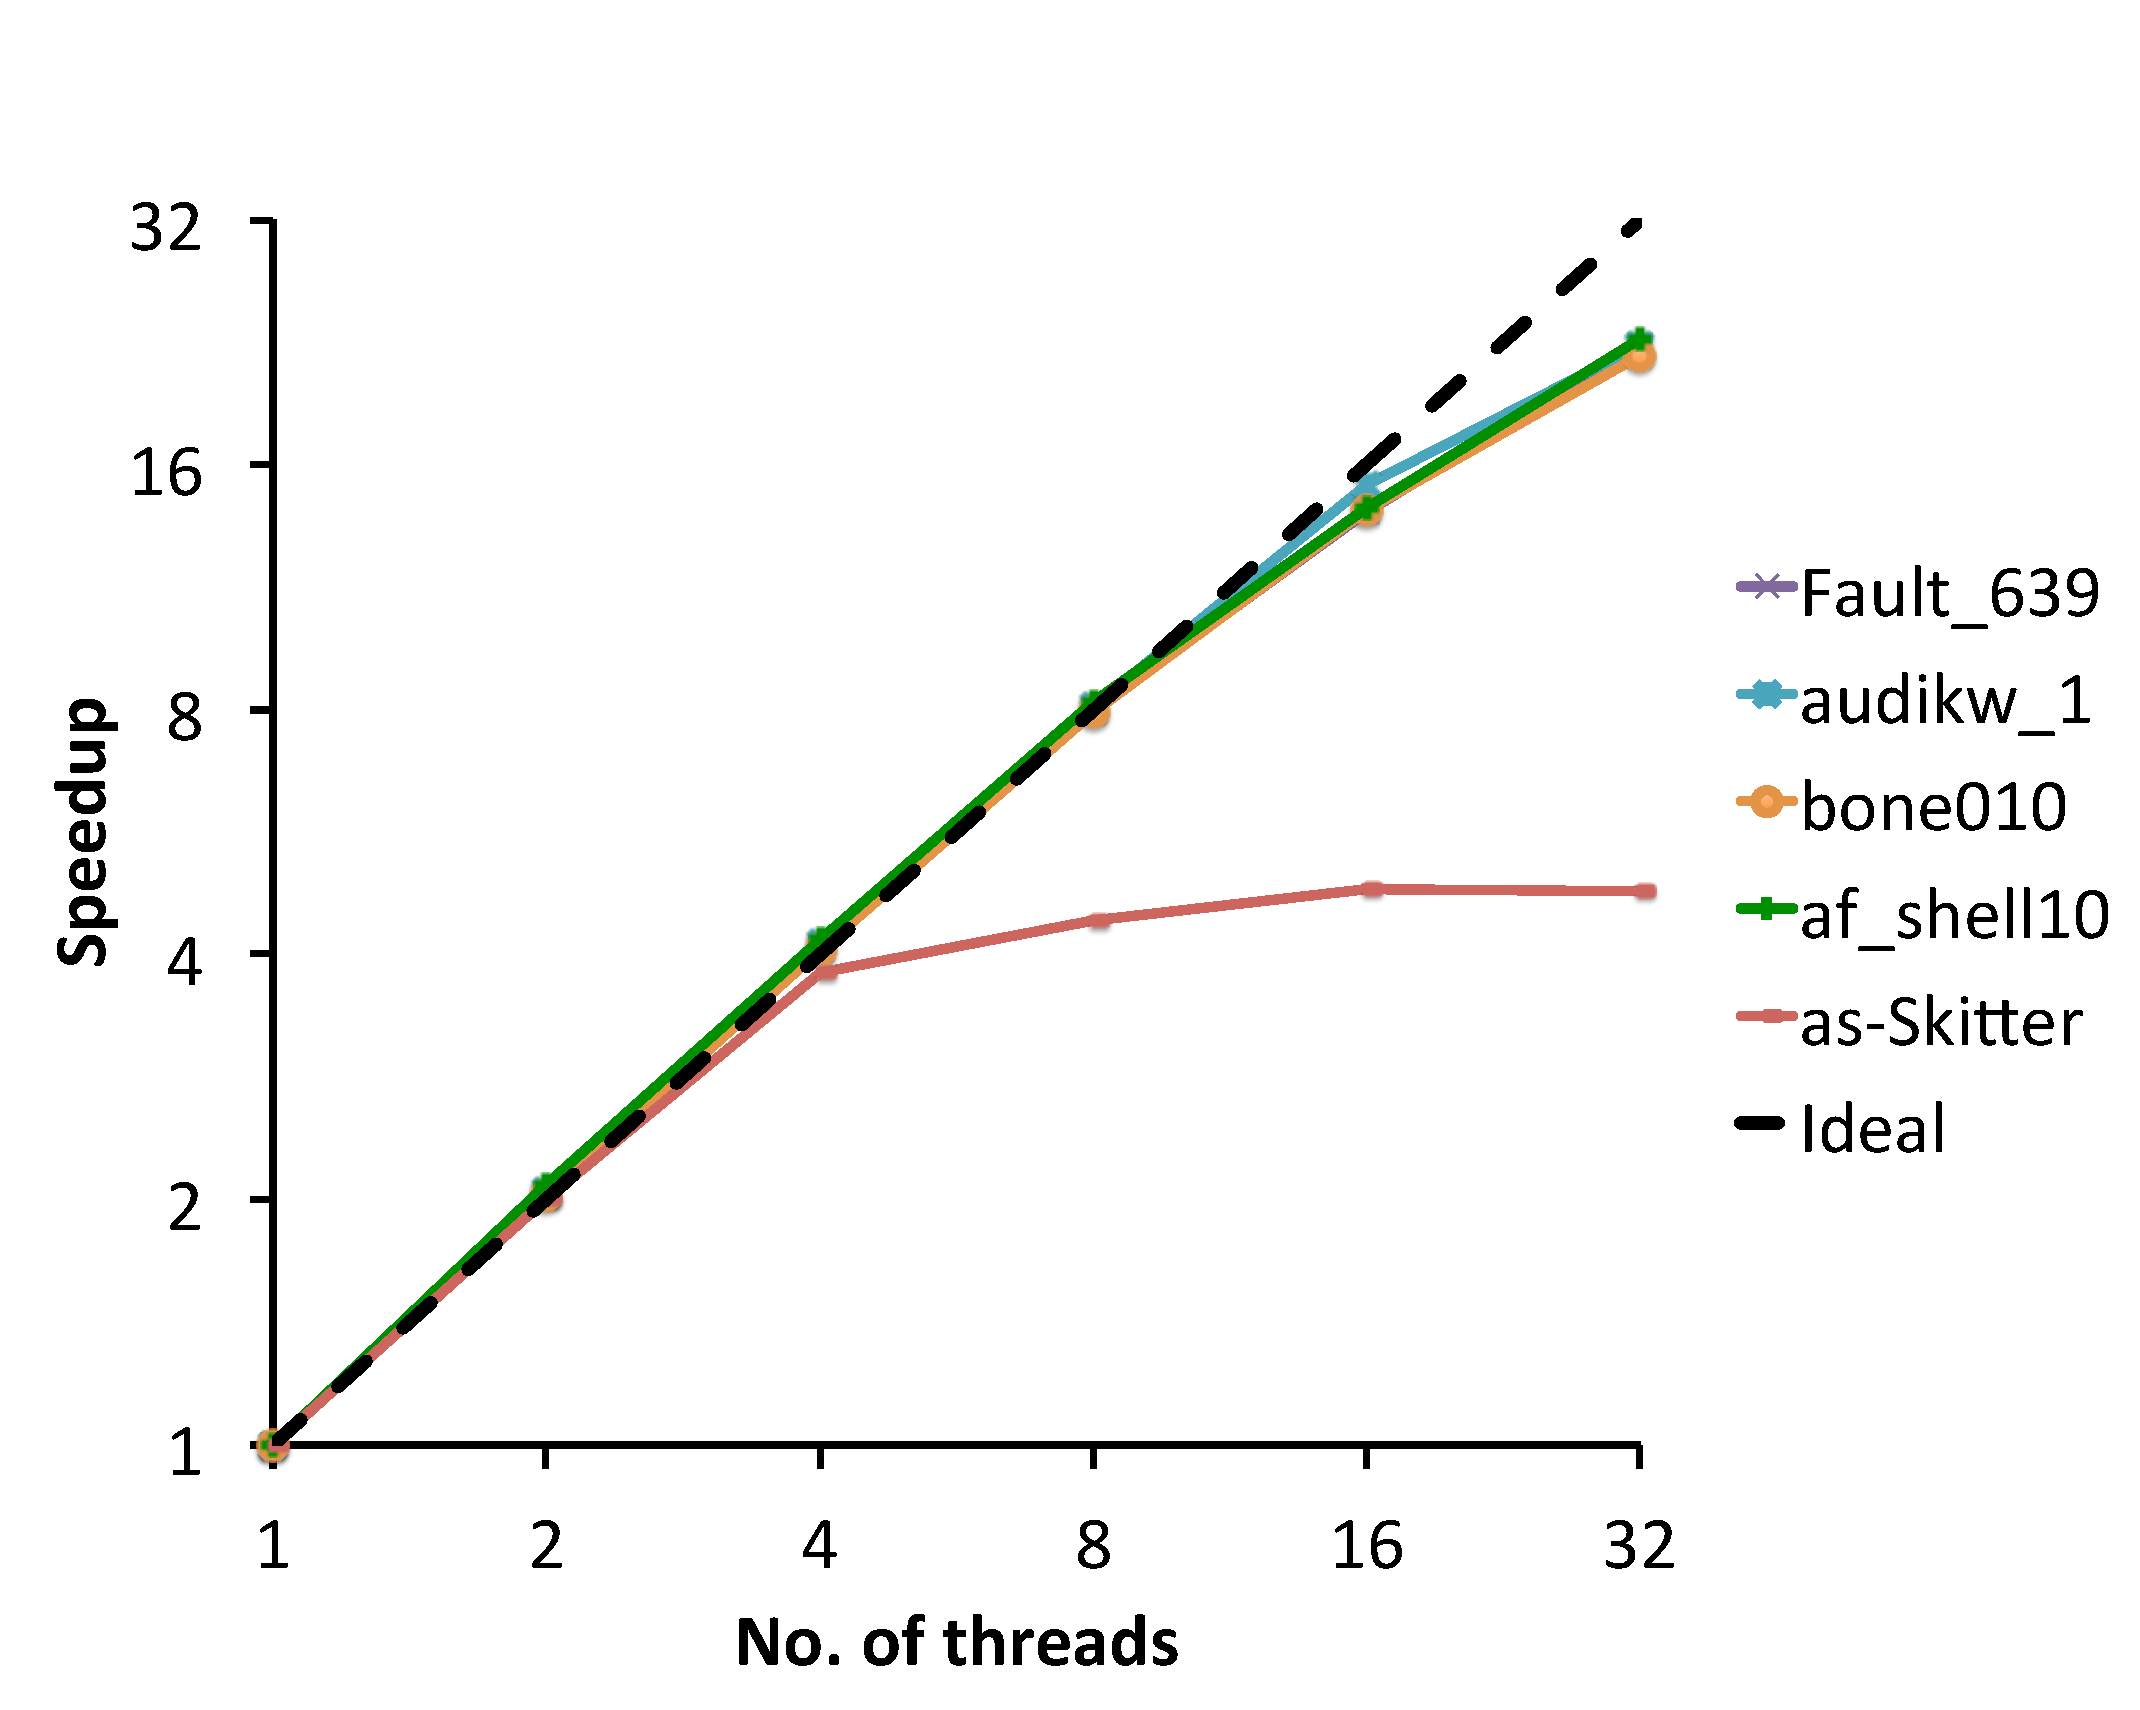
\includegraphics[scale=0.17]{parallel_realworld_speedup.pdf}
    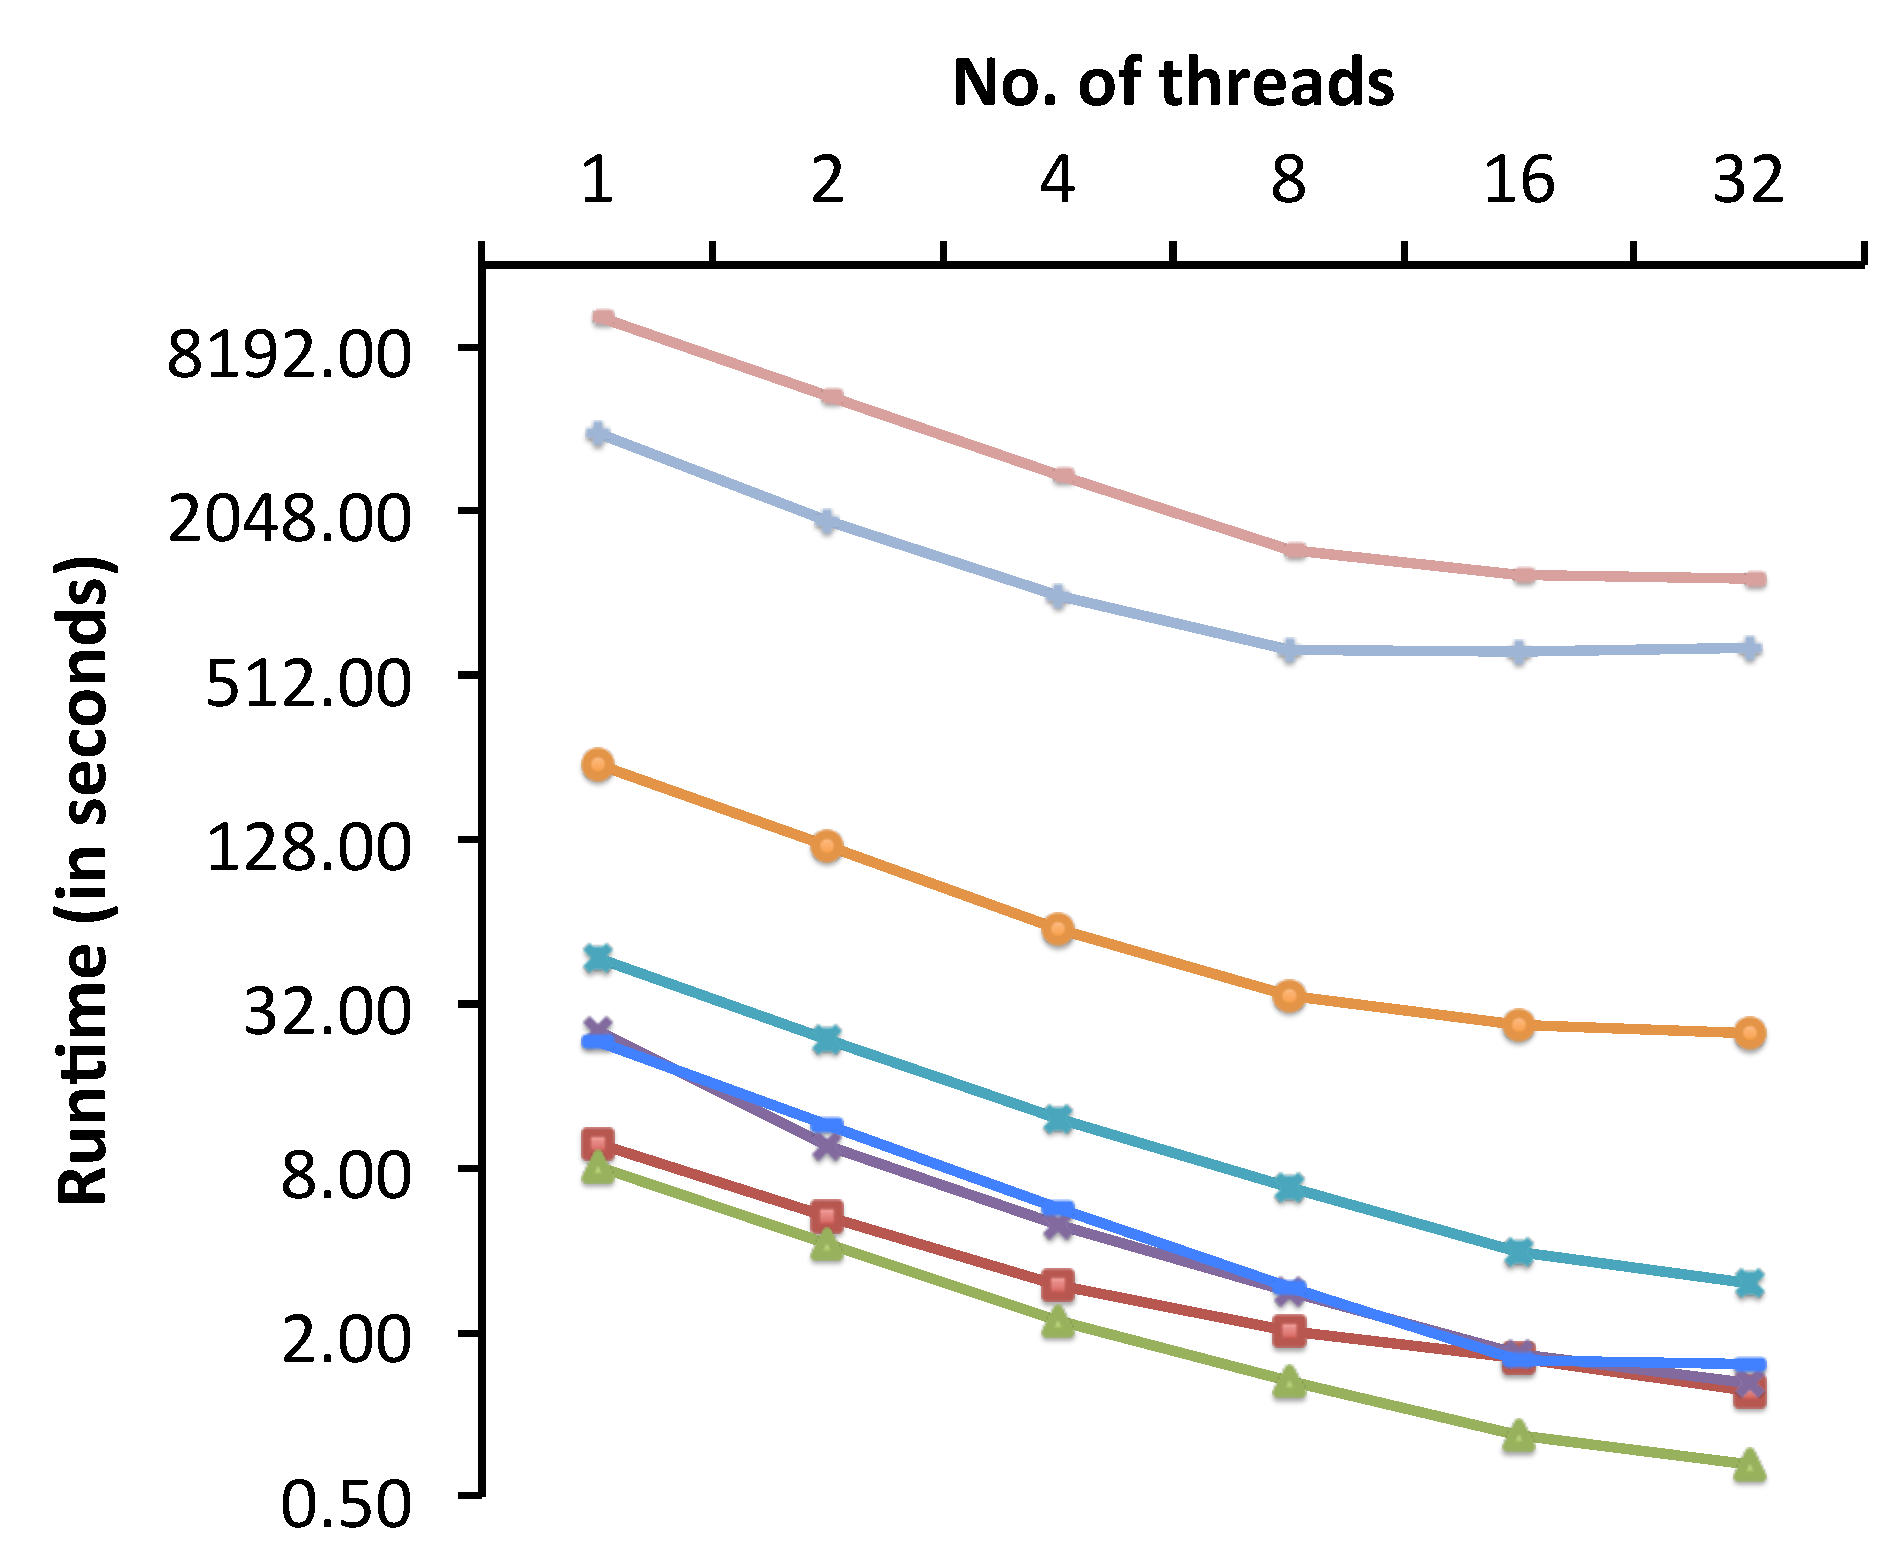
\includegraphics[scale=0.17]{parallel_other_timing.pdf}
    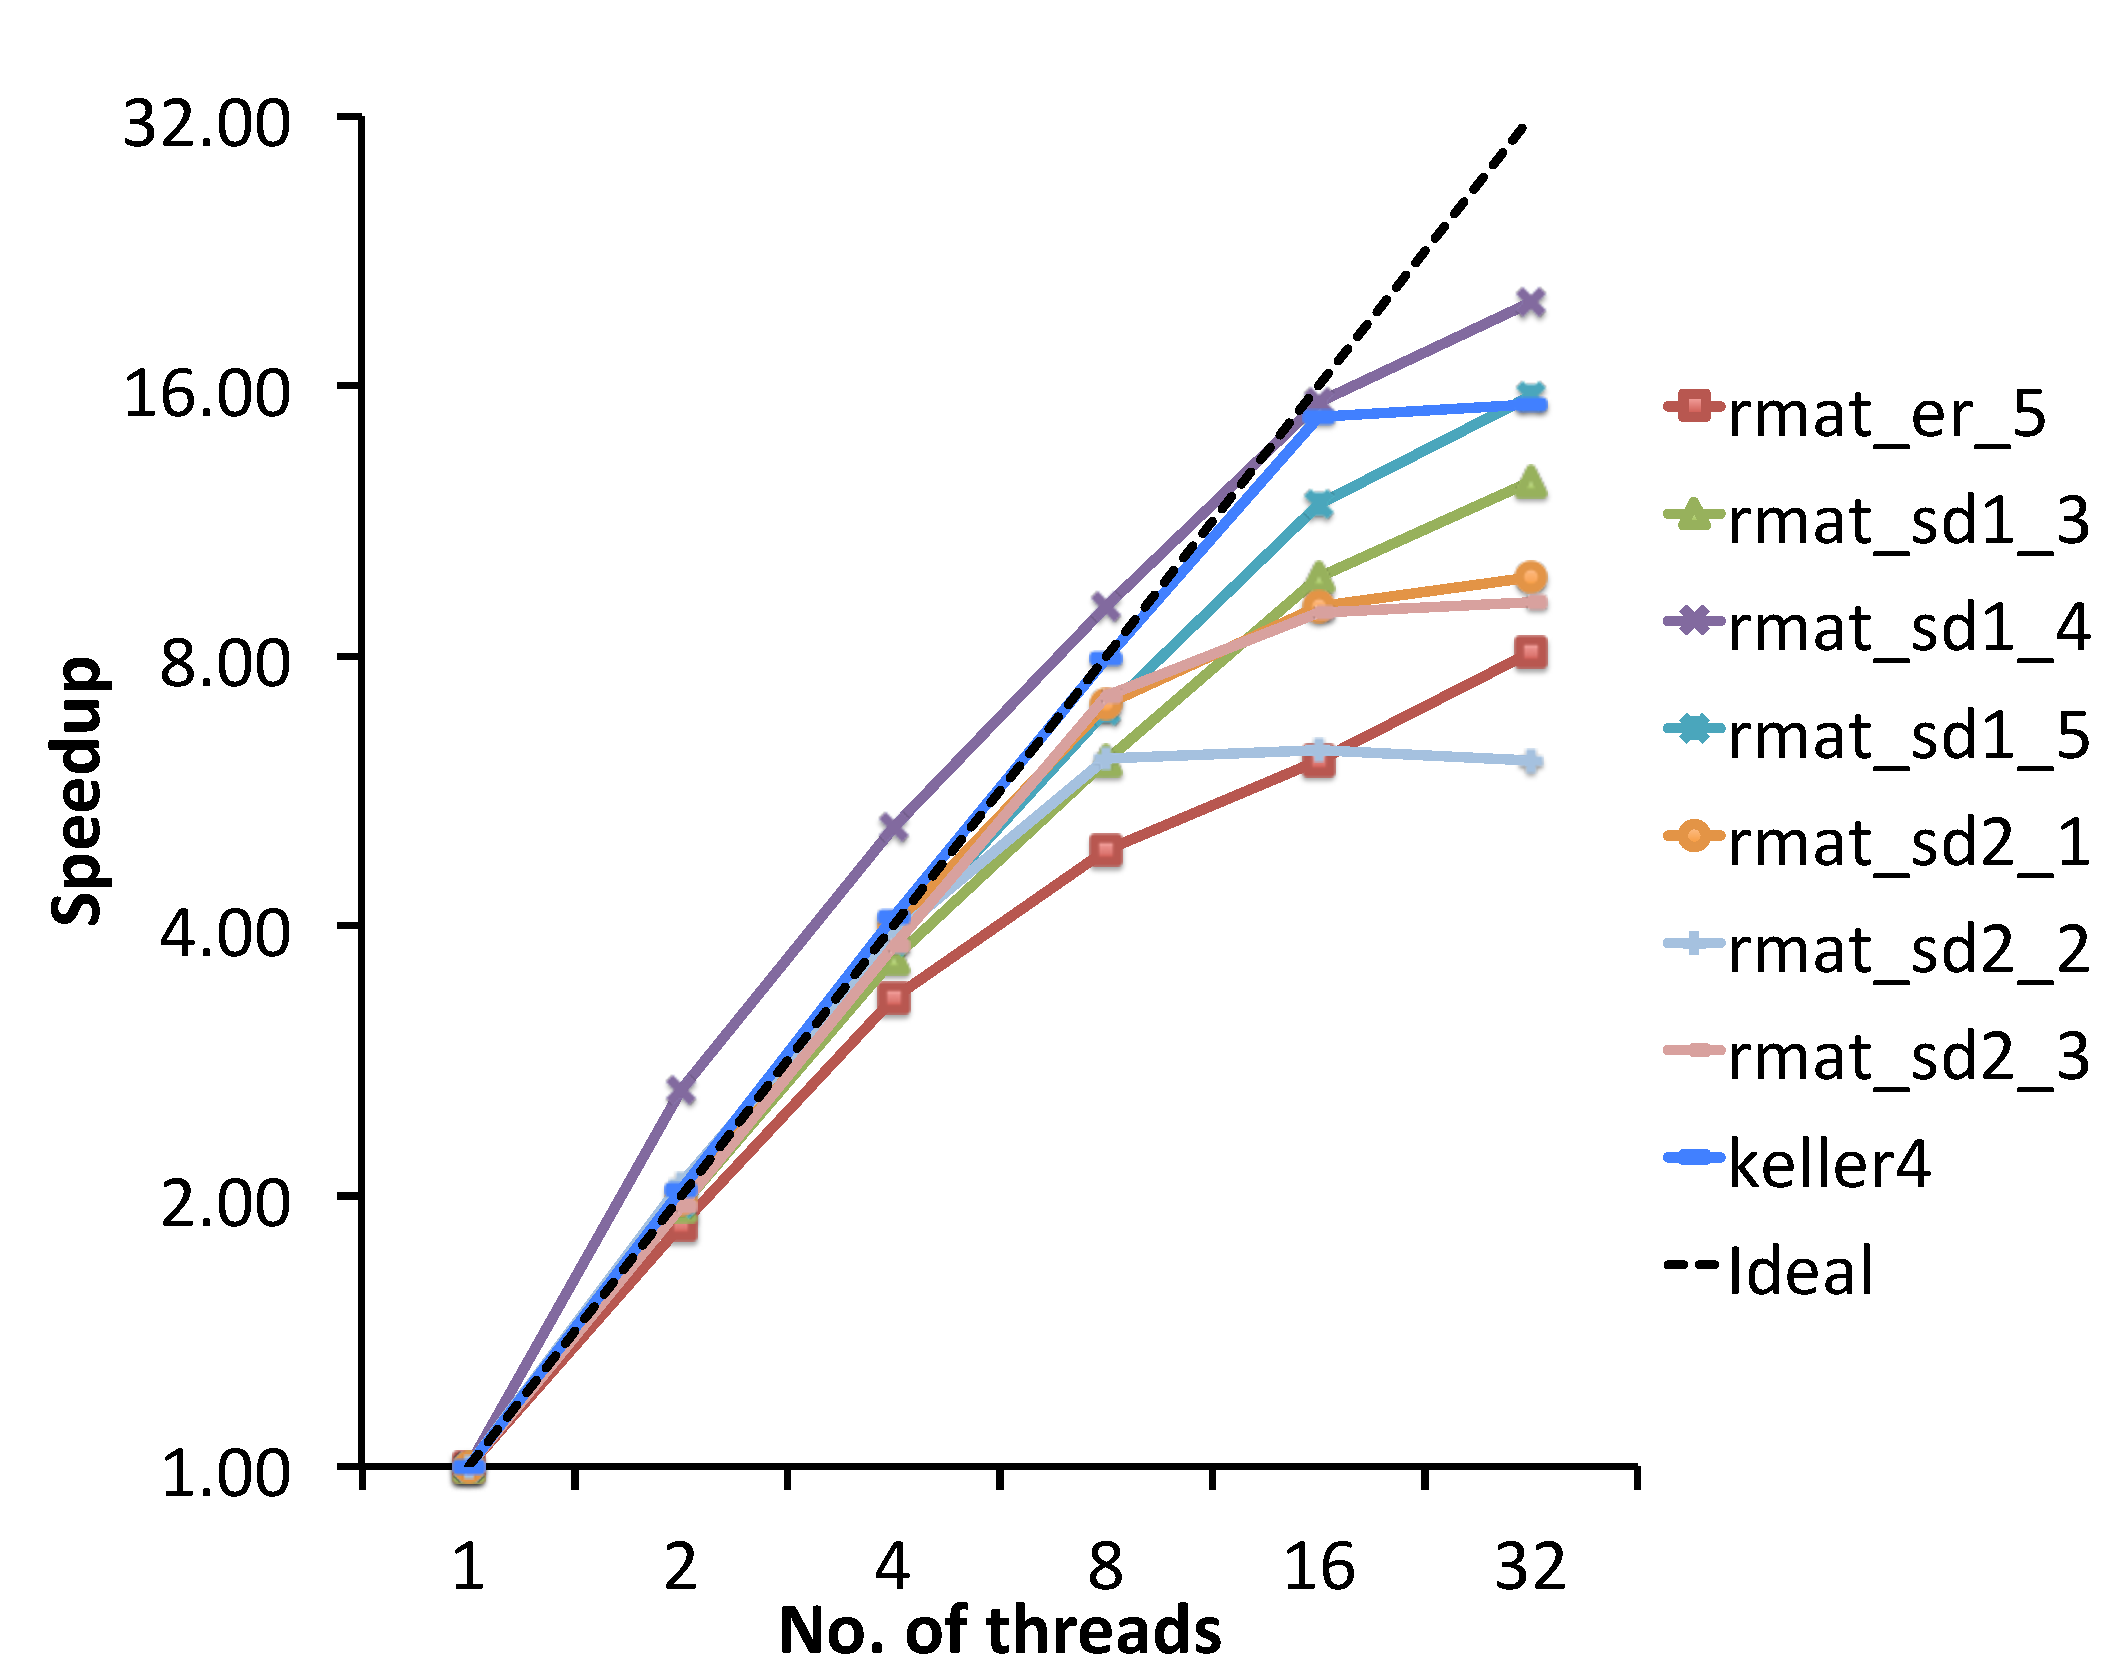
\includegraphics[scale=0.17]{parallel_other_speedup.pdf}
    
%%\vspace{-30pt}
 \caption{Performance (timing and speedup plots) of shared-memory parallelization on graphs in the test-bed. Graphs whose sequential runtime is less than 5 seconds are omitted. The top set of figures show performance on the real-world graphs, whereas the bottom set show results for the RMAT graphs.}
\label{fig-parallel_perf}
\end{figure}


Figure \ref{fig-parallel_perf} shows the timings and speedups we obtained for the real-world and RMAT graphs separately. We omitted graphs whose sequential runtimes were less than 5 seconds as they were too low to measure and do meaningful assessment of parallelization performance. For most of the real-world graphs, one can see from the figure that we obtained near-linear scaling of runtimes and speedups when up to 16 threads are used. The only exception is the graph 
{\emph as-Skitter}. The relatively poorer scaling there is likely due to the fact that the instance has a relatively large maximum clique, and hence the core (thread) which computes it spends relatively large amount of time computing it while other cores (threads) which have completed their processing of the remaining vertices remain idle. 
For the other instances of the real-world graphs, the maximum speedup we obtained 
while using 32 cores/threads is around 22$\times$. 

For the RMAT graphs, it can seen that the scaling of the runtime and speedups vary with the structures (RMAT parameters) of the instances. We observed super-linear speedups for a couple of the instances. For the others, the algorithm scales fairly well up to 8 threads, and begins to
degrade thereafter. The speedups we obtained range between 6$\times$  to 20$\times$ when 32 threads are used.





%The effects of pruning could, although, be tolerably compromised in order to enable the parallel computation by allowing the processors to use the locally computed maximum clique value as the lower bound for pruning until regular synchronization steps, during which it is updated to the global value of the maximum clique across all processors.

%When done in parallel, the for loop in Algorithm \ref{alg:mClq} can be distributed among different $p$ computational units which can compute different values for $max$ in parallel. In the next step, a reduce operation can be used to find the maximum of the $p$ values.

%In this section we show the results of parallelization of our exact algorithm on shared memory architectures. In our algorithm, there is no dependency or strict order in which the vertices have to be computed unlike other previous algorithms. The sizes of the largest cliques containing different vertices can be computed mostly independently, and thus can be done in parallel by different computational units.


%\begin{figure}
%        \centering
%        \begin{subfigure}[b]{0.5\textwidth}
%                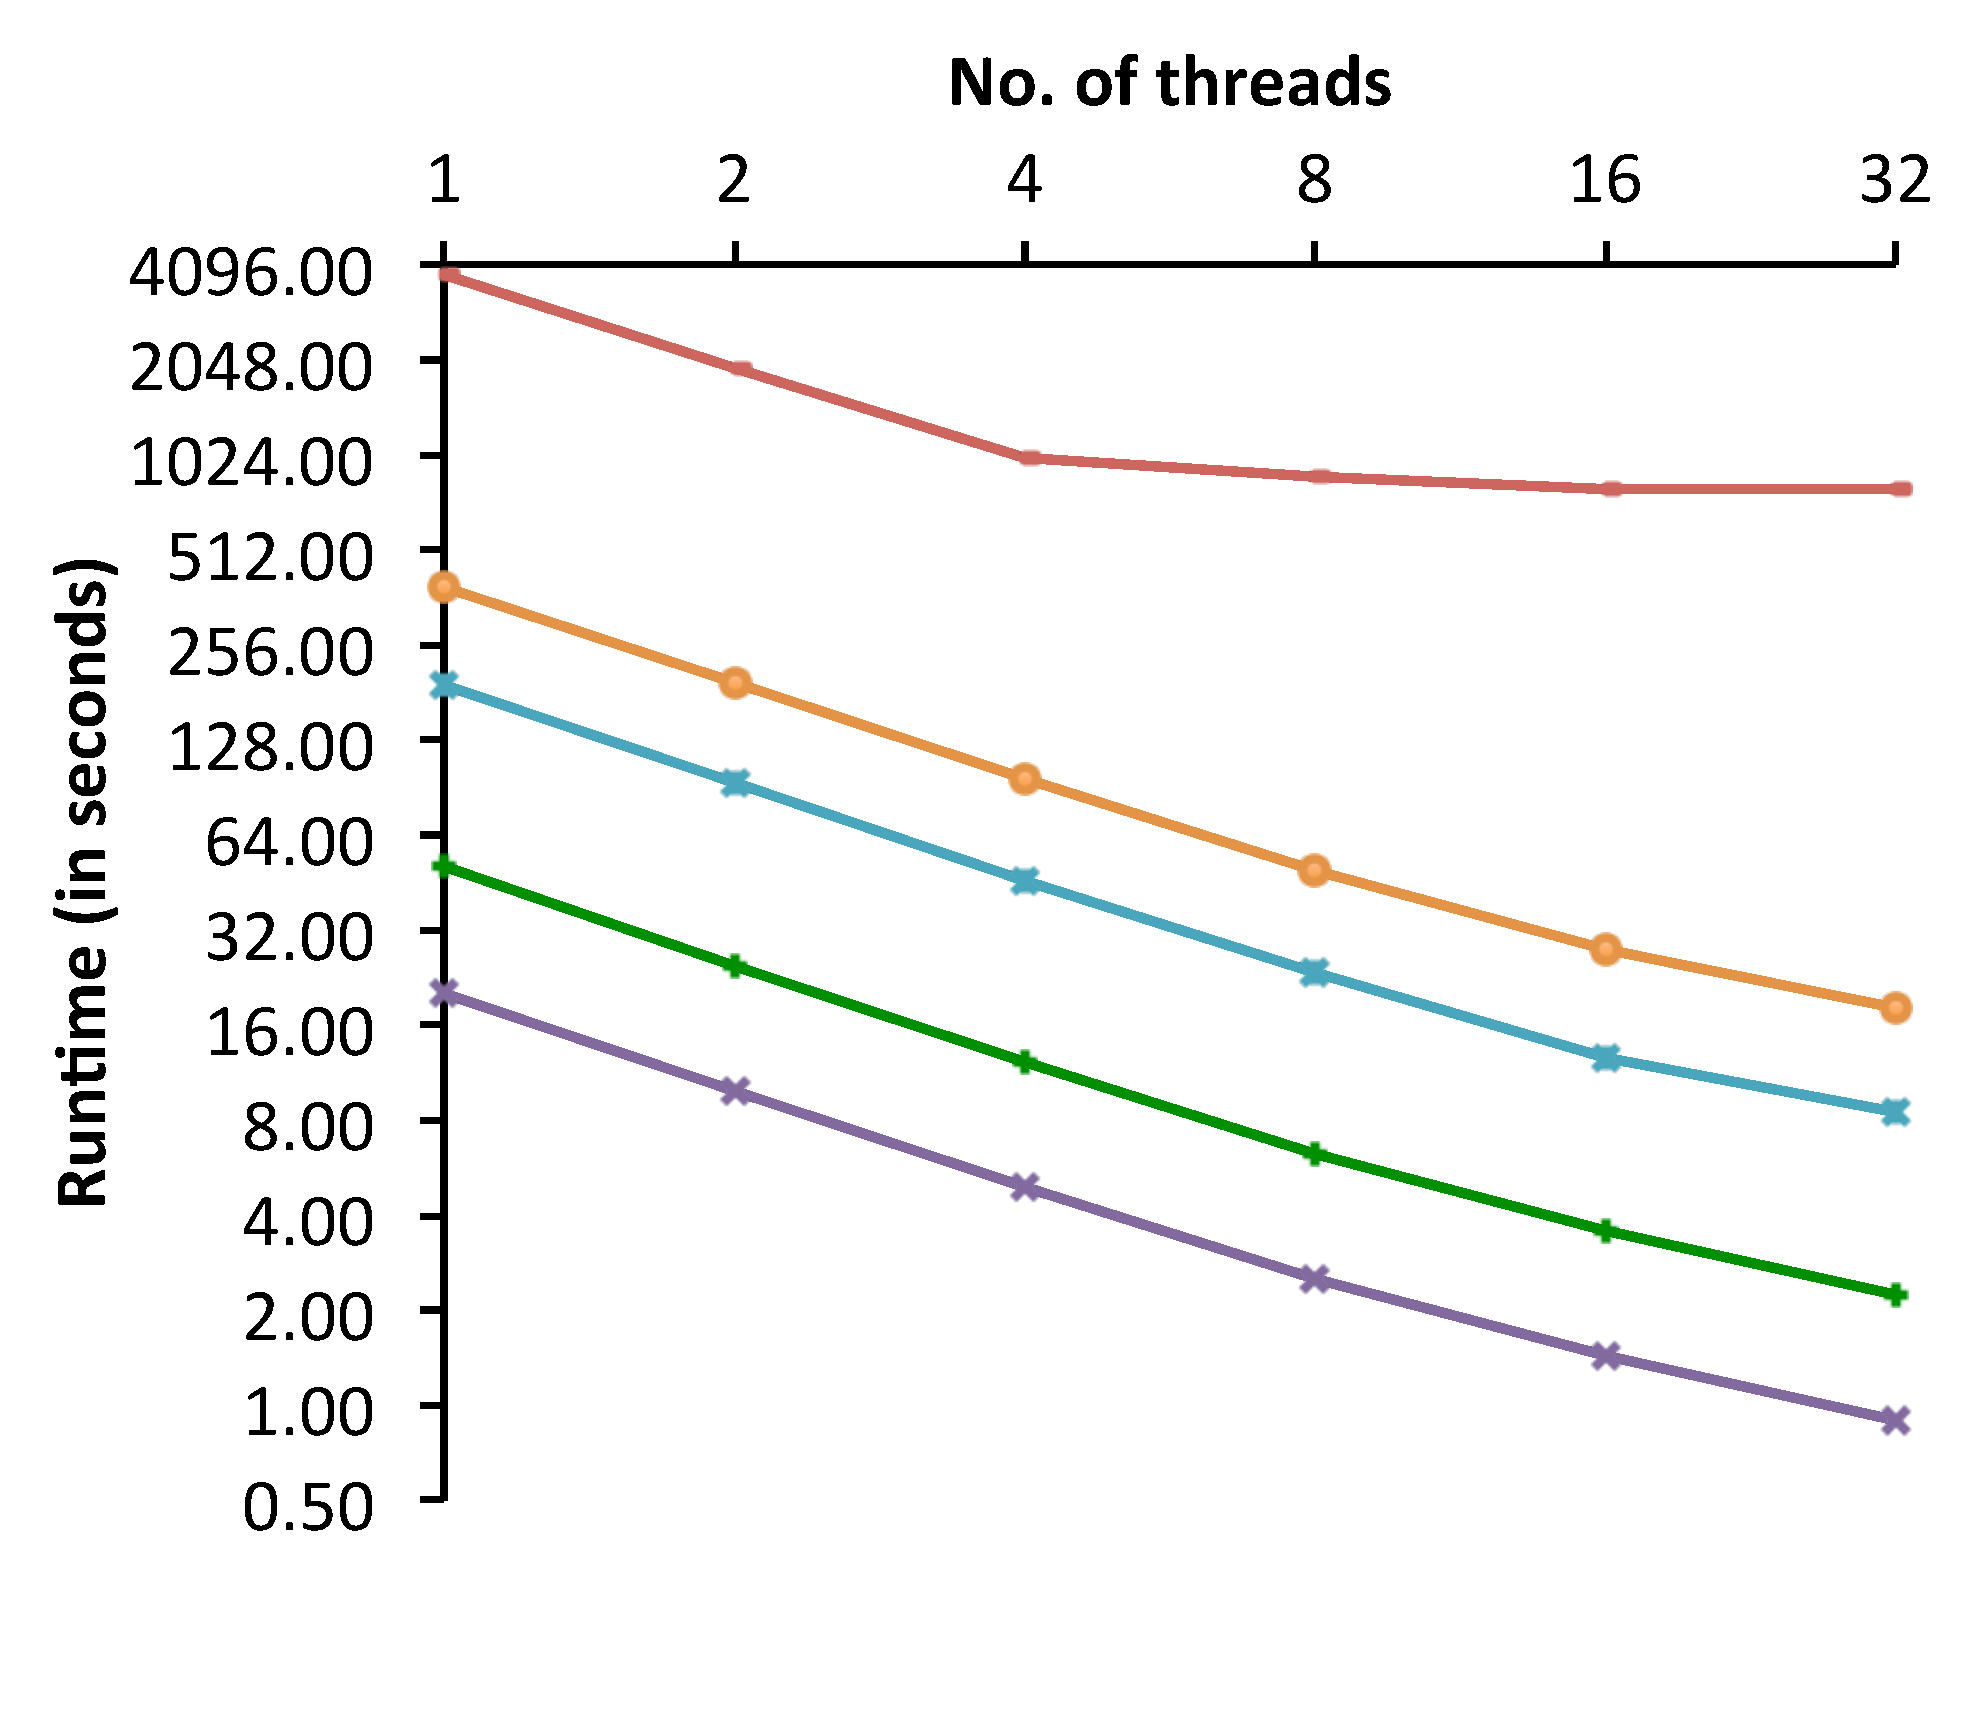
\includegraphics[width=\textwidth]{parallel_realworld_timing.pdf}
%                \caption{Timing results}
%                \label{fig:timing_realworld}
%        \end{subfigure}%
%        ~ %add desired spacing between images, e. g. ~, \quad, \qquad etc.
%          %(or a blank line to force the subfigure onto a new line)
%        \begin{subfigure}[b]{0.5\textwidth}
%                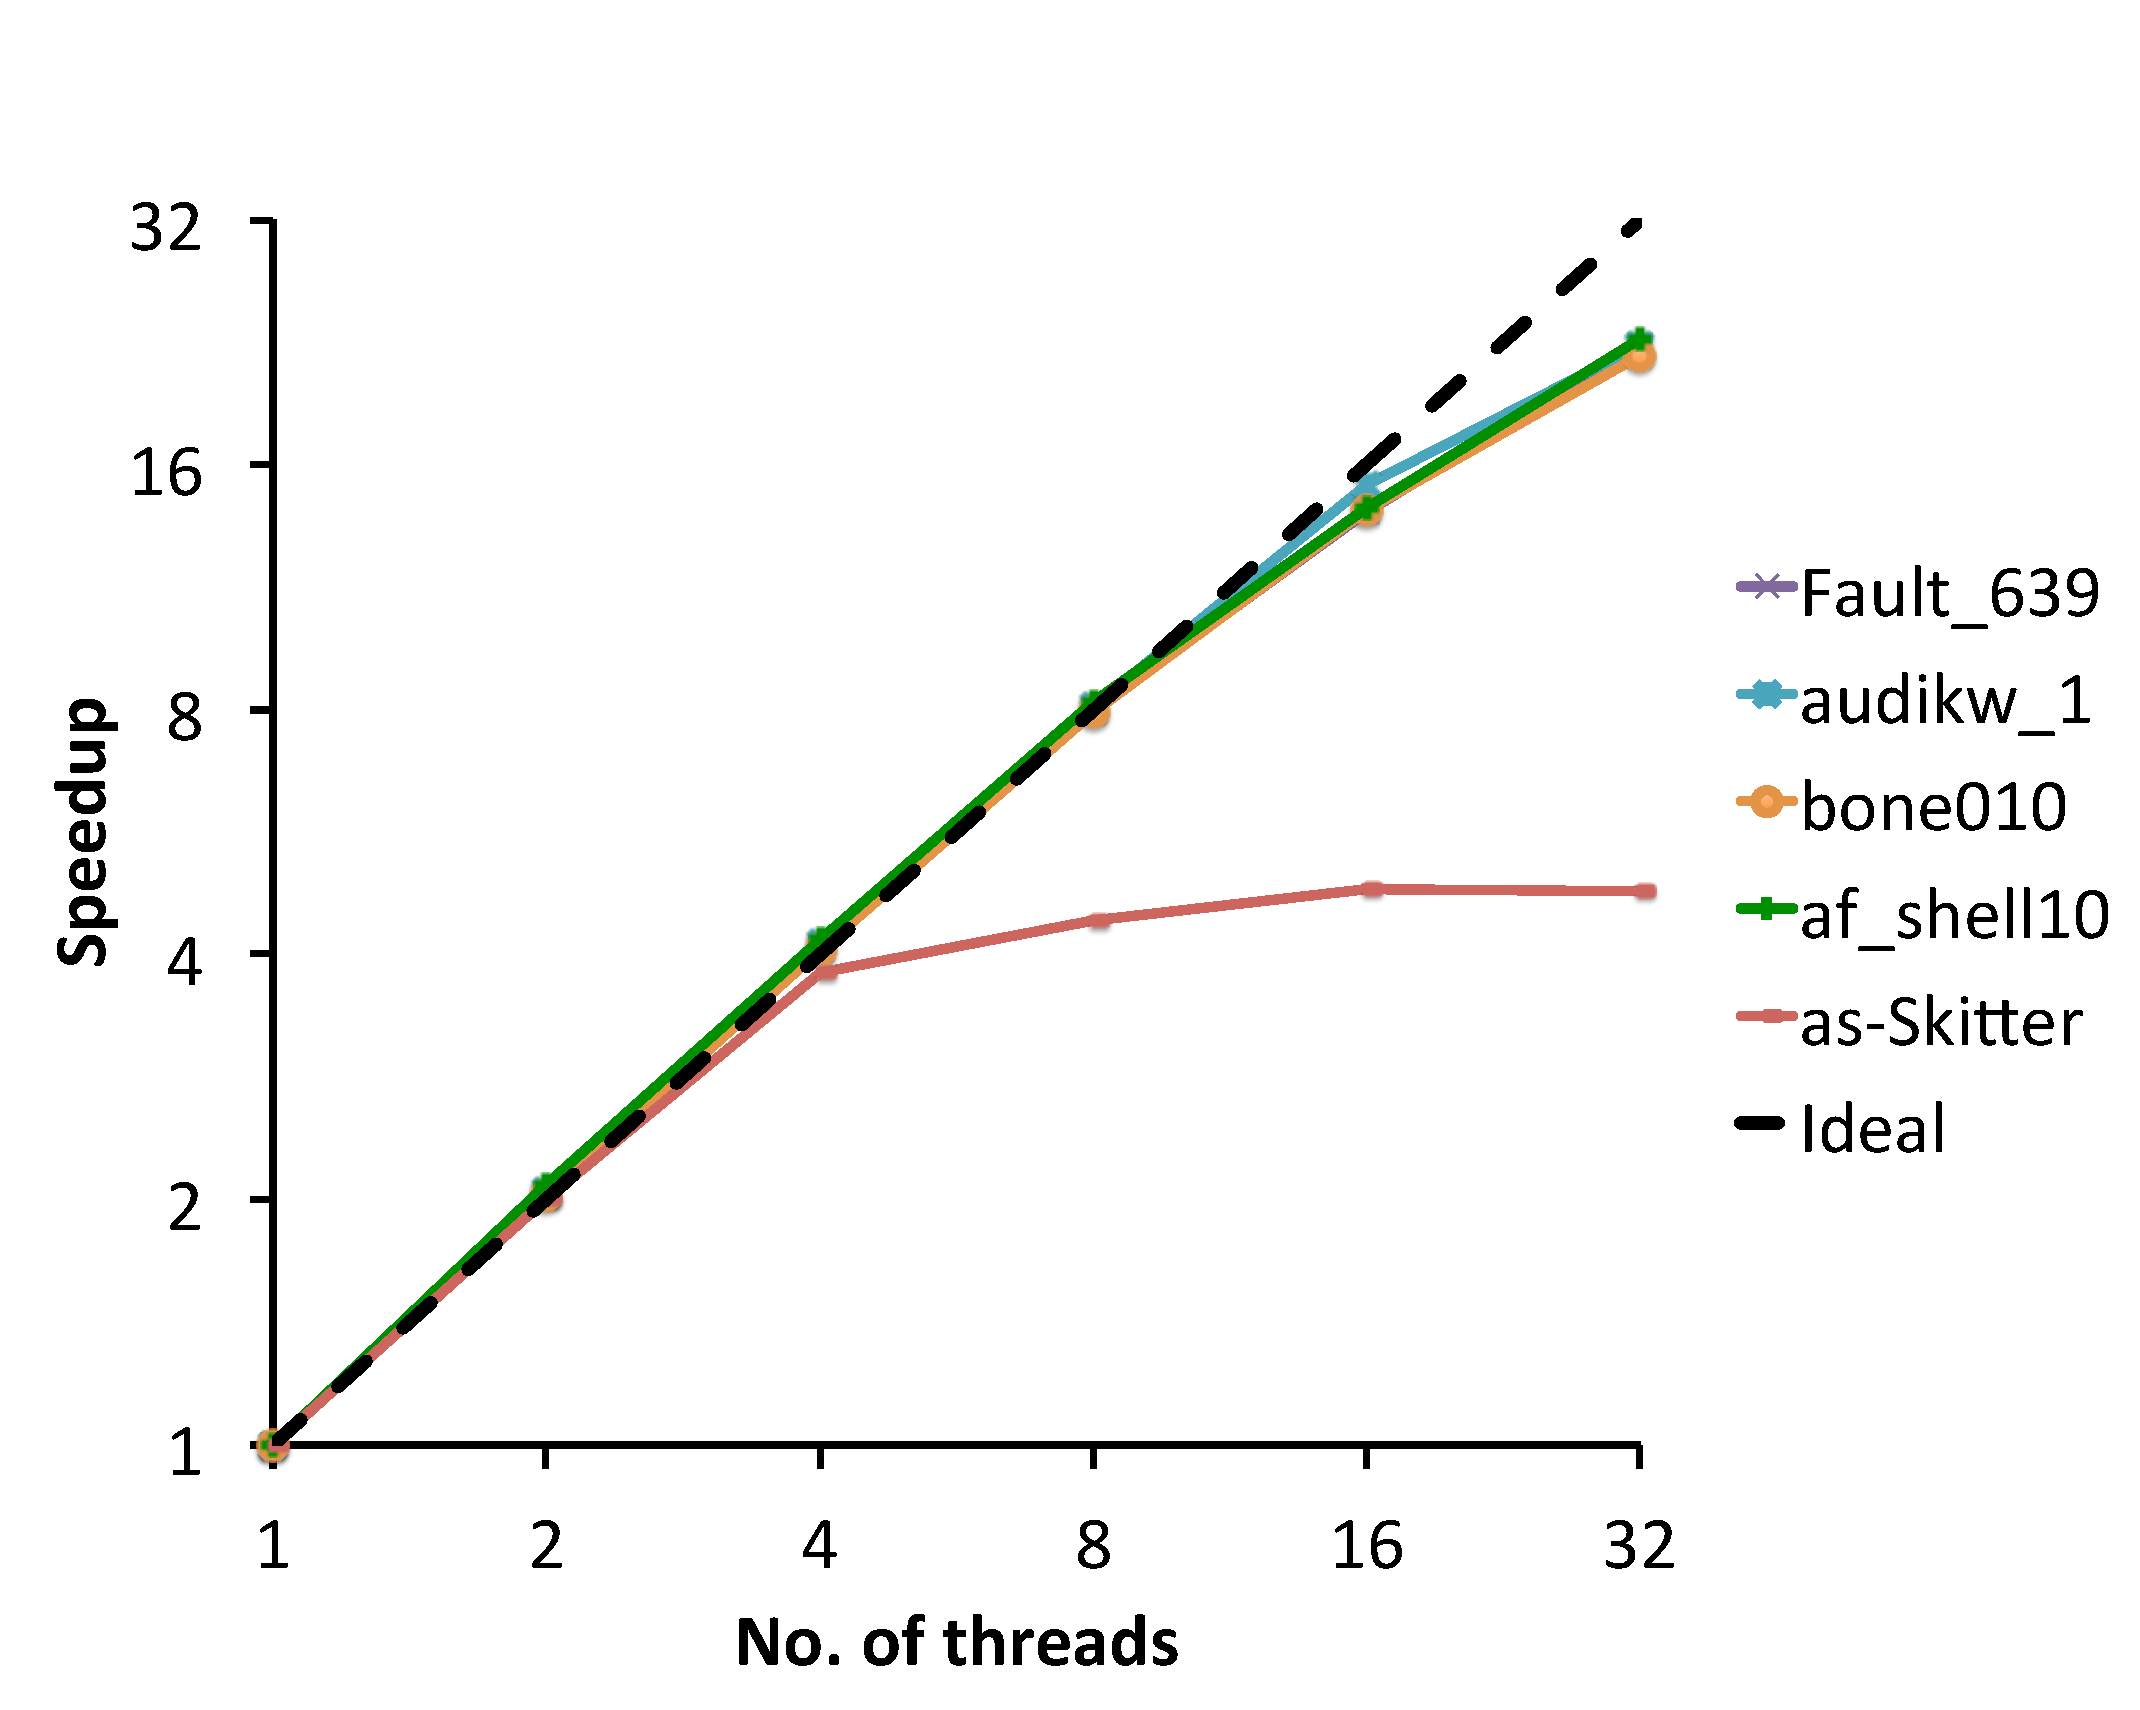
\includegraphics[width=\textwidth]{parallel_realworld_speedup.pdf}
%                \caption{Speedup results}
%                \label{fig:speedup_realworld}
%        \end{subfigure}
%        \caption{Performance of shared-memory parallelization on real-world graphs}\label{fig:animals}
%\end{figure}
%
%
%\begin{figure}
%        \centering
%        \begin{subfigure}[b]{0.5\textwidth}
%                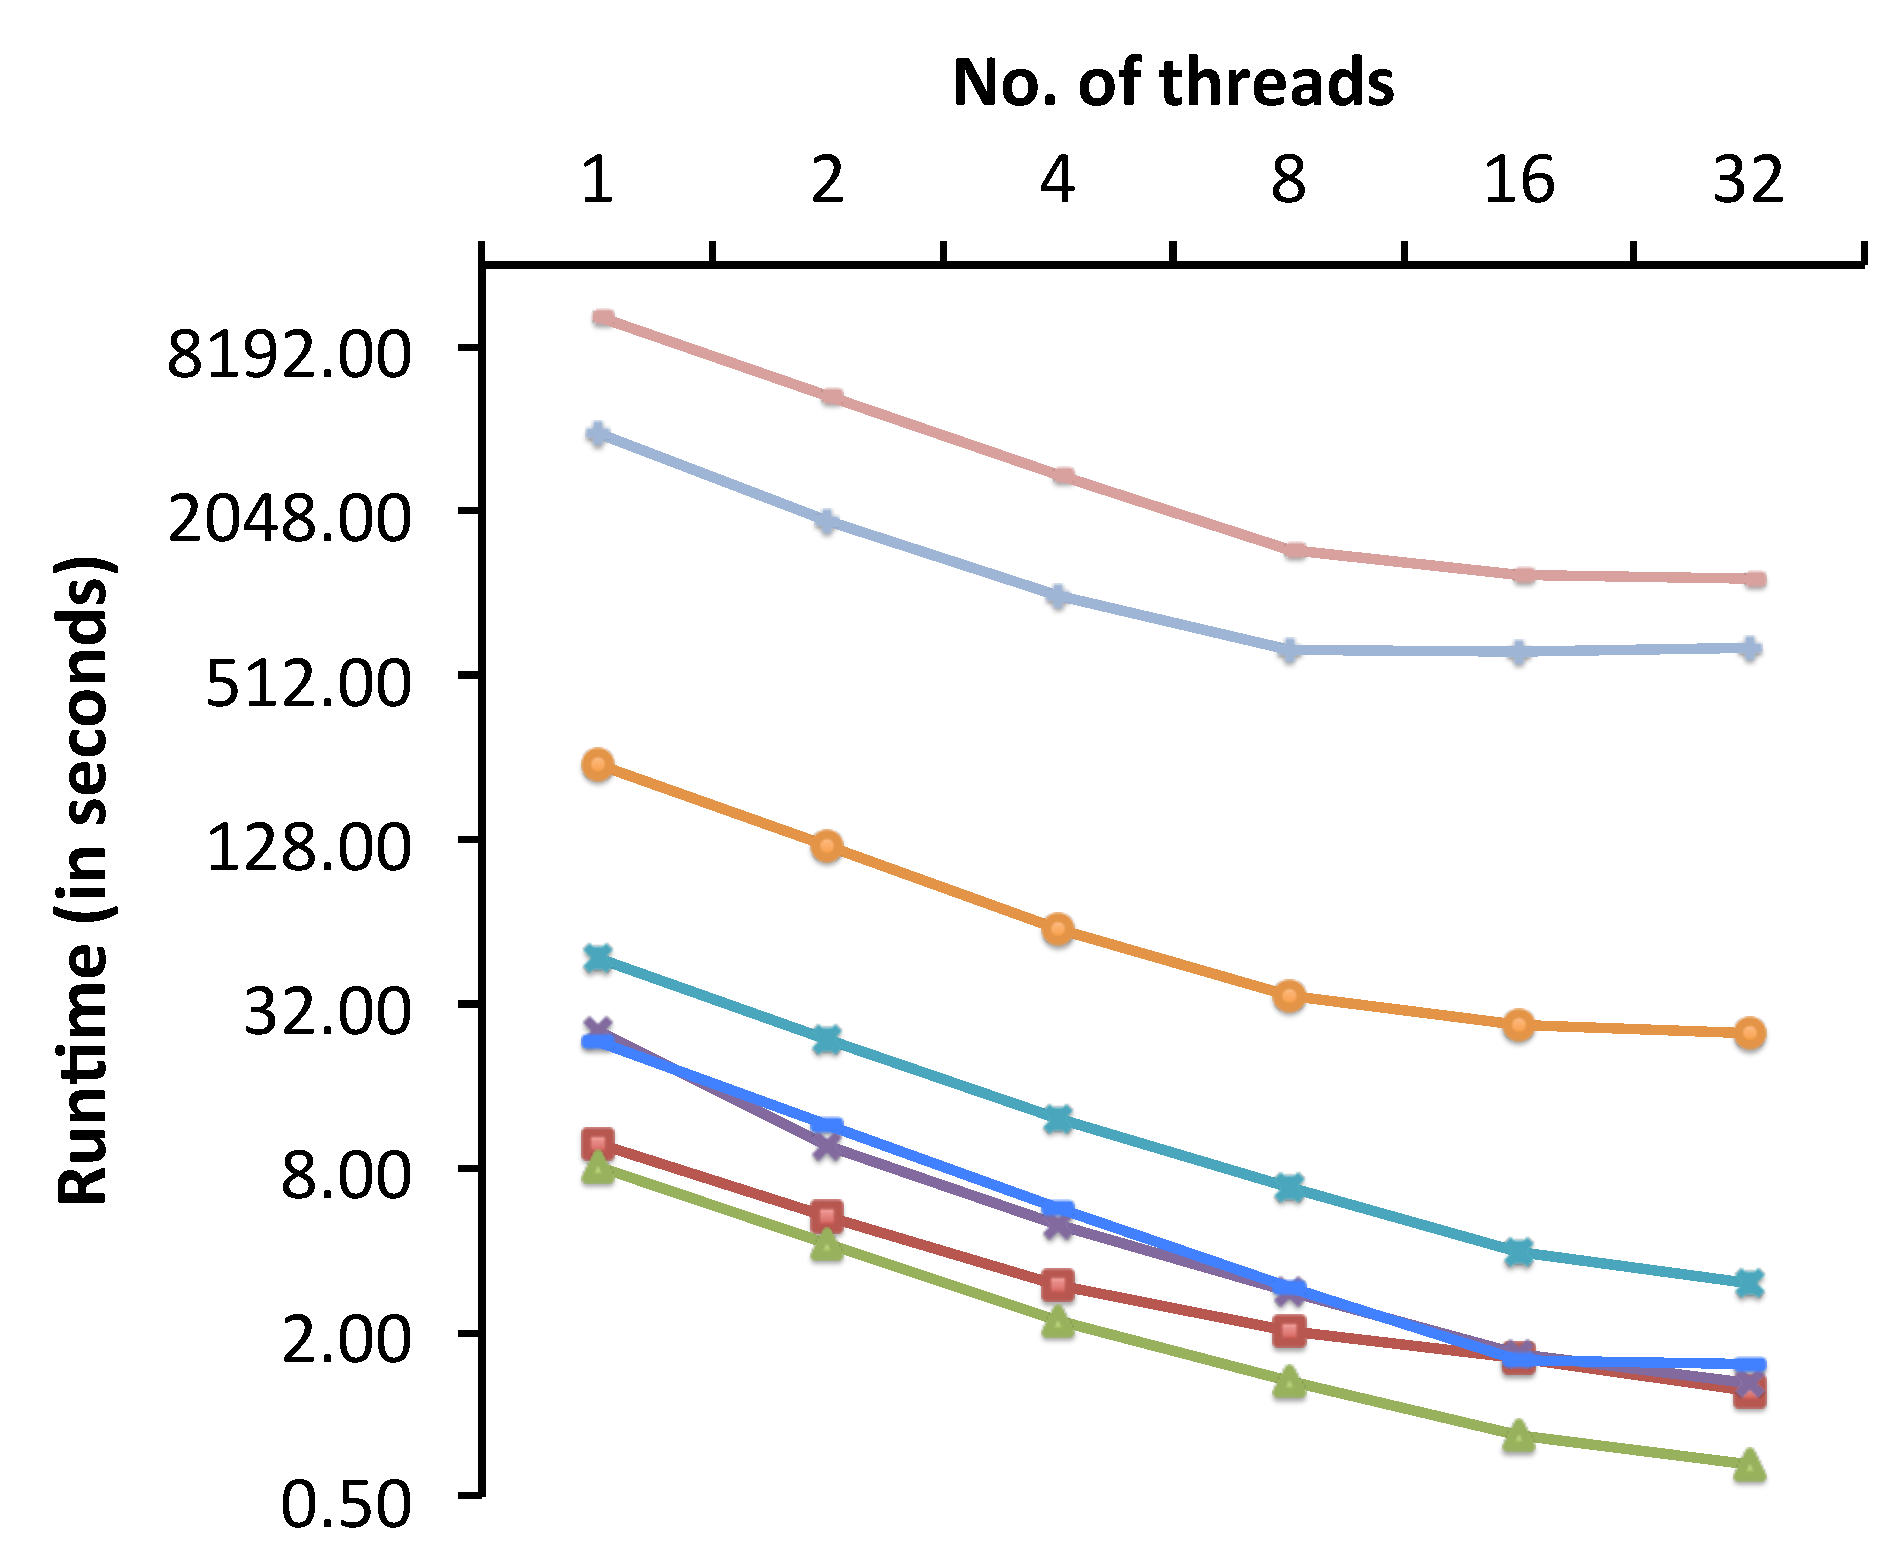
\includegraphics[width=\textwidth]{parallel_other_timing.pdf}
%                \caption{Timing results}
%                \label{fig:timing_realworld}
%        \end{subfigure}%
%        ~ %add desired spacing between images, e. g. ~, \quad, \qquad etc.
%          %(or a blank line to force the subfigure onto a new line)
%        \begin{subfigure}[b]{0.5\textwidth}
%                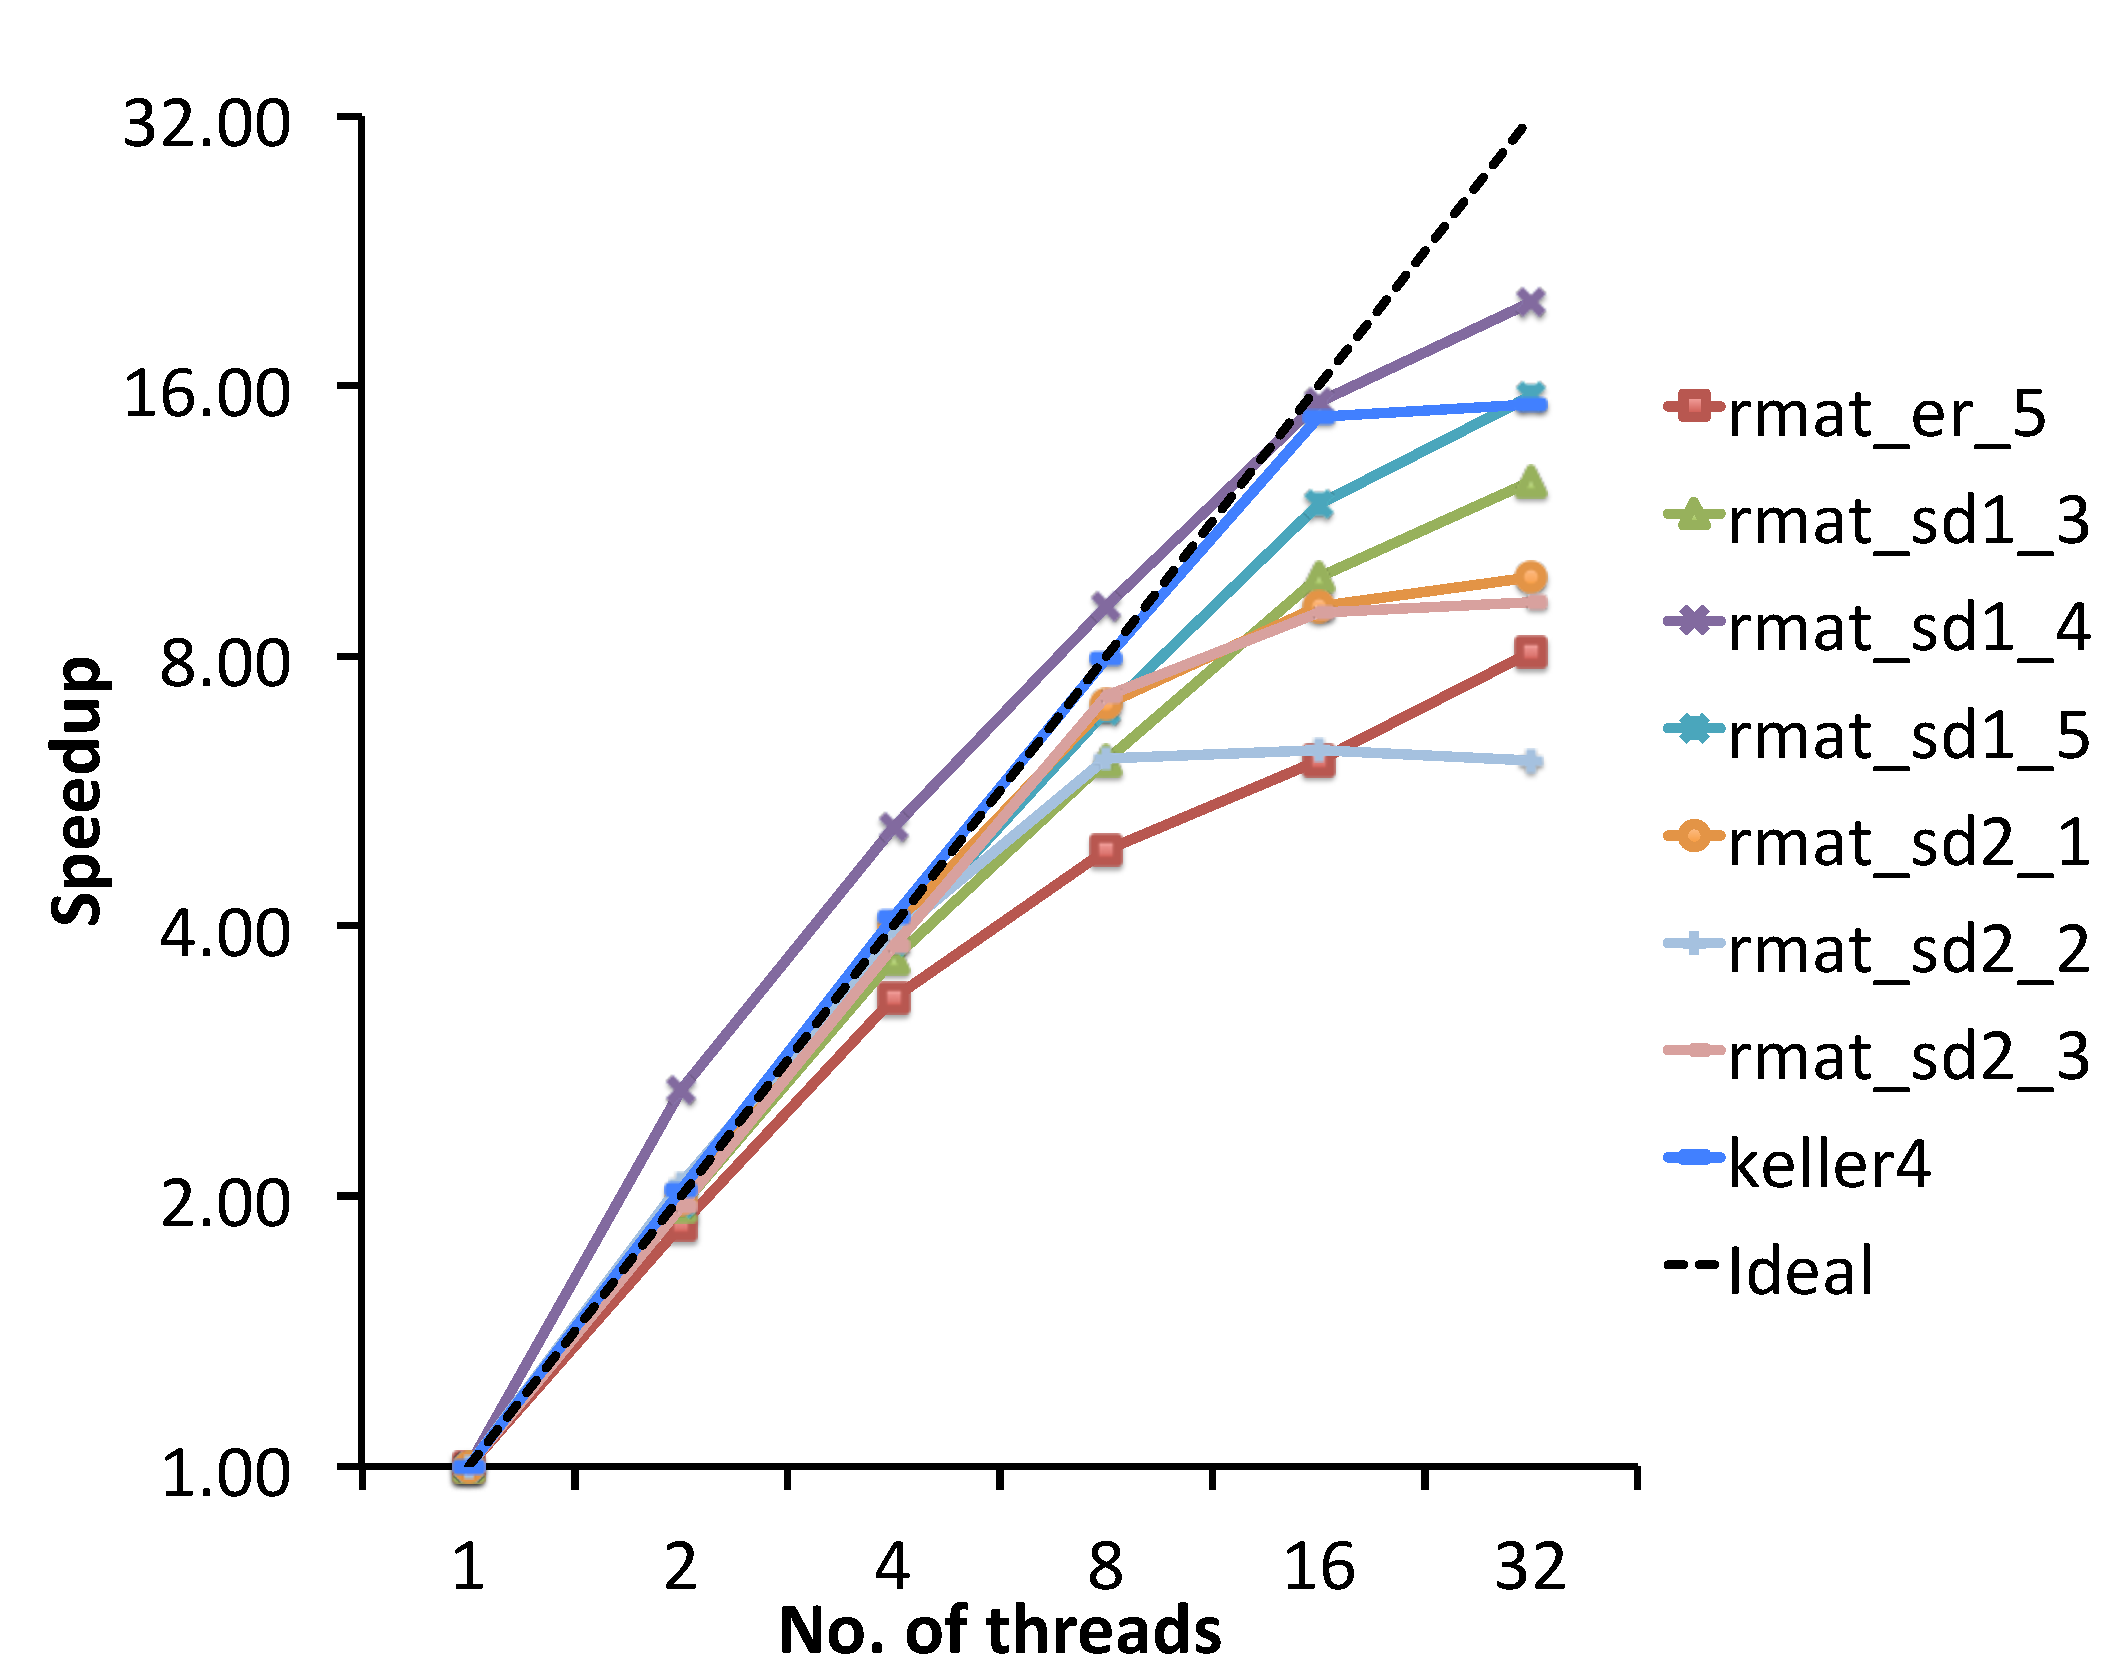
\includegraphics[width=\textwidth]{parallel_other_speedup.pdf}
%                \caption{Speedup results}
%                \label{fig:speedup_realworld}
%        \end{subfigure}
%        \caption{Performance of shared-memory parallelization on real-world graphs}\label{fig:parallel_perf}
%\end{figure}
%







\subsection{Example of an application in social network analysis}
\label{sec:applications}

We conclude this section on experiments with a small example 
demonstrating the application of the clique algorithms for detecting overlapping communities in social networks. 
In many real networks vertices may belong to more than one group, and such groups form overlapping communities. Classical examples are social networks, where an individual usually belongs to different circles at the same time, from that of work colleagues to family, sport associations, etc. 
Finding overlapping communities is a challenging problem \cite{Fortunato_2010}.
Clique algorithms are one way in which a solution can be found.  
%A detailed overview of community detection methods, and the significance and complexity involved in overlapping community findingcan be found in \cite{Fortunato_2010}.

%\vspace{-20pt}
\begin{figure}%[h!]
  \centering
    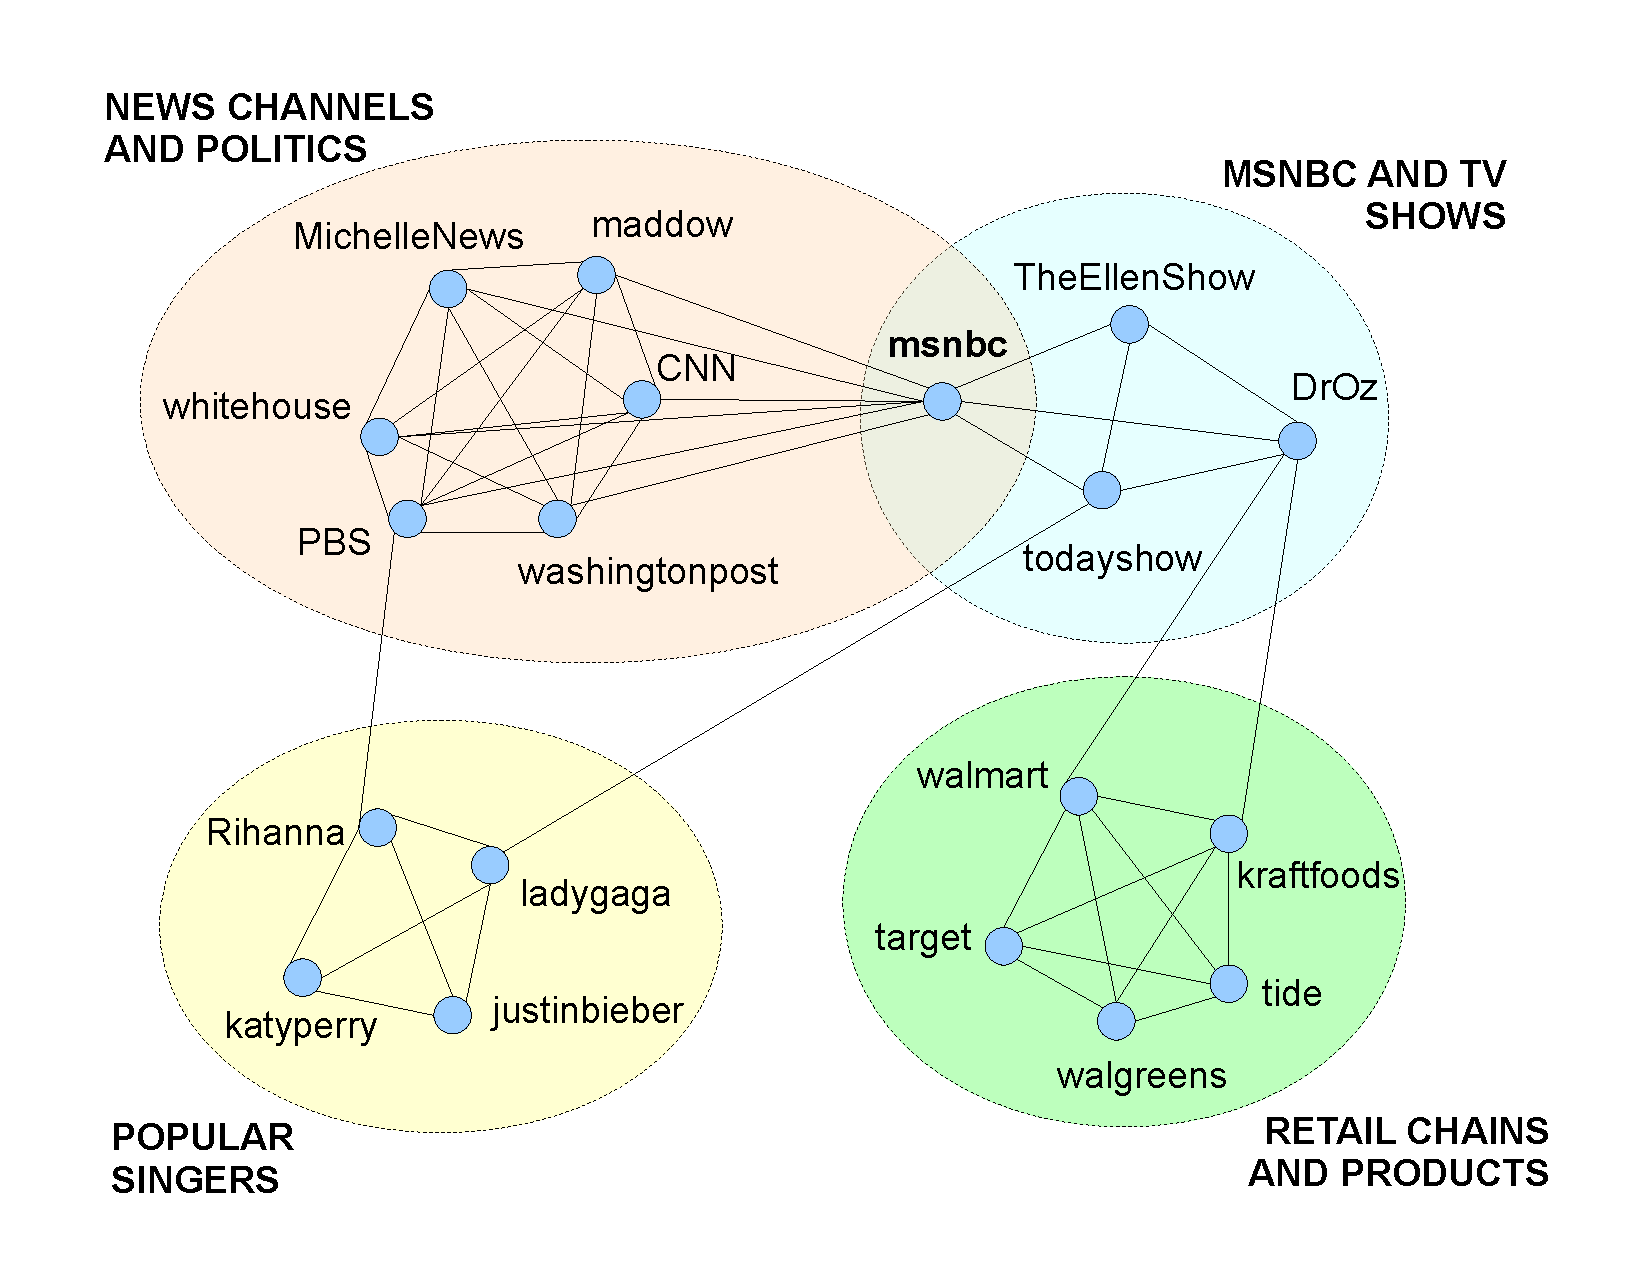
\includegraphics[width=1\textwidth]{communities.pdf}
%\vspace{-30pt}
  \caption{Some Facebook communities detected by our max clique heuristic.}
\label{fig-communities}
\end{figure}
%\vspace{-10pt}

%\footnotetext{http://www.facebook.com}
For our small experiment, we use data collected from Facebook\footnote[1]{http://www.facebook.com}.
Every user on Facebook has a {\it wall}, which is a the user's profile space that allows the posting of messages, often short or temporal notes by other users. The user comments and user information from specific {\it walls} are publicly available and we collected them using Facebook API. We constructed a graph with the {\it walls} as vertices. Any two users who have commented on the same {\it wall} indicate a connection between the {\it walls}, and we form an edge between them. There could be many common users for each wall, and so we assigned edge weights by Jacard index or similarity coefficient \cite{Leydesdorff}. Once this is done for all {\it walls}, we retained only those edges which have weights above a chosen threshold, indicating a strong correlation. The threshold is a user's choice and decides both the size and the number of communities found.
% If an edge already exists, we increase the edge weight by 1. Once this is done for all {\it walls}, the edge weights are normalized, and we retain only those edges which have edge weights above a chosen threshold (we use 0.01), indicating a strong correlation.

%duplicate removal
We modified our heuristic to retain the largest maximum clique containing each node. 
%This is done by simply substituting Lines 3 and 4 of Algorithm \ref{alg:clqHeu}, with a simple routine that stores each clique in a preferred data structure. 
The exact algorithm could have also been used instead of the heuristic for this purpose. We choose the heuristic since it is much faster and for this particular problem of community detection the accuracy of the size of cliques formed is not critical.

Figure \ref{fig-communities} shows some of the cliques/communities detected. We see two isolated communities, one for popular singers, and another for retail chains and products. We also see a community for news channels and politics, and a community of MSNBC and popular TV shows. The highlight of this experiment  is that the
clique algorithm allows a node to be a member of more than one community giving an overlapping community structure. Although the {\it news channels and politics} and {\it MSNBC and tv shows} communities are not directly related and have different members, they share a common member.
%add from nature paper why this is significant. coexistence of their structural subunits 



%\vspace{-6pt}
\section{Conclusion}
\label{sec:conclusion}
%\vspace{-10pt}

We presented a new exact and a new heuristic algorithm for the maximum clique problem.
We performed extensive experiments on three broad categories of graphs comparing the 
performance of our algorithms to the algorithms due to
Carraghan and Pardalos (CP) \cite{pardalos},
\"{O}sterg\.{a}rd ({\it cliquer}) \cite{ostergard} and
Konc and Jane\v{z}i\v{c} ({\it MCQD+CS}) \cite{konc2007improved}.
For DIMACS benchmark graphs and certain dense synthetic graphs ({\it rmat\_sd2}), our new exact algorithm performs comparably with the CP algorithm, but slower than {\it cliquer}
and {\it MCQD+CS}. 
For large sparse graphs, both synthetic and real-world, our new algorithm runs
several orders of magnitude faster than the other three. 
And its general runtime is observed to grow nearly linearly with the size of the graphs. 
The heuristic, which runs orders of magnitude faster than our exact algorithm and the others, gave optimal solution for 83\% of the test cases, and when it is sub-optimal, its accuracy ranged between 0.83 and 0.99.
We also showed how the algorithms can be parallelized. Finally, we illustrated a simple application of the algorithms in the design of methods for detecting overlapping communities in networks. 

Maximum clique detection is often avoided by practitioners from being used as a component in 
a network analysis algorithm on the grounds of its NP-hardness. The results shown here suggest that they need
not be as maximum cliques can in fact be detected rather quickly for most real-world networks that are characterized by sparsity and other structures well suited for branch-and-bound type algorithms.

Our comparison with existing algorithms is understandably not exhaustive.
We have compared against a reasonable sample representatives with emphasis on those
that have publicly available implementations. There are a number of algorithms that do not have publicly available implementation (e.g. \cite{walcom,AAAI101611}) and that would be interesting to compare against in future work. 
%Further, the MCQD implementation uses an adjacency matrix, whereas our algorithm uses an adjacency list to represent the graph. Although it is unlikely for the overall results to be drastically different with a change in the graph representation, it will be interesting to study to what degree the performance will change with
%the change in graph representation.
%The exact algorithm was in general  found to be less successful on relatively dense graphs.
%An interesting line of investigation would be to study ways to overcome this.
%The heuristic's performance is impressive as presented; still it is worthwhile
%to compare with other existing heuristics approaches such as \cite{heu1,heu2}. 
%Another line for future work would be to characterize the class(es) of graphs for which the heuristic is expected to return near-optimal solution.

%\vspace{-6pt}
\section*{Acknowledgements}
%\vspace{-6pt}
%This work is supported in part by NSF award numbers CCF-0621443, OCI-0724599, CCF-0833131, CNS-0830927, IIS-0905205, OCI-0956311, CCF-0938000, CCF-1043085, CCF-1029166, and OCI-1144061, and in part by DOE grants DE-FG02-08ER25848, DE-SC0001283, DE-SC0005309, DE-SC0005340, and DE-SC0007456. 
This work is supported in part by the following grants: NSF awards CCF-0833131, CNS-0830927, IIS-0905205, CCF-0938000, CCF-1029166, and OCI-1144061; DOE awards DE-FG02-08ER25848, DE-SC0001283, DE-SC0005309, DESC0005340, and DESC0007456; AFOSR award FA9550-12-1-0458. 
The work of Assefaw Gebremedhin is supported by the NSF
award CCF-1218916 and by the DOE award DE-SC0010205.

%\vspace{-2pt}
%\bibliographystyle{gOMS}
%\vspace{-4pt}
%\bibliography{ref}

%\vspace{-6pt}
\begin{thebibliography}{10}
\providecommand{\url}[1]{\texttt{#1}}
\providecommand{\urlprefix}{URL }
%\vspace{-10pt}

\bibitem{heu1}
{D.~Andrade, M.~Resende, and R.~Werneck}, {\em Fast local search for the
  maximum independent set problem}, Journal of Heuristics, 18 (2012),
  pp.~525--547.

\bibitem{Augustson:1970:AGT:321607.321608}
J.G. Augustson and J. Minker, \emph{An analysis of some graph theoretical
  cluster techniques}, J. ACM 17 (1970), pp. 571--588.

\bibitem{babel1990branch}
L. Babel and G. Tinhofer, \emph{A branch and bound algorithm for the maximum
  clique problem}, Mathematical Methods of Operations Research 34 (1990), pp.
  207--217.

\bibitem{pajek2006}
V. Batagelj and A. Mrvar, \emph{Pajek datasets}  (2006),
  \urlprefix\url{http://vlado.fmf.uni-lj.si/pub/networks/data/}.

\bibitem{RePEc:eee:csdana:v:48:y:2005:i:2:p:431-443}
V. Boginski, S. Butenko, and P.M. Pardalos, \emph{Statistical analysis of
  financial networks}, Computational Statistics \& Data Analysis 48 (2005), pp.
  431--443.

\bibitem{Bomze99themaximum}
I.M. Bomze, M. Budinich, P.M. Pardalos, and M. Pelillo, \emph{The Maximum
  Clique Problem}, in \emph{Handbook of Combinatorial Optimization}, Kluwer
  Academic Publishers, 1999, pp. 1--74.

\bibitem{Bonner:1964:CT:1662386.1662389}
R.E. Bonner, \emph{On some clustering techniques}, IBM J. Res. Dev. 8 (1964),
  pp. 22--32.

\bibitem{brouwer}
A.E. Brouwer, J.B. Shearer, N.J.A. Sloane, and W.D. Smith, \emph{A new table of
  constant weight codes.}, IEEE Transactions on Information Theory  (1990), pp.
  1334--1380.

\bibitem{pardalos}
R. Carraghan and P. Pardalos, \emph{An exact algorithm for the maximum clique
  problem}, Oper. Res. Lett. 9 (1990), pp. 375--382.

\bibitem{Chakrabarti:2006:GML:1132952.1132954}
D. Chakrabarti and C. Faloutsos, \emph{Graph mining: Laws, generators, and
  algorithms}, ACM Comput. Surv. 38 (2006).

\bibitem{Davis97theuniversity}
T.A. Davis and Y. Hu, \emph{The university of florida sparse matrix
  collection}, ACM Transactions on Mathematical Software (TOMS) 38 (2011), pp.
  1:1--1:25.

\bibitem{Domingos:2001:MNV:502512.502525}
P. Domingos and M. Richardson, \emph{Mining the network value of customers}, in
  \emph{Proc. of the 7th ACM SIGKDD KDD'01}, KDD '01, San Francisco,
  California, ACM, New York, NY, USA, 2001, pp. 57--66.

\bibitem{Doreian1994267}
P. Doreian and K.L. Woodard., \emph{Defining and locating cores and boundaries of social networks}, {\em Social Networks}, 16(4):267 -- 293, 1994.

%\bibitem{Edachery99graphclustering}
%J. Edachery, A. Sen, F.J. Brandenburg, F.J. Br, and L.F. Informatik,
%  \emph{Graph Clustering Using Distance-k Cliques}, in \emph{Proc. of Graph
%  Drawing}, Springer-Verlag, 1999, pp. 98--106.

\bibitem{Faloutsos:1999:PRI:316188.316229}
M. Faloutsos, P. Faloutsos, and C. Faloutsos, \emph{On power-law relationships
  of the Internet topology}, in \emph{Proc. of the conference on Applications,
  technologies, architectures, and protocols for computer communication},
  SIGCOMM '99, Cambridge, Massachusetts, United States, ACM, 1999, pp.
  251--262.

\bibitem{Ferronato20083922}
M. Ferronato, C. Janna, G. Gambolati, \emph{Mixed constraint preconditioning in computational contact mechanics},
  Computer Methods in Applied Mechanics and Engineering 197 (2008), pp. 3922 --
  3931.

\bibitem{Fortunato_2010}
S. Fortunato, \emph{Community detection in graphs}, Physics Reports 486 (2010),
  pp. 75--174.

\bibitem{Garey:1979:CIG:578533}
M.R. Garey and D.S. Johnson, W. H. Freeman \& Co., New York, NY, USA 1979.

\bibitem{heu2}
{A.~Grosso, M.~Locatelli, and W.~Pullan}, {\em Simple ingredients leading
  to very efficient heuristics for the maximum clique problem}, Journal of
  Heuristics, 14 (2008), pp.~587--612.

\bibitem{Gutin2004}
G. Gutin, Gross, J. L.; Yellen, J., Handbook of graph theory, Discrete
  Mathematics \& Its Applications, CRC Press 2004.

\bibitem{Horaud:1989:SCT:68871.68875}
R. Horaud and T. Skordas, \emph{Stereo correspondence through feature grouping
  and maximal cliques}, IEEE Trans. Pattern Anal. Mach. Intell. 11 (1989), pp.
  1168--1180.

\bibitem{dimacs}
D. Johnson and M.A.~Trick, Editors, \emph{Cliques, coloring and satisfiability:
  Second dimacs implementation challenge}, DIMACS Series on Discrete
  Mathematics and Theoretical Computer Science 26 (1996).

\bibitem{konc2007improved}
J. Konc and D. Jane\v{z}i\v{c}, \emph{An improved branch and bound algorithm for the
  maximum clique problem}, 
  MATCH Commun. Math. Comput. Chem., 2007, 58, pp. 569�590.

\bibitem{kumar:extracting}
R. Kumar, P. Raghavan, S. Rajagopalan, and A. Tomkins, \emph{Extracting
  Large-Scale Knowledge Bases from the Web.}, in \emph{VLDB'99}, 1999, pp.
  639--650.

\bibitem{Leskovec:2005:GOT:1081870.1081893}
J. Leskovec, J. Kleinberg, and C. Faloutsos, \emph{Graphs over time:
  densification laws, shrinking diameters and possible explanations}, in
  \emph{Proceedings of the eleventh ACM SIGKDD international conference on
  Knowledge discovery in data mining}, KDD '05, Chicago, Illinois, USA, ACM,
  New York, NY, USA, 2005, pp. 177--187.

\bibitem{Leydesdorff}
L. Leydesdorff, \emph{On the normalization and visualization of author
  co-citation data: Salton's cosine versus the jaccard index}, J. Am. Soc. Inf.
  Sci. Technol. 59 (2008), pp. 77--85.

\bibitem{AAAI101611}
{C.-M. Li and Z.~Quan}, {\em An efficient branch-and-bound algorithm based
  on maxsat for the maximum clique problem}, 2010.

\bibitem{Newman06042004}
M.E.J. Newman, \emph{Coauthorship networks and patterns of scientific
  collaboration}, Proceedings of the National Academy of Sciences of the United
  States of America 101 (2004), pp. 5200--5205.

\bibitem{cliquer}
S. Niskanen and P.R.J. \"{O}sterg{\aa}rd, \emph{Cliquer user's guide, version
  1.0}, Tech. Rep. T48, Communications Laboratory, Helsinki University of
  Technology, Espoo, Finland,  2003.

\bibitem{ostergard}
P.R.J. \"{O}sterg{\aa}rd, \emph{A fast algorithm for the maximum clique
  problem}, Discrete Appl. Math. 120 (2002), pp. 197--207.

\bibitem{cite-key}
G. Palla, I. Derenyi, I. Farkas, and T. Vicsek, \emph{Uncovering the
  overlapping community structure of complex networks in nature and society},
  Nature 435 (2005), pp. 814--818.

\bibitem{citeulike:4058448}
P.M. Pardalos and J. Xue, \emph{{The maximum clique problem}}, Journal of
  Global Optimization 4 (1994), pp. 301--328.

\bibitem{1211348}
M. Pavan and M. Pelillo, \emph{A new graph-theoretic approach to clustering and
  segmentation}, in \emph{Proc. of the 2003 IEEE computer society conference on
  Computer vision and pattern recognition}, CVPR'03, Madison, Wisconsin, IEEE
  Computer Society, Washington, DC, USA, 2003, pp. 145--152.

\bibitem{prosser2012}
P. Prosser, \emph{Exact algorithms for maximum clique: A computational study},
  arXiv preprint arXiv:1207.4616v1  (2012).

\bibitem{5586496}
S. Sadi, S. \"{O}\u{g}\"{u}d\"{u}c\"{u}, and A.S. Uyar, \emph{An efficient
  community detection method using parallel clique-finding ants}, in
  \emph{Proc. of IEEE Congress on Evol. Comp}, July, 2010, pp. 1--7.

\bibitem{SanSegundo}
P. San~Segundo, D. Rodr\'{\i}guez-Losada, and A. Jim\'{e}nez, \emph{An exact
  bit-parallel algorithm for the maximum clique problem}, Comput. Oper. Res. 38
  (2011), pp. 571--581.

\bibitem{citeulike:7905505}
E. Tomita and T. Seki, \emph{{An efficient branch-and-bound algorithm for
  finding a maximum clique}}, in \emph{Proc. of the 4th international
  conference on Discrete mathematics and theoretical computer science}, Dijon,
  France, Springer-Verlag, Berlin, Heidelberg, 2003, pp. 278--289.

\bibitem{walcom}
{E.~Tomita, Y.~Sutani, T.~Higashi, S.~Takahashi, and M.~Wakatsuki}, {\em A
  simple and faster branch-and-bound algorithm for finding a maximum clique},
  in WALCOM: Algorithms and Computation, M.~Rahman and S.~Fujita, eds.,
  vol.~5942 of Lecture Notes in Computer Science, Springer Berlin Heidelberg,
  2010, pp.~191--203.
  
\bibitem{19566964}
T. Matsunaga, C. Yonemori, E. Tomita, and M. Muramatsu, \emph{Clique-based data
  mining for related genes in a biomedical database}, BMC Bioinformatics 10
  (2009), p. 205.  
  

\bibitem{Turner88}
J. Turner, \emph{Almost all k-colorable graphs are easy to color}, Journal of
  Algorithms 9 (1988), pp. 63--82.

\bibitem{vanRietbergen199569}
B. van  Rietbergen, H. Weinans, R. Huiskes, and A. Odgaard, \emph{A new method
  to determine trabecular bone elastic properties and loading using
  micromechanical finite-element models}, Journal of Biomechanics 28 (1995),
  pp. 69 -- 81.

\bibitem{wang2009order}
L. Wang, L. Zhou, J. Lu, and J. Yip, \emph{An order-clique-based approach for
  mining maximal co-locations}, Information Sciences 179 (2009), pp.
  3370--3382.
  

\end{thebibliography}


\newpage
%\appendices
\section*{Appendix}
\label{sec:appendix}

\begin{table}[!hbt]
%\footnotesize
%\scriptsize
%\small
\centering
\caption{$P1$, $P2$, $P3$, $P4$ and $P5$ are the number of vertices pruned in steps Pruning 1, 2, 3, 4, and 5 of Algorithm 1. An asterisk (*) indicates that the algorithm did not terminate within 25,000 seconds for that instance. $\omega$ denotes the maximum clique size.}
%Comparison between algorithms in \cite{pardalos} (CP), \cite{ostergard} (cliquer) and our new exact and
%heuristic algorithms.
%An asterisk (*) indicates that the algorithm did not terminate within 25,000 seconds for that problem instance.
%For the graph {\it rmat\_sd2\_5}, none of the algorithms computed the maximum clique size in a reasonable time;
%the entry is marked $N$, denoting ``Not Known''.
%The last two columns of the table show the numbers of vertices pruned in steps Pruning 1
%and Pruning 3 of Algorithm 1.} 
\label{tab:prunings}
%@{\hspace{5pt}}
%\begin{tabular}{l@{\hspace{10pt}}r@{\hspace{10pt}}r@{\hspace{10pt}}r@{\hspace{10pt}}r@{\hspace{10pt}}|@{\hspace{10pt}}r@{\hspace{10pt}}r}
%\begin{tabular}{lrrrrrr|rr}
\begin{tabular}{l@{\hspace{6pt}}r@{\hspace{6pt}}|@{\hspace{6pt}}r@{\hspace{6pt}}r@{\hspace{6pt}}r@{\hspace{6pt}}r@{\hspace{6pt}}r}

\toprule\toprule
$G$ 				& $\omega$ 	& 	$P1$ 		&	$P2$		& 	$P3$ 		& 	$P4$ 		&	$P5$		\vspace{-4pt} \\
				& 			&		 		& 		 		&				& 			 	&				\\ \hline \hline
{\it cond-mat-2003} 	& 	25 		& 	29,407 		&	48,096		&	6,527 		&	2,600		& 	17,576		\\
{\it email-Enron} 	& 	20 		& 	32,462 		&	155,344		&	4,060 		&	110,168		& 	8,835,739		\\ %8,835,739	
{\it dictionary28} 	& 	26 		& 	52,139		& 	4,353		&	2,114		&	542			& 	107			\\	
{\it Fault\_639}		&	18		&	36			&	13,987,719	&	126			&	10,767,992	&	1,116		\\
{\it audikw\_1}		&	36		&	4,101		&	38,287,830	&	59,985		&	32,987,342	&	721,938		\\
{\it bone010}		&	24		&	37,887		&	34,934,616	&	361,170		&	96,622,580	&	43,991,787	\\ %43,991,787
{\it af\_shell10}		&	15		&	19			&	25,582,015	&	75			&	40,629,688 &	2,105		\\
{\it as-Skitter}		&	67		&	1,656,570		&	6,880,534		&	981,810		& 26,809,527&	737,899,486	\\ %1,656,570	737,899,486
{\it roadNet-CA}	&	4		&	1,487,640		&	1,079,025		&	370,206		&	320,118		&	4,302		\\ %1,487,640
{\it kkt\_power}		&	11		&	1,166,311		&	4,510,661		&	401,129		&	1,067,824		&	1,978,595		\\ %1,166,311	 1,978,595
\midrule
{\it rmat\_er\_1}		&	3		&	780			&	1,047,599		&	915			&	118,461		&	8,722		\\
{\it rmat\_er\_2}		&	3		&	2,019		&	2,094,751		&	2,351		&	235,037		&	23,908		\\
{\it rmat\_er\_3}		&	3		&	4,349		&	4,189,290		&	4,960		&	468,086		&	50,741		\\
{\it rmat\_er\_4}		&	3		&	9,032		&	8,378,261		&	10,271		&	933,750		&	106,200		\\
{\it rmat\_er\_5}		&	3		&	18,155		&	16,756,493	&	20,622		&	1,865,415		&	212,838		\\
\midrule
{\it rmat\_sd1\_1}	&	6		&	39,281		&	1,004,660		&	23,898		&	151,838		&	542,245		\\
{\it rmat\_sd1\_2}	&	6		&	90,010		&	2,004,059		&	56,665		&	284,577		&	1,399,314		\\ %1,399,314	
{\it rmat\_sd1\_3}	&	6		&	176,583		&	4,013,151		&	106,543		&	483,436		&	2,677,437		\\ %2,677,437
{\it rmat\_sd1\_4}	&	6		&	369,818		&	8,023,358		&	214,981		&	889,165		&	5,566,602		\\\ %5,566,602
{\it rmat\_sd1\_5}	&	6		&	777,052		&	16,025,729	&	455,473		&	1,679,109		&	12,168,698	\\ %12,168,698
\midrule
{\it rmat\_sd2\_1}	&	26		&	110,951		&	853,116		&	88,424		&	1,067,824		&	614,813,037	\\ %614,813,037
{\it rmat\_sd2\_2}	&	35		&	232,352		&	1,645,086		&	195,427		&			81,886,879	&	1,044,068,886	\\ %1,044,068,886
{\it rmat\_sd2\_3}	&	39		&	470,302		&	3,257,233		&	405,856		&			45,841,352	&	1,343,563,239	\\ %1,343,563,239
{\it rmat\_sd2\_4}	&	43		&	*			&	*			&	*			&		*		&	*			\\
{\it rmat\_sd2\_5}	&	N		&	*			&	*			&	*			&		*		&	*			\\
%\vspace*{\rowspace}
\midrule
{\it hamming6-4}	&	4		&	0			&	704			&	0			&	583			&	0			\\
{\it johnson8-4-4}	&	14		&	0			&	1855			&	0			&	136,007		&	0			\\
{\it keller4}		&	11		&	0			&	9435			&	0			&	8,834,190		&	0			\\
{\it c-fat200-5}		&	58		&	0			&	8473			&	0			&	70449		&	0			\\
{\it brock200\_2}	&	12		&	0			&	9876			&	0			&	349,427		&	0			\\
\bottomrule\bottomrule
\end{tabular}
\end{table}


\begin{table}[tbh]
%\renewcommand\thetable{}
%\vspace{\afterfigure}
%\vspace{\afterfigure}
%\vspace{\afterfigure}
\footnotesize
%\scriptsize
%\small
\centering
\caption{Comparison of runtimes of algorithms: \cite{pardalos} ({\it CP}), 
\cite{ostergard} ({\it $\tau_{cliquer}$}), \cite{konc2007improved} ({\it $\tau_{MCQD+CS}$}), \cite{prosser2012,citeulike:7905505} ({\it $\tau_{MCQ1}$}), \cite{prosser2012,walcom} ({\it $\tau_{MCSa1}$}), and \cite{prosser2012,SanSegundo} ({\it $\tau_{BBMC1}$}).
with that of our new exact algorithm ($\tau_{A1}$) for DIMACS graphs. 
An asterisk (*) indicates that the algorithm did not terminate within 
7,200 seconds for that instance. $\omega$ denotes the maximum clique size, $\omega_{A2}$ the maximum clique size found by our heuristic and $\tau_{A2}$, its runtime.}
%$\mu$ denotes the maximum clique size, $\mu_{heu}$ the maximum clique size found by our heuristic.} 

\label{tab:dimacs}
%@{\hspace{5pt}}
%\begin{tabular}{l@{\hspace{10pt}}r@{\hspace{10pt}}r@{\hspace{10pt}}r@{\hspace{10pt}}r@{\hspace{10pt}}|@{\hspace{10pt}}r@{\hspace{10pt}}r}
%\begin{tabular}{lrrrrrr|rr}
\begin{tabular}{l@{\hspace{6pt}}r@{\hspace{6pt}}r@{\hspace{6pt}}r@{\hspace{6pt}}|@{\hspace{6pt}}r@{\hspace{6pt}}r@{\hspace{6pt}}r@{\hspace{6pt}}r@{\hspace{6pt}}r@{\hspace{6pt}}r@{\hspace{6pt}}r@{\hspace{6pt}}|@{\hspace{6pt}}r@{\hspace{3pt}}r}
%begin{tabular}{lrrrlrrrrrlrr}
%\begin{tabular}{l@{\hspace{6pt}}r@{\hspace{6pt}}r@{\hspace{6pt}}r@{\hspace{6pt}}@{\hspace{6pt}}r@{\hspace{6pt}}r@{\hspace{6pt}}r@{\hspace{6pt}}@{\hspace{6pt}}r@{\hspace{3pt}}r}
\toprule\toprule
				& 		&     			&   		&  		& 		&$\tau_{MCQD}$ & &  & & & & \\
$G$	&	$\left|V\right|$	&	$\left|E\right|$	&	$\omega$	&	$\tau_{CP}$	&	$\tau_{cliquer}$	&	$_{+CS}$	&	$\tau_{MCQ1}$	&	$\tau_{MCSa1}$	&	$\tau_{BBMC1}$	&	$\tau_{A1}$	&	$\omega_{A2}$	&	$\tau_{A2}$ \\	\hline \hline
{\it brock200\_1}	&	200	&	14,834	&	21	&	*	&	10.37	&	0.75	&	7.11	&	5.48	&	1.7	&	*	&	18	&	0.02	\\
{\it brock200\_2}	&	200	&	9,876	&	12	&	0.98	&	0.02	&	0.01	&	0.1	&	0.1	&	$<$0.01	&	1.1	&	10	&	$<$0.01	\\
{\it brock200\_3}	&	200	&	12,048	&	15	&	14.09	&	0.16	&	0.03	&	0.35	&	0.4	&	0.1	&	14.86	&	12	&	$<$0.01	\\
{\it brock200\_4}	&	200	&	13,089	&	17	&	60.25	&	0.7	&	0.12	&	0.88	&	1.11	&	0.2	&	65.78	&	14	&	$<$0.01	\\
{\it brock400\_1}	&	400	&	59,723	&	27	&	*	&	*	&	671.24	&	4145.68	&	2873.91	&	762.14	&	*	&	20	&	$<$0.01	\\
{\it brock400\_2}	&	400	&	59,786	&	29	&	*	&	*	&	272.31	&	2848.1	&	2123.73	&	546.84	&	*	&	20	&	$<$0.01	\\
{\it brock400\_3}	&	400	&	59,681	&	31	&	*	&	*	&	532.77	&	2186.3	&	1523.55	&	431.92	&	*	&	20	&	$<$0.01	\\
{\it brock400\_4}	&	400	&	59,765	&	33	&	*	&	*	&	266.43	&	1038.33	&	881.31	&	211.29	&	*	&	22	&	$<$0.01	\\
{\it brock800\_1}	&	800	&	207,505	&	*	&	*	&	*	&	*	&	*	&	*	&	*	&	*	&	17	&	0.3	\\
{\it brock800\_2}	&	800	&	208,166	&	*	&	*	&	*	&	*	&	*	&	*	&	*	&	*	&	18	&	0.4	\\
{\it brock800\_3}	&	800	&	207,333	&	*	&	*	&	*	&	*	&	*	&	*	&	*	&	*	&	17	&	0.4	\\
{\it brock800\_4}	&	800	&	207,643	&	26	&	*	&	*	&	*	&	*	&	*	&	3455.58	&	*	&	17	&	0.4	\\
{\it c-fat200-1}	&	200	&	1,534	&	12	&	$<$0.01	&	$<$0.01	&	$<$0.01	&	$<$0.01	&	$<$0.01	&	0.02	&	$<$0.01	&	12	&	$<$0.01	\\
{\it c-fat200-2}	&	200	&	3,235	&	24	&	$<$0.01	&	$<$0.01	&	$<$0.01	&	$<$0.01	&	$<$0.01	&	0.02	&	$<$0.01	&	24	&	$<$0.01	\\
{\it c-fat200-5}	&	200	&	8,473	&	58	&	0.6	&	0.33	&	0.01	&	0.03	&	0.03	&	0.03	&	0.93	&	58	&	0.04	\\
{\it c-fat500-1}	&	500	&	4,459	&	14	&	$<$0.01	&	$<$0.01	&	$<$0.01	&	0.02	&	0.02	&	0.05	&	$<$0.01	&	14	&	$<$0.01	\\
{\it c-fat500-2}	&	500	&	9,139	&	26	&	0.02	&	$<$0.01	&	0.01	&	0.02	&	0.02	&	0.04	&	0.01	&	26	&	0.01	\\
{\it c-fat500-5}	&	500	&	23,191	&	64	&	3.07	&	$<$0.01	&	$<$0.01	&	0.03	&	0.03	&	0.05	&	*	&	64	&	0.11	\\
{\it hamming6-2}	&	64	&	1,824	&	32	&	0.68	&	$<$0.01	&	$<$0.01	&	$<$0.01	&	0.01	&	$<$0.01	&	0.33	&	32	&	$<$0.01	\\
{\it hamming6-4}	&	64	&	704	&	4	&	$<$0.01	&	$<$0.01	&	$<$0.01	&	$<$0.01	&	$<$0.01	&	$<$0.01	&	$<$0.01	&	4	&	$<$0.01	\\
{\it hamming8-2}	&	256	&	31,616	&	128	&	*	&	0.01	&	0.01	&	0.04	&	0.04	&	0.04	&	*	&	128	&	0.67	\\
{\it hamming8-4}	&	256	&	20,864	&	16	&	*	&	$<$0.01	&	0.1	&	0.4	&	0.45	&	0.23	&	*	&	16	&	0.03	\\
{\it hamming10-2}	&	1,024	&	518,656	&	512	&	*	&	0.31	&	-	&	0.36	&	0.371	&	0.13	&	*	&	512	&	95.24	\\
{\it johnson8-2-4}	&	28	&	210	&	4	&	$<$0.01	&	$<$0.01	&	$<$0.01	&	$<$0.01	&	$<$0.01	&	$<$0.01	&	$<$0.01	&	4	&	$<$0.01	\\
{\it johnson8-4-4}	&	70	&	1,855	&	14	&	0.19	&	$<$0.01	&	$<$0.01	&	0.01	&	0.02	&	0.01	&	0.23	&	14	&	$<$0.01	\\
{\it johnson16-2-4}	&	120	&	5,460	&	8	&	20.95	&	0.04	&	0.42	&	0.85	&	0.95	&	0.41	&	22.07	&	8	&	$<$0.01	\\
{\it keller4}	&	171	&	9,435	&	11	&	22.19	&	0.15	&	0.02	&	0.21	&	0.33	&	0.12	&	23.35	&	11	&	$<$0.01	\\
{\it keller5}	&	776	&	225,990	&	*	&	*	&	*	&	*	&	*	&	*	&	*	&	*	&	22	&	0.6	\\
{\it keller6}	&	3361	&	4,619,898	&	*	&	*	&	*	&	*	&	*	&	*	&	*	&	*	&	45	&	99.21	\\
{\it MANN\_a9}	&	45	&	918	&	16	&	1.73	&	$<$0.01	&	$<$0.01	&	$<$0.01	&	$<$0.01	&	$<$0.01	&	2.5	&	16	&	$<$0.01	\\
{\it MANN\_a27}	&	378	&	70,551	&	126	&	*	&	*	&	3.3	&	5.75	&	6.03	&	0.97	&	*	&	125	&	1.74	\\
{\it MANN\_a45}	&	1035	&	533,115	&	345	&	*	&	*	&	*	&	4612.29	&	3431.67	&	250.12	&	*	&	341	&	59.96	\\
{\it p\_hat300-1}	&	300	&	10,933	&	8	&	0.14	&	0.01	&	$<$0.01	&	0.07	&	0.08	&	0.06	&	0.14	&	8	&	$<$0.01	\\
{\it p\_hat300-2}	&	300	&	21,928	&	25	&	831.52	&	0.32	&	0.03	&	0.38	&	0.23	&	0.09	&	854.59	&	24	&	0.03	\\
{\it p\_hat300-3}	&	300	&	33,390	&	36	&	*	&	578.58	&	4.31	&	69.91	&	13.53	&	3.2	&	*	&	26	&	$<$0.01	\\
{\it p\_hat500-1}	&	500	&	31,569	&	9	&	2.38	&	0.07	&	0.04	&	0.33	&	0.35	&	0.12	&	2.44	&	9	&	0.02	\\
{\it p\_hat500-2}	&	500	&	62,946	&	36	&	*	&	159.96	&	1.2	&	63.89	&	3.87	&	0.96	&	*	&	34	&	0.14	\\
{\it p\_hat500-3}	&	500	&	93,800	&	50	&	*	&	*	&	324.23	&	*	&	1428.02	&	311.06	&	*	&	39	&	0.27	\\
{\it p\_hat700-1}	&	700	&	60,999	&	11	&	12.7	&	0.12	&	0.13	&	0.96	&	0.92	&	0.23	&	12.73	&	9	&	0.04	\\
{\it p\_hat700-2}	&	700	&	121,728	&	44	&	*	&	*	&	12.28	&	675.72	&	29.36	&	6.76	&	*	&	26	&	0.15	\\
{\it p\_hat1000-1}	&	1,000	&	122,253	&	10	&	97.39	&	1.33	&	0.41	&	1.89	&	2.29	&	0.69	&	98.48	&	10	&	0.11	\\
{\it p\_hat1000-2}	&	1,000	&	244,799	&	46	&	*	&	*	&	406.71	&	*	&	1359.88	&	382.31	&	*	&	33	&	0.57	\\
{\it san200\_0.7\_1}	&	200	&	13,930	&	30	&	*	&	0.99	&	$<$0.01	&	0.05	&	0.47	&	0.1	&	*	&	16	&	0.01	\\
{\it san200\_0.7\_2}	&	200	&	13,930	&	18	&	*	&	0.02	&	$<$0.01	&	0.072	&	0.04	&	0.03	&	*	&	14	&	$<$0.01	\\
{\it san200\_0.9\_2}	&	200	&	17,910	&	60	&	*	&	13.4	&	0.8	&	18.5	&	5.85	&	1.42	&	*	&	34	&	$<$0.01	\\
{\it san200\_0.9\_3}	&	200	&	17,910	&	44	&	*	&	561.64	&	3.16	&	134.67	&	119.27	&	28.02	&	*	&	31	&	$<$0.01	\\
{\it san400\_0.5\_1}	&	400	&	39,900	&	13	&	*	&	$<$0.01	&	0.1	&	0.11	&	0.11	&	0.1	&	*	&	8	&	$<$0.01	\\
{\it san400\_0.7\_1}	&	400	&	55,860	&	40	&	*	&	*	&	0.35	&	1.59	&	2.94	&	0.74	&	*	&	22	&	0.1	\\
{\it san400\_0.7\_2}	&	400	&	55,860	&	30	&	*	&	*	&	0.1	&	12.71	&	19.51	&	4.79	&	*	&	18	&	$<$0.01	\\
{\it san400\_0.7\_3}	&	400	&	55,860	&	22	&	*	&	5.04	&	2.1	&	9.59	&	10	&	2.77	&	*	&	16	&	$<$0.01	\\
{\it san1000}	&	1000	&	250,500	&	15	&	*	&	0.09	&	0.45	&	43.12	&	8.48	&	2.55	&	*	&	10	&	0.5	\\
\bottomrule
\bottomrule
\end{tabular}
%\vspace{\afterfigure}
%\vspace{\afterfigure}
\end{table}

%\section*{Appendix}
\label{sec:appendix}

\begin{table}[!hbt]
%\footnotesize
%\scriptsize
%\small
\centering
\caption{$P1$, $P2$, $P3$, $P4$ and $P5$ are the number of vertices pruned in steps Pruning 1, 2, 3, 4, and 5 of Algorithm 1. An asterisk (*) indicates that the algorithm did not terminate within 25,000 seconds for that instance. $\omega$ denotes the maximum clique size.}
%Comparison between algorithms in \cite{pardalos} (CP), \cite{ostergard} (cliquer) and our new exact and
%heuristic algorithms.
%An asterisk (*) indicates that the algorithm did not terminate within 25,000 seconds for that problem instance.
%For the graph {\it rmat\_sd2\_5}, none of the algorithms computed the maximum clique size in a reasonable time;
%the entry is marked $N$, denoting ``Not Known''.
%The last two columns of the table show the numbers of vertices pruned in steps Pruning 1
%and Pruning 3 of Algorithm 1.} 
\label{tab:prunings}
%@{\hspace{5pt}}
%\begin{tabular}{l@{\hspace{10pt}}r@{\hspace{10pt}}r@{\hspace{10pt}}r@{\hspace{10pt}}r@{\hspace{10pt}}|@{\hspace{10pt}}r@{\hspace{10pt}}r}
%\begin{tabular}{lrrrrrr|rr}
\begin{tabular}{l@{\hspace{6pt}}r@{\hspace{6pt}}|@{\hspace{6pt}}r@{\hspace{6pt}}r@{\hspace{6pt}}r@{\hspace{6pt}}r@{\hspace{6pt}}r}

\toprule\toprule
$G$ 				& $\omega$ 	& 	$P1$ 		&	$P2$		& 	$P3$ 		& 	$P4$ 		&	$P5$		\vspace{-4pt} \\
				& 			&		 		& 		 		&				& 			 	&				\\ \hline \hline
{\it cond-mat-2003} 	& 	25 		& 	29,407 		&	48,096		&	6,527 		&	2,600		& 	17,576		\\
{\it email-Enron} 	& 	20 		& 	32,462 		&	155,344		&	4,060 		&	110,168		& 	8,835,739		\\ %8,835,739	
{\it dictionary28} 	& 	26 		& 	52,139		& 	4,353		&	2,114		&	542			& 	107			\\	
{\it Fault\_639}		&	18		&	36			&	13,987,719	&	126			&	10,767,992	&	1,116		\\
{\it audikw\_1}		&	36		&	4,101		&	38,287,830	&	59,985		&	32,987,342	&	721,938		\\
{\it bone010}		&	24		&	37,887		&	34,934,616	&	361,170		&	96,622,580	&	43,991,787	\\ %43,991,787
{\it af\_shell10}		&	15		&	19			&	25,582,015	&	75			&	40,629,688 &	2,105		\\
{\it as-Skitter}		&	67		&	1,656,570		&	6,880,534		&	981,810		& 26,809,527&	737,899,486	\\ %1,656,570	737,899,486
{\it roadNet-CA}	&	4		&	1,487,640		&	1,079,025		&	370,206		&	320,118		&	4,302		\\ %1,487,640
{\it kkt\_power}		&	11		&	1,166,311		&	4,510,661		&	401,129		&	1,067,824		&	1,978,595		\\ %1,166,311	 1,978,595
\midrule
{\it rmat\_er\_1}		&	3		&	780			&	1,047,599		&	915			&	118,461		&	8,722		\\
{\it rmat\_er\_2}		&	3		&	2,019		&	2,094,751		&	2,351		&	235,037		&	23,908		\\
{\it rmat\_er\_3}		&	3		&	4,349		&	4,189,290		&	4,960		&	468,086		&	50,741		\\
{\it rmat\_er\_4}		&	3		&	9,032		&	8,378,261		&	10,271		&	933,750		&	106,200		\\
{\it rmat\_er\_5}		&	3		&	18,155		&	16,756,493	&	20,622		&	1,865,415		&	212,838		\\
\midrule
{\it rmat\_sd1\_1}	&	6		&	39,281		&	1,004,660		&	23,898		&	151,838		&	542,245		\\
{\it rmat\_sd1\_2}	&	6		&	90,010		&	2,004,059		&	56,665		&	284,577		&	1,399,314		\\ %1,399,314	
{\it rmat\_sd1\_3}	&	6		&	176,583		&	4,013,151		&	106,543		&	483,436		&	2,677,437		\\ %2,677,437
{\it rmat\_sd1\_4}	&	6		&	369,818		&	8,023,358		&	214,981		&	889,165		&	5,566,602		\\\ %5,566,602
{\it rmat\_sd1\_5}	&	6		&	777,052		&	16,025,729	&	455,473		&	1,679,109		&	12,168,698	\\ %12,168,698
\midrule
{\it rmat\_sd2\_1}	&	26		&	110,951		&	853,116		&	88,424		&	1,067,824		&	614,813,037	\\ %614,813,037
{\it rmat\_sd2\_2}	&	35		&	232,352		&	1,645,086		&	195,427		&			81,886,879	&	1,044,068,886	\\ %1,044,068,886
{\it rmat\_sd2\_3}	&	39		&	470,302		&	3,257,233		&	405,856		&			45,841,352	&	1,343,563,239	\\ %1,343,563,239
{\it rmat\_sd2\_4}	&	43		&	*			&	*			&	*			&		*		&	*			\\
{\it rmat\_sd2\_5}	&	N		&	*			&	*			&	*			&		*		&	*			\\
%\vspace*{\rowspace}
\midrule
{\it hamming6-4}	&	4		&	0			&	704			&	0			&	583			&	0			\\
{\it johnson8-4-4}	&	14		&	0			&	1855			&	0			&	136,007		&	0			\\
{\it keller4}		&	11		&	0			&	9435			&	0			&	8,834,190		&	0			\\
{\it c-fat200-5}		&	58		&	0			&	8473			&	0			&	70449		&	0			\\
{\it brock200\_2}	&	12		&	0			&	9876			&	0			&	349,427		&	0			\\
\bottomrule\bottomrule
\end{tabular}
\end{table}


\end{document}
